\documentclass[11pt]{article}

% -------------------------------------------------
% Packages
% -------------------------------------------------
\usepackage[T1]{fontenc}
\usepackage[utf8]{inputenc}
\usepackage[english]{babel}
\usepackage[margin=.92in]{geometry}
\usepackage{microtype}
\usepackage[numbers]{natbib}
\usepackage[colorlinks=true,linkcolor=blue,citecolor=blue,urlcolor=blue]{hyperref}
\usepackage{url}

\usepackage{amsmath,amssymb,amsthm,mathtools,mathrsfs}
\usepackage{array,booktabs,tabularx,makecell,longtable}
\usepackage{graphicx,subcaption,float}
\usepackage{xcolor}
\usepackage{enumitem}
\usepackage{algorithm}
\usepackage{algpseudocode}
\usepackage[toc,page]{appendix}
\usepackage{cancel}
\usepackage{placeins}

% -------------------------------------------------
% Theorem environments
% -------------------------------------------------
\theoremstyle{plain}
\newtheorem{thm}{Theorem}[section]
\newtheorem{cor}[thm]{Corollary}
\newtheorem{lem}[thm]{Lemma}
\newtheorem{prop}[thm]{Proposition}

\theoremstyle{definition}
\newtheorem{defn}[thm]{Definition}
\newtheorem{assumption}[thm]{Assumption}
\newtheorem{ex}[thm]{Example}

\theoremstyle{remark}
\newtheorem{rem}[thm]{Remark}

% -------------------------------------------------
% Commands
% -------------------------------------------------
\DeclarePairedDelimiter{\nint}{\lfloor}{\rceil}
\DeclarePairedDelimiter{\abs}{\lvert}{\rvert}

\newcommand{\R}{\mathbb{R}}
\newcommand{\EE}{\mathbb{E}}
\newcommand{\PP}{\mathbb{P}}
\newcommand{\op}{\mathrm{op}}
\newcommand{\tr}{\operatorname{tr}}
\newcommand{\rank}{\operatorname{rank}}
\newcommand{\card}{\operatorname{Card}}
\newcommand{\acc}{\operatorname{acc}}
\newcommand{\1}{\mathbf{1}}
\newcommand{\de}{\partial}
\newcommand{\eps}{\varepsilon}
\newcommand{\di}{\mathrm{d}}
\newcommand{\proofloc}[1]{\par\noindent\emph{Proof.} #1\par}

\newcommand{\maybeincludegraphics}[2][]{%
  \IfFileExists{#2}{\includegraphics[#1]{#2}}{%
  \fbox{\parbox[c][2.2in][c]{0.92\linewidth}{\centering Missing figure: \detokenize{#2}}}}}

% -------------------------------------------------
% Title
% -------------------------------------------------
\title{\textbf{Pruning Deep Neural Networks via the Marchenko--Pastur Distribution}}

\author{
    Leonid Berlyand \\
    {\small Department of Mathematics} \\
    {\small Pennsylvania State University} \\
    {\small University Park, PA 16802, USA}
    \and
    Theo Bourdais\\
    {\small Department of Computing and Mathematical Sciences} \\
    {\small California Institute of Technology} \\
    {\small Pasadena, CA 91125, USA}
    \and
    Houman Owhadi\\
    {\small Department of Computing and Mathematical Sciences} \\
    {\small California Institute of Technology} \\
    {\small Pasadena, CA 91125, USA}
    \and
    Yitzchak Shmalo\thanks{Corresponding author: Yitzchak Shmalo. Email: \texttt{yitzchak.shmalo@gmail.com}.} \\
    {\small Department of Mathematics} \\
    {\small Pennsylvania State University} \\
    {\small University Park, PA 16802, USA}
}
\date{}

% Cross-paper reference: points to a section in the companion methodology paper.
% The argument is a topic key that the methodology paper's quick-reference
% index (its Section~12) can be searched on.
\newcommand{\mainpaper}{the main paper}
\newcommand{\methref}[1]{the methodology paper}
\newcommand{\methurl}{\href{https://github.com/yspennstate/RMT_based_pruning_in_deep_learning/blob/main/cast_2e/methodology.pdf}{\texttt{cast\_2e/methodology.pdf}}}
\begin{document}
\maketitle

\begin{abstract}
We study a Marchenko--Pastur (MP) random-matrix approach to pruning deep neural networks.  One theoretical component is a deterministic data-path certificate: if the removed component \(R\) has small propagated logit effect \(L_s\|R\psi_1(s)\|_\infty\), then pruning \(R\) decreases an elastic-net objective and preserves any sample whose dense margin exceeds twice this perturbation.  A prune--restore extension splits removed mass into a kept reservoir and a finally removed part, modeling restoration without increasing sparse-execution cost.  MP enters as a sufficient condition: under iid-Gaussian admissible noise, the fitted edge \(\sigma_+\) gives a high-probability layerwise budget signal, rather than declaring every sub-edge direction noise.

On ImageNet-1k after three distillation epochs, ViT-B/16 \(2{:}4{+}\)ToMe reaches \(83.41\%\) top-1 (\(-1.70\) pp from dense) at \(59.81\%\) sparse-execution MAC reduction, with \(1.41\times\) measured L4 incremental speedup and \(2.705\times\) measured A100 dense-to-\(2{:}4\) throughput.  At structured sparsity, ViT-B/16 \(6{:}12\) reaches \(83.74\%\), ViT-L/16 \(8{:}16\) dense+permutation reaches \(85.33\%\) (\(-0.51\) pp), and ConvNeXtV2-Base \(12{:}16\) reaches \(86.35\%\) (\(-0.37\) pp).  The wider \(6{:}12\), \(8{:}16\), and \(12{:}16\) rows are accuracy-focused \(N{:}M\) projections rather than native 2:4 sparse-kernel throughput claims.\footnote{Code:
\url{https://github.com/yspennstate/RMT_based_pruning_in_deep_learning}. Companion methodology
paper:
\url{https://github.com/yspennstate/RMT_based_pruning_in_deep_learning/blob/main/cast_2e/methodology.pdf}.
Checkpoints and per-run evidence files:
\url{https://drive.google.com/drive/folders/1mm990SHAHlYdISHxirvMRdVQEAjpIxDd}.}
\end{abstract}

\noindent\textbf{Keywords:} DNNs, ViTs, Random Matrix Theory, Marchenko--Pastur distribution, pruning, regularization

\noindent\textbf{Norm convention.}
Throughout, \(\|x\|_\infty\) denotes the vector maximum norm, while \(\|A\|_\infty\) denotes the induced matrix norm
\[
\|A\|_\infty:=\max_i\sum_j |A_{ij}|.
\]

\tableofcontents

% =================================================
\section{Introduction}
% =================================================

Deep neural networks (DNNs) are parametric classifiers trained on a labeled set \(T\subset S\) to minimize losses such as cross-entropy \eqref{CE} and generalize beyond \(T\). They perform strongly in handwriting recognition \cite{LBD}, image classification \cite{krizhevsky2017imagenet}, speech recognition \cite{hinton2012deep}, and natural language processing \cite{sutskever2014sequence}, but can overfit; standard countermeasures include dropout \cite{srivastava2014dropout}, early stopping \cite{prechelt2012early}, and weight decay \cite{Park2023}.

Random Matrix Theory (RMT) has been used to study deep-learning spectra, overfitting, implicit self-regularization, stopping criteria, regularization, Jacobians, and initialization \cite{martin2021implicit,mahoney2019traditional,meng2023impact,xiao2023heavy,thamm2022random,pastur2020random,pastur2023random,saada2023initialisation}. Spectral properties can also predict generalization without a test set \cite{martin2021predicting,martin2020heavy}. Here we use these diagnostics to guide pruning.

Pruning reduces DNN complexity; surveys group methods into magnitude pruning, redundancy and clustering, and sensitivity analysis \cite{vadera2022methods,cheng2023survey,khetan2020prunenet}. Prior SVD-based methods prune small singular values using energy or validation heuristics \cite{xue2013restructuring,cai2014fast,anhao2016svd,yang2020learning,xu2019trained}. Our ViT pipeline differs: it does not hard-truncate all bulk-scale singular values, because we find this degrades trained transformers, and it uses MP primarily as a layerwise randomness diagnostic. The fitted MP edge \(\sigma_+(\ell)\) is used to allocate pruning, while prune--restore decides how to compensate for over-pruning. Earlier work by our group reported MP-based compression on small fully-connected DNNs and MNIST-scale spectral pruning \cite{berlyand2023enhancing,berlyand2025marchenko_regularization,shmalo2023deep}.

We develop ViT pruning protocols based on spectral diagnostics, with no validation or test access during pruning. The DeiT comparison uses the four baselines reported by CP-ViT: VTP \cite{zhu2021visual}, PoWER-BERT \cite{goyal2020powerbert}, HVT \cite{pan2021scalable}, and CP-ViT \cite{song2022cp}. Trained networks are spectrally heterogeneous: some layers are close to MP, while others are non-MP or heavy-tailed \cite{martin2021implicit,mahoney2019traditional}. We therefore measure MP fit layer by layer, prune MP-like layers more heavily, and protect layers that deviate from MP. This suggests combining heavy-tail criteria for non-MP layers with MP-fit criteria for MP-like layers.

We focus empirically on ViTs because most parameters lie in dense affine maps and their spectra are amenable to RMT diagnostics \cite{dosovitskiy2021image,vaswani2017attention}. Section~\ref{subsec:architecture_validation} reports Hybrid Magnitude--SER results on CNN, ResNet, Swin/ConvNeXt, and Hiera checkpoints using the same pruning settings.



\paragraph{Selected empirical results.}
Table~\ref{tab:result_comparison} reports this paper's result rows alongside selected
published ViT-B/DeiT-B weight-pruning and hardware-friendly \(N{:}M\) structured-sparsity
baselines on ImageNet-1k. The table includes ViT-B/16 \(2{:}4{+}\)ToMe at \(83.41\%\) top-1 with \(1.41\times\) L4 incremental and \(2.705\times\) A100 dense-to-\(2{:}4\) throughput speedups; ViT-B/16 \(6{:}12\) at \(83.74\%\); ViT-L/16 \(8{:}16\) dense+perm at \(85.33\%\); ConvNeXtV2-Base \(12{:}16\) at \(86.35\%\); and Hybrid Magnitude--SER at \(83.37\%\) on ViT-B/16.

\paragraph{ViT pruning, structured sparsity, and FLOP reduction.}
Compressing Vision Transformers has been studied along several complementary axes. Token-level methods reduce sequence length: dynamic token pruning \cite{rao2021dynamicvit, liang2022evit, yin2022avit, kong2022spvit} and token merging \cite{bolya2023tome}. Block/head-level structured pruning is studied by \cite{kuznedelev2023ovit, zhang2022minivit, zheng2022savit, yang2023nvit, fang2024isomorphic, yu2023xpruner, zhang2024dcvit}; whole-network sparse-training-from-scratch is studied by SViTE \cite{chen2021svite} and Spartan \cite{tai2022spartan}; multi-granularity latency-aware pruning by MDP \cite{sun2025mdp}. Token-only methods primarily reduce sequence length without changing dense projection weights, while block/head/low-rank and multi-granularity methods alter other structural axes. Our target is unstructured and \(N{:}M\) sparsity inside dense affine maps. Recent unstructured pruning at scale uses Hessian-based one-shot signals (SparseGPT \cite{frantar2023sparsegpt}), magnitude-weighted-by-activation signals (Wanda \cite{sun2024wanda}), and the heavy-tailed self-regularization framework (AlphaPruning \cite{lu2024alphapruning, martin2020heavy}). On current NVIDIA sparse Tensor Core paths, the native \(N{:}M\) deployment target is 2:4 \cite{mishra2021accelerating}. We evaluate both axes: at high unstructured sparsity the Hybrid Magnitude--SER protocol of Section~\ref{sec:pruning_VITs} is evaluated on 17 trained checkpoints (Table~\ref{tab:multi_arch_hybrid}), and the cert-aware \(k{:}n\) projection of Section~\ref{sec:pruning_VITs} (with full methodology in \methref{sec:cast-2e-pipeline}) produces native-2:4 masks that on ViT-B/16 show a measured \(2.705\times\) A100 throughput improvement at \(-1.7\) pp ImageNet top-1 cost after three epochs of distillation. Wider \(N{:}M\) rows, such as ViT-L/16 \(8{:}16\), are accuracy-focused unless a matching native kernel is available; see Section~\ref{subsec:limitations}.


On the theoretical side, we derive a deterministic certificate for pruning masks under the stated assumptions.  If the removed mask has small propagated effect on the logits, the certificate implies a decrease in an elastic-net regularized objective and label preservation under sufficient margin.  Gaussian and sub-Gaussian perturbation bounds supply high-probability ($1-\delta$, confidence-parameter version) sufficient conditions for this certificate, in preference to the $1 - |T|/N$ form which becomes vacuous at ImageNet scale.  We then analyze a stylized additive-noise model for one or several pruned layers: under a negligible structured--random cross term and one-sided directional stationarity, the admissible random part must be small whenever the regularized objective is nearly stationary in the pruning direction.  The Gaussian three-layer model in Appendix~\ref{Main_theory} is treated as a spectral interpretation of these assumptions.  A spectral consequence is that any admissible random component that remains at MP scale leaves a persistent MP-type bulk in the singular spectrum, while in the square Gaussian finite-rank deformation model there can be at most finitely many outliers.  These results do \emph{not} establish correctness of the full ViT pruning pipeline, but they define the deterministic and random-matrix assumptions used in the pruning analysis.

The paper is organized as follows.  Section~\ref{sec:randomness} reviews DNN and MP preliminaries.  Section~\ref{sec:pruning_VITs} presents the ViT pruning procedure and the empirical results, including the head-to-head DeiT comparison with VTP/PoWER/HVT/CP-ViT and the multi-architecture validation across DeiT, Swin, ConvNeXt, ResNet, ViT, and Hiera checkpoints.  Section~\ref{sec:abstract_additive_extensions} gives the abstract additive perturbation framework, and Section~\ref{Main_theory_gen} contains the deterministic mask certificates, prune--restore certificate, stationarity consequences, and Gaussian/sub-Gaussian sufficient conditions for the data-path budget.  Appendix~\ref{Main_theory} records the stylized Gaussian specialization and spectral interpretation.  Supporting numerical material, proofs, and algorithms are deferred to the appendices.

% =================================================
\section{Randomness in Deep Neural Networks}
\label{sec:randomness}
% =================================================

\subsection{Introduction to Deep Neural Networks}
\label{introduction_deep_neural_networks}

In classification tasks, the goal is to assign each element of a set \(S\) to one of \(K\) classes. Let \(C(s)\in\{1,\dots,K\}\) denote the correct class of \(s\in S\). Given a labeled training set \(T\subset S\), we seek a classifier that generalizes from \(T\) to unseen data. We consider DNNs of the form
\[
\phi(\cdot,\alpha)=\rho\circ X(\cdot,\alpha),
\]
where \(\rho\) is the softmax map and \(X(\cdot,\alpha)\) is a composition of affine maps and nonlinearities:
\[
X(\cdot,\alpha)=\lambda\circ M_L(\cdot,\alpha)\circ\cdots\circ\lambda\circ M_1(\cdot,\alpha).
\]
Here:
\begin{itemize}[leftmargin=2em]
\item \(M_k(\cdot,\alpha)\) is an affine map \(\R^{N_{k-1}}\to\R^{N_k}\) with weight matrix \(W_k\in\R^{N_k\times N_{k-1}}\) and bias vector \(\beta_k\in\R^{N_k}\), so \(M_k(x)=W_kx+\beta_k\).
\item \(\lambda:\R^m\to\R^m\) is a nonlinear activation. In the simplified theory below we take \(\lambda\) to be either the coordinatewise absolute value or ReLU.
\item The softmax map \(\rho:\R^K\to\R^K\) is given by
\begin{equation}
\label{soft_max_new}
\rho(v)_i=\frac{e^{v_i}}{\sum_{j=1}^{K} e^{v_j}},\qquad v\in\R^K.
\end{equation}
\end{itemize}
The standard cross-entropy loss is
\begin{equation}
\label{CE}
L_{\mathrm{CE}}(\alpha)=-\frac{1}{|T|}\sum_{s\in T}\log\big(\phi_{C(s)}(s,\alpha)\big).
\end{equation}

Training a DNN means searching a high-dimensional, nonconvex loss landscape. Such landscapes typically contain local minima, saddle points, and flat regions \cite{dauphin2014identifying,choromanska2015loss}. In this context, RMT offers a useful language for distinguishing structured spectral behavior from random-like spectral bulk.

\subsection{The MP distribution in machine learning contexts}
\label{sec:MP_distribution}

The Marchenko--Pastur distribution is a basic object in RMT with applications in signal processing, statistics, wireless communication, and machine learning \cite{vershynin2018high,ge2021large,serdobolskii2000multivariate,couillet2011random}. We first define the relevant empirical spectral distributions.

\begin{defn}[Eigenvalue and singular-value empirical spectral distributions]
\label{ESD_Definition}
Let \(G\in\R^{N\times M}\), and let \(s_1(G),\dots,s_{\min\{N,M\}}(G)\) denote its singular values, counted with multiplicity and including possible zeros. The singular-value empirical spectral distribution (ESD) of \(G\) is
\[
\nu_G:=\frac{1}{\min\{N,M\}}\sum_{i=1}^{\min\{N,M\}}\delta_{s_i(G)}.
\]
If \(A\in\R^{M\times M}\) is symmetric positive semidefinite with eigenvalues \(\lambda_1(A),\dots,\lambda_M(A)\), its eigenvalue ESD is
\[
\mu_A:=\frac{1}{M}\sum_{i=1}^M \delta_{\lambda_i(A)}.
\]
\end{defn}

\begin{thm}[Marchenko--Pastur law]
\label{RMT_MP_theorem}
Let \(W_N\) be an \(N\times M_N\) random matrix with i.i.d.\ entries of mean \(0\), variance \(\sigma^2\), and finite fourth moment. Define
\[
X_N:=\frac{1}{N}W_N^\top W_N,
\qquad c_N:=\frac{M_N}{N}\to c\in(0,\infty).
\]
Then the eigenvalue ESD \(\mu_{X_N}\) converges almost surely to the Marchenko--Pastur law
\begin{equation}
\label{MP_distribution}
\mu_{\mathrm{MP}}^{c,\sigma^2}
=
\left(1-\frac{1}{c}\right)_+\delta_0
+
\frac{\sqrt{(\lambda_+-x)(x-\lambda_-)}}{2\pi c\sigma^2 x}\,
\1_{[\lambda_-,\lambda_+]}(x)\,\di x,
\end{equation}
where
\begin{equation}
\label{lambda_parameters}
\lambda_\pm=\sigma^2(1\pm \sqrt c)^2.
\end{equation}
\end{thm}
\proofloc{This is a classical cited random-matrix input rather than a new theorem of the paper; see Appendix~\ref{app:external_rmt_inputs} for source notes.}

\begin{rem}
If \(M_N\le N\) for all \(N\), then \(c\in(0,1]\) and the atom at zero in \eqref{MP_distribution} vanishes. When discussing the singular-value scale of \(W_N\), we write
\[
\sigma_+ := \sqrt{N\lambda_+}
\]
for the corresponding MP upper edge.
\end{rem}

\subsection{Reduction of randomness in DNN weights via MP diagnostics}
\label{overallpicture}

At initialization, many DNN weight matrices are approximately i.i.d.\ with variance of order \(1/N\). In that regime, the singular values are \(O(1)\). More precisely, if \(W_{ij}\) has variance \(g/N\), then the nonzero eigenvalues of \(W^\top W\) are on the \(O(1)\) scale, whereas the eigenvalues of
\[
X_\ell=\frac{1}{N}W_\ell^\top W_\ell
\]
are on the \(O(1/N)\) scale and follow the MP law with variance parameter \(g/N\). Equivalently, if \(\lambda_+\) is the fitted right edge for \(X_\ell\), then the corresponding singular-value edge of \(W_\ell\) is
\[
\sigma_+=\sqrt{N\lambda_+}=\sqrt g\,(1+\sqrt c)
\]
in the rectangular aspect-ratio limit \(M/N\to c\). During training, learned structure appears and the spectra deviate from the initial random law \cite{martin2021implicit,staats2022boundary}. This motivates the heuristic decomposition
\[
W_\ell(t)=R_\ell(t)+S_\ell(t),
\]
where \(R_\ell(t)\) is a random-like part and \(S_\ell(t)\) is a structured part learned from the data.

\paragraph{Supposition 1.}
After \(t\) training steps, the layer-\(\ell\) weight matrix can be decomposed as
\[
W_\ell(t)=R_\ell(t)+S_\ell(t),
\]
where \(R_\ell(t)\) is an independent random perturbation and \(S_\ell(t)\) is a structured signal component.

\paragraph{Supposition 2.}
For the spectral spike interpretation, \(S_\ell(t)\) is low rank or approximately low rank relative to the width.

These suppositions are not meant as exact descriptions of trained ViTs. Rather, they motivate a spectral diagnostic: layers that look more MP-like are treated as more random-like, while layers that deviate strongly from MP are pruned more conservatively.

\noindent\textbf{Spectral heterogeneity and quasi-rank reduction.}
Modern trained transformers exhibit substantial layer-wise spectral heterogeneity: some weight matrices are well described by an MP bulk, whereas others deviate markedly and can even be heavy tailed \cite{martin2021implicit,mahoney2019traditional}. Consequently, in our numerical pipeline we do not assume a clean global ``MP plus spikes'' model. Instead, we use MP only as a \emph{diagnostic}. For each layer we estimate the fitted MP edge \(\sigma_+\) via a BEMA-style fit \cite{ke2021estimation}, store auxiliary statistics such as MP-fit error and the Hill exponent, and use these quantities to allocate layerwise pruning and restoration budgets. Singular-vector sparsification experiments are retained in the appendix as diagnostics; the final pruning protocols operate on unstructured weight masks and use the MP fit to decide \emph{where} magnitude pruning and restoration should occur.

\noindent\textbf{Theoretical assumptions: no ``small = noise'' requirement.}
Our theory likewise does not assume that all small singular values are noise or that informative directions cannot lie inside the bulk. The loss theorems require only a negligible structured-random cross term (verified in the Gaussian specialization by \(\|S\|_F=o(\sqrt N)\)); finite-rank or approximate-low-rank assumptions are used only for the spectral corollaries. The random component \(R\) is assumed independent with variance scaling \(O(1/N)\). In particular, we do not require spectral separation at the MP edge.

\begin{figure}[t]
\centering
\begin{subfigure}[t]{0.48\textwidth}
\centering
\maybeincludegraphics[width=\linewidth]{ViT_base_73LRM_.74MPfit.png}
\caption{ViT-B/16 layer example with MP-fit error \(0.74\) and bulk fraction \(73\%\).}
\label{fig:vit_mp_poor_fit}
\end{subfigure}\hfill
\begin{subfigure}[t]{0.48\textwidth}
\centering
\maybeincludegraphics[width=\linewidth]{ViT_base_99.73LRM_.01MPfit.png}
\caption{ViT-B/16 layer example with MP-fit error \(0.01\) and bulk fraction \(99.73\%\).}
\label{fig:vit_mp_strong_fit}
\end{subfigure}
\caption{Layerwise MP diagnostics for two projection matrices from the same trained ViT-B/16. The panels report MP-fit error and bulk fraction. The pruning procedures use fitted MP statistics as layerwise diagnostics, rather than as a rule that all small singular values are noise.}
\label{fig:vit_mp_diagnostics}
\end{figure}

% =================================================
\section{Numerical evidence: RMT-guided pruning of ViTs}
\label{sec:pruning_VITs}
% =================================================

Vision Transformers are a natural testbed for the Marchenko--Pastur diagnostics developed above: most of the parameters in a ViT lie in dense attention and MLP projection matrices \cite{dosovitskiy2021image,vaswani2017attention}.  The numerical evidence motivates separating the methods into four increasingly practical protocols.  Compact definitions are given here; the full operational descriptions, all hyperparameters, and the sweeps used to select them are in the companion methodology paper.
\begin{enumerate}[leftmargin=2em]
\item \textbf{Global magnitude pruning} (\emph{Classical magnitude}), the standard unstructured baseline: at sparsity \(s\), the \(s\)-fraction of weights with smallest absolute value across the prunable layers is set to zero, followed by one matched fine-tuning epoch.  Used as the reference column ``Classical magnitude'' in Tables~\ref{tab:vitb_current_methods} and~\ref{tab:multi_arch_hybrid}; full schedule in the companion methodology paper.
\item \textbf{Classical RMT pruning} (\emph{Classical RMT}), the cycle-based RMT method retained as a diagnostic baseline: fit a per-layer Marchenko--Pastur edge \(\sigma_+(\ell)\), treat sub-edge singular components as bulk-like, sparsify small singular-vector coordinates, and prune the resulting coefficients directly.  Defined in detail in the companion methodology paper.
\item \textbf{Spectral Edge Budgeting} (SEB), a no-fine-tuning method that uses the fitted MP upper edge \(\sigma_+(\ell)\), together with the Hill exponent \(\alpha_\ell\) at very low sparsity, to allocate a layerwise magnitude-pruning budget.  Hyperparameters \((\beta,s_{\mathrm{d}},p)\), the layer-type extension, and the sparsity-regime selection rule are defined in the companion methodology paper; the SEB-vs-magnitude comparison is the companion methodology paper (mask-only) and the companion methodology paper (full validation).
\item \textbf{Spectral Edge Reallocation} (SER), the main RMT prune--restore method: prune beyond the target, form a reservoir of removed weights, reinsert an RMT-ranked budget, and run a short frozen-mask fine-tuning phase.  Defined in the companion methodology paper.  The \emph{Hybrid Magnitude--SER} protocol used in Tables~\ref{tab:vitb_current_methods} and~\ref{tab:multi_arch_hybrid} uses exact global magnitude pruning up to \(s=0.20\) and then switches to SER for \(s\ge0.25\); see the companion methodology paper.
\end{enumerate}



Algorithm~\ref{alg:ser} (Appendix~\ref{app:splus_budget}) gives the SER prune--restore step in full.

\paragraph{Theory--algorithm--result mapping (SER).}
Algorithm~\ref{alg:ser} is motivated by the deterministic certificate analysis of Section~\ref{Main_theory_gen}.  The $\sigma_+$ budget in Step~1 uses the MP-edge Gaussian sufficient condition of Corollary~\ref{cor:mp_edge_data_path_budget} as a layerwise proxy for \(B_T(R)\).  The over-prune $\to$ score $\to$ keep loop in Steps~2--7 matches the \(Q/P\) bookkeeping of Theorem~\ref{thm:deterministic_prune_restore_certificate}.  Corollary~\ref{cor:restoration_improves_certificate} states when restoring \(Q\) improves the certificate upper bound; the observed SER comparison with global magnitude pruning remains an empirical claim. The empirical row produced by SER is the Hybrid Magnitude--SER row of Table~\ref{tab:multi_arch_hybrid}.

\subsection{Protocols and RMT parameter selection}
\label{pruning_strategy}

All reported ViT-B/16 numbers use the same ImageNet-1k validation set \cite{5206848} and the same checkpoint, \path{vit_base_patch16_224.augreg2_in21k_ft_in1k}, unless explicitly stated otherwise.  For each target layer \(W_\ell\), we fit the MP bulk of \(W_\ell^\top W_\ell/N\) using the BEMA procedure of the companion methodology paper.  The resulting layer bank stores \(\sigma_+(\ell)\), MP-fit error, bulk fraction, and the Hill exponent \(\alpha_\ell\).  The pruning rules do not refit these quantities during a run.

The SEB parameters were selected by the sweep in the companion methodology paper: first a signal comparison, then decay-shape and layer-type sweeps, and finally full-validation evaluation of the selected configuration.  In that sweep, the MP edge is weak at very low sparsity but becomes more informative as magnitude pruning approaches the accuracy cliff.  Consequently, the hybrid protocol uses exact magnitude pruning through \(20\%\) sparsity and activates RMT-guided reallocation only after the regime where magnitude pruning remains competitive.

\subsection{ViT-B/16 results}
\label{subsec:vitb_current_results}

Table~\ref{tab:vitb_current_methods} summarizes the fine-tuned ViT-B/16 evidence.  The no-fine-tuning mask-only comparison is separated into the companion methodology paper; the main table compares methods under matched post-pruning validation with a short frozen-mask fine-tuning pass where applicable.

\begin{table}[!htbp]
\centering
\caption{ViT-B/16 pruning results on ImageNet-1k validation. Entries are top-1 accuracy (\%) at sparsity \(s\) after the fine-tuning protocol specified for each method; the dense baseline is \(85.11\%\). A dash denotes no completed full-validation checkpoint.}
\label{tab:vitb_current_methods}
\scriptsize
\setlength{\tabcolsep}{2.5pt}
\begin{tabular}{lcccccccccccccc}
\toprule
Method & \(0.05\) & \(0.10\) & \(0.15\) & \(0.20\) & \(0.25\) & \(0.30\) & \(0.35\) & \(0.40\) & \(0.45\) & \(0.50\) & \(0.55\) & \(0.60\) & \(0.65\) & \(0.70\) \\
\midrule
Classical magnitude   & 85.21 & 85.16 & 85.08 & 84.87 & 84.65 & 84.46 & 84.08 & 83.53 & 82.86 & 81.67 & 80.17 & 77.98 & 74.30 & 67.44 \\
Classical RMT         & 85.21 & 85.14 & 85.01 & 84.97 & 84.77 & 84.55 & 84.31 & 83.98 & 83.31 & 82.57 & 81.31 & 79.13 & 76.46 & 71.53 \\
SER                   & 84.94 & 84.98 & 84.82 & 84.76 & 84.66 & 84.55 & 84.41 & 84.24 & 83.73 & 83.27 & 82.65 & 81.33 & 79.95 & 77.94 \\
Hybrid Magnitude--SER & 85.23 & 85.17 & 85.06 & 84.89 & 84.81 & 84.64 & 84.55 & 84.28 & 83.80 & 83.37 & 82.76 & 81.39 & 79.95 & 78.01 \\
\bottomrule
\end{tabular}
\end{table}

Under this fine-tuning protocol, the RMT-based rows retain higher top-1 accuracy than global magnitude pruning at larger sparsities. Classical RMT improves over classical magnitude by \(1.15\) pp at \(s=0.60\), \(2.16\) pp at \(s=0.65\), and \(4.09\) pp at \(s=0.70\). Direct SER is stable through moderate sparsity but degrades by \(s=0.65\); Hybrid Magnitude--SER reaches \(78.01\%\) at \(s=0.70\), \(6.48\) pp above classical RMT and \(10.57\) pp above classical magnitude.

The hybrid run is motivated by the low-sparsity sweep in the companion methodology paper: at \(s\le0.20\), RMT modulation did not improve on exact magnitude pruning in the tested sweep and was sometimes slightly worse; beyond that point, the spectral budget improved the selected configurations.  The completed hybrid entries remain within \(0.56\) pp of the dense baseline through \(35\%\) sparsity and above both classical baselines through \(70\%\).

A layerwise interpretation of this ViT-B/16 sweep --- emphasising that the effective use of RMT here is \emph{layerwise budget allocation} (MP-like MLP layers absorb more pruning, attention projections are protected) and that the fitted MP edge $\sigma_+(\ell)$ acts as a layerwise admissibility proxy for the data-path perturbation of Section~\ref{Main_theory_gen} --- is given in Appendix~\ref{app:vitb_interpretation}.

\subsection{Broader architecture validation}
\label{subsec:architecture_validation}

To evaluate the same Hybrid Magnitude--SER protocol beyond the ViT-B/16 checkpoint, we ran it on AugReg ViT-B/S/L \cite{dosovitskiy2021image, steiner2022how}, DeiT \cite{touvron2021training}, Swin \cite{liu2021swin}, ConvNeXt and ConvNeXtV2 \cite{liu2022convnet, woo2023convnextv2}, ResNet-{18, 34, 50, 50d, 101d} \cite{he2016deep, hassani2024resnetstrikesback}, and Hiera \cite{ryali2023hiera}. Table~\ref{tab:multi_arch_hybrid} reports the ImageNet-1k validation results; rows marked $\ddagger$ use the adaptive drop-threshold variant (\methref{sec:seb-protocols}). At $s=0.50$, the arithmetic-mean drop from the dense baseline across the 17 rows is $1.51$~pp. Fifteen rows are within $2.4$~pp of their dense baseline; DeiT-Tiny and DeiT-Small have drops of $-4.47$~pp and $-2.63$~pp. Per-architecture details and the checkpoint validation ledger are in \methref{sec:seb-protocols}.

\begin{table}[!htbp]
\centering
\caption{Hybrid Magnitude--SER results across ImageNet-1k checkpoints. Entries are post-FT top-1 accuracy (\%) at sparsity \(s\). ``Base.'' is the dense top-1 measured in this paper's evaluation pipeline; \(\ddagger\) marks the adaptive drop-threshold variant.}
\label{tab:multi_arch_hybrid}
\tiny
\setlength{\tabcolsep}{1.0pt}
\begin{tabular}{lccccccccccccccc}
\toprule
Architecture (timm checkpoint) & Base. & \(0.05\) & \(0.10\) & \(0.15\) & \(0.20\) & \(0.25\) & \(0.30\) & \(0.35\) & \(0.40\) & \(0.45\) & \(0.50\) & \(0.55\) & \(0.60\) & \(0.65\) & \(0.70\) \\
\midrule
ViT-B/16 \texttt{augreg2\_in21k\_ft\_in1k} & 85.11 & 85.23 & 85.17 & 85.06 & 84.89 & 84.81 & 84.64 & 84.55 & 84.28 & 83.80 & 83.37 & 82.76 & 81.39 & 79.95 & 78.01 \\
ViT-B/16/384 \texttt{augreg\_in21k\_ft}    & 86.01 & 86.05 & 86.09 & 86.07 & 85.99 & 86.00 & 85.90 & 85.81 & 85.78 & 85.48 & 85.15 & 84.64 & 83.35 & 82.50 & 81.33 \\
ViT-Large/16 \texttt{augreg\_in21k\_ft}    & 85.84 & 85.80 & 85.84 & 85.88 & 85.75 & 84.98 & 85.32 & 85.64 & 85.04 & 85.08 & 84.52 & 84.34 & 83.81 & 83.02 & 82.13 \\
DeiT-Tiny \texttt{patch16\_224.fb\_in1k}   & 72.21 & 72.41 & 72.38 & 72.18 & 71.86 & 71.99 & 71.75 & 71.35 & 70.66 & 68.97 & 67.74 & 65.91 & 61.17 & 55.58 & 52.55 \\
DeiT-Small \texttt{patch16\_224.fb\_in1k}  & 79.85 & 79.82 & 79.78 & 79.62 & 79.37 & 79.31 & 79.21 & 79.00 & 78.61 & 78.06 & 77.22 & 76.25 & 74.14 & 72.05 & 68.55 \\
DeiT-Base \texttt{patch16\_224.fb\_in1k}   & 81.80 & 81.76 & 81.70 & 81.58 & 81.46 & 81.42 & 81.28 & 81.17 & 80.99 & 80.62 & 80.12 & 79.49 & 78.16 & 76.72 & 74.90 \\
Swin-Tiny \texttt{patch4\_window7\_224}    & 81.20 & 81.32 & 81.28 & 81.25 & 81.05 & 81.09 & 80.91 & 80.78 & 80.37 & 80.14 & 79.80 & 78.98 & 78.06 & 76.64 & 74.47 \\
ConvNeXt-Base \texttt{in22k\_ft\_in1k}     & 85.84 & 85.72 & 85.58 & 85.51 & 85.26 & 85.35 & 85.39 & 85.26 & 85.04 & 84.94 & 84.80 & 84.09 & 83.70 & 83.11 & 81.21 \\
ResNet50d \texttt{ra2\_in1k}               & 80.55 & 79.90 & 80.01 & 80.02 & 80.12 & 80.09 & 80.12 & 80.06 & 79.90 & 79.48 & 79.16 & 78.93 & 77.93 & 77.25 & 76.32 \\
ResNet101d \texttt{ra2\_in1k}              & 82.26 & 82.06 & 82.05 & 82.15 & 82.15 & 82.06 & 82.07 & 81.93 & 81.97 & 81.61 & 81.56 & 81.47 & 80.45 & 80.15 & 79.82 \\
Hiera-Base+ \texttt{mae\_in1k\_ft\_in1k}   & 84.40 & 85.04 & 84.94 & 84.76 & 84.39 & 77.95\protect\footnotemark & 83.12 & 82.15 & 82.37 & 82.29 & 82.25 & 82.00 & 80.03 & 80.55 & 78.96 \\
ResNet18 \texttt{tv\_in1k}$^{\ddagger}$    & 69.76 & 69.73 & 69.52 & 69.18 & 68.94 & 69.02 & 69.28 & 69.50 & 69.50 & 69.39 & 69.12 & 69.00 & 68.31 & 67.82 & 67.23 \\
ResNet34 \texttt{tv\_in1k}$^{\ddagger}$    & 73.28 & 73.00 & 72.67 & 72.39 & 72.62 & 73.06 & 73.09 & 73.16 & 73.16 & 73.00 & 72.88 & 72.74 & 72.12 & 71.59 & 71.44 \\
ResNet50 \texttt{tv\_in1k}$^{\ddagger}$    & 76.13 & 75.85 & 75.33 & 75.72 & 76.07 & 76.17 & 76.13 & 76.13 & 76.14 & 75.75 & 75.76 & 75.70 & 74.83 & 74.62 & 74.15 \\
DeiT-Base \texttt{patch16\_224.fb\_in1k}$^{\ddagger}$ & 81.97 & 81.79 & 81.69 & 81.54 & 81.44 & 81.25 & 81.35 & 81.18 & 80.95 & 80.68 & 80.12 & 79.48 & 78.24 & 76.70 & 74.78 \\
Swin-Tiny \texttt{patch4\_window7\_224}$^{\ddagger}$ & 81.39 & 81.32 & 81.29 & 81.26 & 81.05 & 80.77 & 80.47 & 80.58 & 80.43 & 80.11 & 79.80 & 78.94 & 78.03 & 76.53 & 74.31 \\
ConvNeXtV2-Base \texttt{fcmae\_ft\_in22k\_in1k}$^{\ddagger}$ & 86.72 & 86.67 & 86.58 & 86.43 & 86.27 & 85.93 & 85.97 & 85.96 & 85.71 & 85.58 & 85.33 & 84.81 & 84.61 & 83.83 & 81.40 \\
\bottomrule
\end{tabular}
\end{table}
\footnotetext{The Hiera-Base+ entry at \(s=0.25\) comes from a run where the post-FT train-subset probe decreased from \(96.09\%\) (post-prune) to \(90.63\%\) (post-FT), a change of \(5.5\)~pp.  The following stage-2 cycles report \(83.12\%\) at \(s=0.30\), \(82.15\%\) at \(s=0.35\), \(82.37\%\) at \(s=0.40\), \(82.29\%\) at \(s=0.45\), \(82.25\%\) at \(s=0.50\), \(82.00\%\) at \(s=0.55\), \(80.03\%\) at \(s=0.60\), \(80.55\%\) at \(s=0.65\), and \(78.96\%\) at \(s=0.70\).  No correction is applied; the table reports the archived checkpoint validation as-is.}

\begin{figure}[ht]
\centering

\includegraphics[width=\textwidth]{figures_param_vs_drop.pdf}
\caption{\(\Delta\)Top-1 relative to each dense baseline after Hybrid Magnitude--SER pruning vs.\ dense parameter count. Points are the 17 rows of Table~\ref{tab:multi_arch_hybrid}; marker style encodes architecture family. Dashed lines are OLS fits in \(\log_{10}\) dense parameter count at \(s=0.50,0.60,0.70\).}
\label{fig:param_vs_drop}
\end{figure}

Appendix~\ref{app:multi_arch_cert} reports the Figure~\ref{fig:param_vs_drop} slope analysis and the associated certificate-audit quantities: the certificate inequality $B_T(R) < \lambda_2\|R\|_F^2 + \lambda_1\|R\|_1$, the MP-edge sufficient condition (Corollary~\ref{cor:mp_edge_data_path_budget}), the prune--restore decomposition (Theorem~\ref{thm:deterministic_prune_restore_certificate}, Corollary~\ref{cor:restoration_improves_certificate}), within-architecture $r=+0.91$ pooled, zero $\hat B_T$ proxy violations across 282 audited cells, and architecture-stratified $\sigma_+ \to B$-proxy correlations up to $+0.83$ for transformers and $-0.29$ for ConvNeXt-Base.






Algorithm~\ref{alg:cast_kn} (Appendix~\ref{app:cast}) gives the certificate-aware $k{:}n$ projection in full.

\paragraph{Theory--algorithm--result mapping (CAST $k{:}n$).}
The CAST projection of Algorithm~\ref{alg:cast_kn} uses certificate-inspired local objectives.  The per-row argmin over $k{:}n$ keep patterns uses an activation-weighted $\ell^2$ surrogate for the removed contribution \(R\psi_1\), matching the quantity controlled by Lemma~\ref{lem:deterministic_ce_path_bound}.  The \texttt{free\_restoration}=true branch follows the \(Q/P\) decomposition of Theorem~\ref{thm:deterministic_prune_restore_certificate}; Corollary~\ref{cor:restoration_improves_certificate} gives the sufficient condition under which restoring \(Q\) improves the certificate upper bound.  The $\alpha_{\mathrm{ser}}$ Hamming prior ties the chosen pattern to the SER source mask, whose layerwise allocation used the MP-edge proxy of Corollary~\ref{cor:mp_edge_data_path_budget}. The empirical rows produced by CAST are the $83.41\%$ ViT-B/16 $2{:}4{+}$ToMe and $\mathbf{85.33\%}$ ViT-L/16 $8{:}16$ rows of Table~\ref{tab:param_to_flop_followup}.



\begin{table}[!htbp]
\centering
\caption{Algorithms, associated RMT/certificate statements, inputs, and reported empirical rows. The table links each algorithm to the theorem or certificate statement cited for it and to the corresponding numerical row in the empirical tables.}
\label{tab:algorithm_rmt_map}
\scriptsize
\setlength{\tabcolsep}{2pt}
\begin{tabular}{p{0.18\textwidth}p{0.30\textwidth}p{0.30\textwidth}p{0.13\textwidth}}
\toprule
Algorithm & Associated RMT / certificate statement & Inputs / what it computes & Reported row \\
\midrule
Spectral Edge Reallocation (SER, Algorithm~\ref{alg:ser}) &
Corollary~\ref{cor:mp_edge_data_path_budget} (MP edge as Gaussian sufficient condition for $B_T(R)$); Theorem~\ref{thm:deterministic_prune_restore_certificate} (prune--restore certificate). &
Layerwise MP edges $\sigma_+(\ell)$ from BEMA $\to$ standardised signal $z_\ell$ $\to$ over-pruned reservoir $\to$ RMT-ranked reinsertion $\to$ frozen-mask short FT. &
Hybrid Mag--SER multi-arch row, Table~\ref{tab:multi_arch_hybrid}. \\
\midrule
Hybrid Magnitude--SER &
Same as SER, plus the empirical observation that magnitude pruning remains competitive in the sweep at $s\le 0.20$, so RMT modulation is only activated for $s\ge 0.25$. &
Exact magnitude through $s=0.20$, then SER for the continuation. One FT epoch per pruning cycle. &
$78.01\%$ at $s=0.70$ on ViT-B/16; $1.51$ pp average drop at $s=0.50$ across 17 archs. \\
\midrule
CAST $k{:}n$ projection (Algorithm~\ref{alg:cast_kn}) &
Lemma~\ref{lem:deterministic_ce_path_bound} (data-path budget $B_T(R)$ controls $|\Delta\,\mathrm{CE}|$); Theorem~\ref{thm:deterministic_prune_restore_certificate} and Corollary~\ref{cor:restoration_improves_certificate} (free restoration can improve the certificate upper bound under the stated condition). &
SER source mask $M^{\rm SER}$ + dense pretrained $W^{\rm dense}$ + calibration set $\mathcal{C}$ $\to$ within-group covariance $C_g$ $\to$ per-row argmin over $\binom{n}{k}$ patterns + free-restoration. &
$83.41\%$ ViT-B $2{:}4{+}$ToMe; $83.74\%$ ViT-B $6{:}12$; $84.37\%$ ViT-L $2{:}4{+}$ToMe; $\mathbf{85.33\%}$ ViT-L $8{:}16$ dense+perm; $86.35\%$ ConvNeXtV2 $12{:}16$ (Table~\ref{tab:param_to_flop_followup}). \\
\midrule
Cin permutation alignment (within Algorithm~\ref{alg:cast_kn}, ``\texttt{permute\_\allowbreak align=True}'') &
Empirical observation: re-ordering input channels by importance score before the per-row argmin increases the search space's effective coverage in the evaluated setting; consistent with Theorem~\ref{thm:deterministic_multilayer_mask_certificate}'s sum decomposition. &
Importance score $s_j = \sum_i |W^{\rm dense}_{i,j}| \cdot \overline{|h_j|}$ $\to$ quartile-interleave permutation $\to$ argmin in permuted basis $\to$ inverse permutation at output. &
ResNet50.tv $4{:}8$ pre-FT $+34$ pp from CAST-conv alone; ResNet152d $81.33\%$ post-FT; ConvNeXtV2-B $86.35\%$ at $12{:}16$. \\
\midrule
$2{:}4$ deployable kernel measurement (\texttt{benchmark\_sparse\_\allowbreak throughput.py}, in \texttt{cast\_2e/code/}) &
The certificate framework only requires a fixed mask; once the per-row $2{:}4$ pattern is in place, NVIDIA Sparse Tensor Cores~\cite{mishra2021accelerating} multiply on the fixed structure. &
Loaded post-FT checkpoint $\to$ \texttt{torch.sparse.\allowbreak to\_sparse\_\allowbreak semi\_structured} on every Linear layer $\to$ median throughput over 100 iterations after 30 warm-ups. &
$2.705\times$ A100 (ViT-B), $1.55\times$ A100 (ViT-L+ToMe), $1.41\times$ L4 (ViT-B+ToMe). \\
\bottomrule
\end{tabular}
\end{table}



\begin{table}[!htbp]
\centering
\caption{Hyperparameters for the four CAST/CAST-2E rows of Table~\ref{tab:param_to_flop_followup}.
The Hybrid Magnitude--SER source ($s = 0.35$) is the input to all CAST runs;
its FT schedule is one ImageNet-1k epoch per pruning cycle (Algorithm~\ref{alg:ser}).
The CAST projection (Algorithm~\ref{alg:cast_kn}) is gradient-free; Stage~2 is
the distillation schedule listed below.}
\label{tab:reproduce_recipe}
\scriptsize
\setlength{\tabcolsep}{2pt}
\renewcommand{\arraystretch}{1.05}
\begin{tabularx}{\textwidth}{>{\raggedright\arraybackslash}p{2.2cm} *{4}{>{\centering\arraybackslash}X}}
\toprule
& \textbf{ViT-B/16 6:12} & \textbf{ViT-B/16 2:4+ToMe} & \textbf{ViT-L/16 2:4+ToMe} & \textbf{ResNet50d 8:16} \\
\midrule
Source ckpt & SER $s=0.35$ & SER $s=0.35$ & SER $s=0.35$ & dense (no SER) \\
Calibration set $|\mathcal{C}|$ & 256 & 256 & 256 & 64 \\
Permute align & yes & no & no & yes \\
Free restoration & yes & yes & yes & yes \\
$\alpha_{\rm ser}$ & 0.5 & 0.1 & 0.1 & 0.0 \\
ToMe $r$ & --- & 8 & 8 & --- \\
\midrule
\textit{Stage~2 distillation:} & & & & \\
Optimiser & AdamW & AdamW & AdamW & SGD+momentum 0.9 \\
Base LR & $1{\times}10^{-4}$ & $1{\times}10^{-5}$ & $1{\times}10^{-5}$ & $1{\times}10^{-3}$ \\
Weight decay & 0.05 & 0.01 & 0.01 & $1{\times}10^{-4}$ \\
LR schedule & cosine + warmup & cosine + warmup & cosine + warmup & cosine + warmup \\
Warmup steps & 1000 & 1000 & 1000 & 500 \\
Train batch & 256 & 32 & 8 & 256 \\
Val batch & 128 & 64 & 16 & 128 \\
Label smoothing $\epsilon$ & 0.1 & 0.1 & 0.1 & 0.1 \\
Distill $(\alpha, \tau)$ & $(0.5, 2.0)$ & $(0.5, 2.0)$ & $(0.5, 2.0)$ & $(0.5, 2.0)$ \\
Epochs & 3 & 3 & 3 & 3 \\
Mask re-zero & every step & every step & every step & every step \\
\midrule
\textbf{Post-FT top-1} & $\mathbf{83.74}$ & $\mathbf{83.41}$ & $\mathbf{84.37}$ & $\mathbf{78.57}$ \\
\bottomrule
\end{tabularx}
\end{table}

\subsection{Cert-aware structured sparsity: the FLOP / speedup table}
\label{subsec:flop_table}

The structured-sparse conversion procedure (full methodology in \methref{sec:cast-2e-pipeline}) starts from either a Hybrid Magnitude--SER $s\!=\!0.35$ checkpoint or a dense \texttt{timm} checkpoint and converts each compatible Linear or 1$\times$1/3$\times$3 Conv layer to a $k{:}n$ structured-sparse pattern. Table~\ref{tab:param_to_flop_followup} reports post-FT top-1 accuracy, the change from the dense baseline, the listed sparse-execution MAC reduction, and either measured wall-clock speedup where a native sparse path is benchmarked or the theoretical speedup implied by the MAC reduction.

For the ViT-B/16 $2{:}4{+}$ToMe rows, both the magnitude and CAST rows start from the Hybrid Magnitude--SER \(s=0.35\) checkpoint, apply ToMe \(r=8\), and fine-tune for three epochs with the structured mask frozen.  The magnitude row keeps the two largest-magnitude entries per contiguous 4-tuple. CAST uses a row-wise discrete search over the six legal 2-of-4 patterns with an activation-weighted removed-contribution cost derived from Lemma~\ref{lem:deterministic_ce_path_bound}, and restores compatible entries that the unstructured source mask had zeroed at zero sparse-execution FLOP cost.  The ResNet, ConvNeXtV2, and ViT-L wider-pattern rows use the source checkpoint shown in the table; the $6{:}12$, $8{:}16$, and $12{:}16$ rows do not claim native sparse-tensor-core throughput.

\begin{table}[ht]
\centering
\caption{CAST \(k{:}n\) structured-projection results for parameter-to-compute conversion. Entries are post-FT ImageNet-1k top-1 under the source checkpoints and sparse-execution MAC assumptions described in the surrounding text. ``Source \(s\)'' is the unstructured Hybrid Magnitude--SER source sparsity; ``dense'' means the projection starts from the dense checkpoint. ``MAC red.'' is the dense-equivalent sparse-execution MAC reduction, not raw parameter sparsity. ``Speedup'' is measured wall-clock speedup when marked ``meas.'' and otherwise the theoretical value \(1/(1-\mathrm{MAC\ red.})\). \(\Delta\) is top-1 minus the corresponding dense baseline, in percentage points.}
\label{tab:param_to_flop_followup}
\scriptsize
\setlength{\tabcolsep}{1.6pt}
\renewcommand{\arraystretch}{1.05}
\begin{tabularx}{\textwidth}{l c X c c c c c}
\toprule
Architecture & Source \(s\) & Method & Dense MACs & MAC red. & Speedup & Top-1 (\%) & \(\Delta\) (pp) \\
\midrule
\multicolumn{8}{l}{\textit{ViT family (CAST = cert-aware 2:4 + free restoration + ToMe \(r=8\) + 3-ep distill FT)}} \\
ViT-B/16   & 0.35 & Magnitude 2:4 + ToMe & 17.56G & 59.81\% & \(1.84\times\) meas. & 82.92 & \(-2.19\) \\
ViT-B/16   & 0.35 & \textbf{CAST}        & 17.56G & 59.81\% & \(1.84\times\) meas. & \(\mathbf{83.41}\) & \(-1.70\) \\
ViT-B/16   & 0.35 & \textbf{CAST 6:12 SER+\(\alpha\)=0.5} (no ToMe) & 17.56G & 50\% & \(2.00\times\) theor. & \(\mathbf{83.74}\)\textsuperscript{\S} & \(-1.37\) \\
ViT-L/16   & 0.35 & CAST                 & 61.55G\textsuperscript{\dag} & \(\sim\)60\%\textsuperscript{\dag} & \(1.55\times\) meas. & \(\mathbf{84.37}\) & \(-1.47\) \\
ViT-L/16   & dense & \textbf{CAST 8:16 dense+perm} (no ToMe) & 61.55G & 50\% & \(2.00\times\) theor. & \(\mathbf{85.33}\)\textsuperscript{\S} & \(-0.51\) \\
DeiT-B     & 0.35 & CAST                 & 17.56G & 59.81\% & \(2.49\times\) theor. & 80.48 & \(-1.32\) \\
DeiT-S     & 0.35 & CAST                 & 4.61G  & 59.81\% & \(2.49\times\) theor. & 76.96 & \(-2.89\) \\
DeiT-T     & 0.35 & CAST                 & 1.26G  & 59.81\% & \(2.49\times\) theor. & 65.93 & \(-6.28\) \\
\midrule
\multicolumn{8}{l}{\textit{ResNet family (CAST-conv = cert-aware 1\(\times\)1+3\(\times\)3 2:4 + free restoration; ToMe N/A)}} \\
ResNet50   & 0.35 & CAST-conv          & 4.09G  & 48.5\%   & \(1.94\times\) theor. & 73.14 & \(-2.99\) \\
ResNet50   & 0.35 & \textbf{CAST-conv+perm} & 4.09G  & 48.5\%   & \(1.94\times\) theor. & \(\mathbf{75.67}\)\textsuperscript{\ddag} & \(-0.46\) \\
ResNet50   & dense & \textbf{CAST 8:16 dense+perm} & 4.09G  & 50\%     & \(2.00\times\) theor. & \(\mathbf{75.87}\)\textsuperscript{\S} & \(-0.26\) \\
ResNet50d  & 0.35 & CAST-conv          & 4.33G  & 49.85\%  & \(1.99\times\) theor. & 78.08 & \(-2.47\) \\
ResNet50d  & 0.35 & \textbf{CAST-conv+perm} & 4.33G  & 49.85\%  & \(1.99\times\) theor. & \(\mathbf{78.00}\)\textsuperscript{\ddag} & \(-2.55\) \\
ResNet50d  & dense & \textbf{CAST 8:16 dense+perm} & 4.33G  & 50\%     & \(2.00\times\) theor. & \(\mathbf{78.57}\)\textsuperscript{\S} & \(-1.98\) \\
ResNet101d & 0.35 & CAST-conv          & 8.0G   & \(\sim\)50\% & \(\sim2.00\times\) theor. & 80.13 & \(-2.13\) \\
ResNet101d & 0.35 & \textbf{CAST-conv+perm} & 8.0G   & \(\sim\)50\% & \(\sim2.00\times\) theor. & \(\mathbf{80.59}\)\textsuperscript{\ddag} & \(-1.67\) \\
ResNet101d & dense & \textbf{CAST 8:16 dense+perm} & 8.0G   & 50\%     & \(2.00\times\) theor. & \(\mathbf{80.92}\)\textsuperscript{\S} & \(-1.34\) \\
ResNet152d & 0.35 & \textbf{CAST-conv+perm} & 11.8G  & \(\sim\)50\% & \(\sim2.00\times\) theor. & \(\mathbf{81.33}\)\textsuperscript{\ddag} & \(-1.53\) \\
\midrule
\multicolumn{8}{l}{\textit{ConvNeXt family (CAST on the nn.Linear pointwise convs; ToMe N/A)}} \\
% ConvNeXt-Base canonical CAST run not completed; ConvNeXtV2-Base rows below cover the deployed ConvNeXt-family results.
ConvNeXtV2-Base & 0.35 & \textbf{CAST 2:4 cert + free-restore} & 15.4G & 50\% & \(1.086\times\) meas. & \(\mathbf{85.47}\) & \(-1.25\) \\
ConvNeXtV2-Base & dense & \textbf{CAST 12:16 dense+perm} (25\% sparse) & 15.4G & 25\% & \(1.33\times\) theor. & \(\mathbf{86.35}\)\textsuperscript{\S} & \(-0.37\) \\
ConvNeXtV2-Base & dense & \textbf{CAST 8:16 dense+perm} (50\% sparse) & 15.4G & 50\% & \(2.00\times\) theor. & \(\mathbf{85.85}\)\textsuperscript{\S} & \(-0.87\) \\
\bottomrule
\end{tabularx}\\[2pt]
{\footnotesize \textsuperscript{\dag}ViT-L/16 reduction is estimated from the analytical 22.81\% ToMe reduction plus the 50\% 2:4 Linear share. \textsuperscript{\ddag}\textbf{CAST-conv+perm} uses the importance-balanced Cin permutation alignment of the companion methodology paper. \textsuperscript{\S}Rows marked \(\S\) are wider-pattern or lower-sparsity accuracy probes; their speedups are dense-equivalent arithmetic estimates unless a future native kernel is measured.}
\end{table}

Rows marked \(\S\) separate accuracy measurements from native-kernel deployability.  ViT-B/16 \(6{:}12\) SER+\(\alpha=0.5\) reports \(83.74\%\), \(+0.33\) pp relative to the \(2{:}4{+}\)ToMe row at the same parameter sparsity but without the native 2:4 kernel.  ConvNeXtV2-Base \(12{:}16\) dense+perm is a lower-sparsity \(25\%\) row at \(86.35\%\), \(-0.37\) pp from dense.  The \(8{:}16\) dense+perm rows use a larger pattern search space and a dense source; on ViT-L/16 this row reports \(85.33\%\), \(-0.51\) pp from the \(85.84\%\) dense baseline.

\begin{figure}[t]
\centering

\includegraphics[width=0.82\textwidth]{fig_top1_vs_params_at_50pct_MAC.pdf}
\caption{Top-1 drop from dense vs.\ original dense parameter count for rows of Table~\ref{tab:param_to_flop_followup} at 48.5--50\% dense-equivalent sparse-execution MAC reduction. The y-axis is dense top-1 minus post-FT top-1, so lower is better. The dashed line is an OLS fit in \(\log_{10}\) parameters.}
\label{fig:flop_top1_vs_params}
\end{figure}

\paragraph{Hardware-executable acceleration over ToMe at fixed accuracy.}
For the ViT-B/16 \(2{:}4{+}\)ToMe row, measured L4 throughput at batch \(128\) changes from \(589.5\) to \(\mathbf{836.3}\) \textbf{images/s}, a \(\mathbf{1.41\!\times}\) ratio with ToMe held constant on both endpoints.  The magnitude-2:4+ToMe baseline reports \(82.92\%\), and the CAST row reports \(83.41\%\) at the same nominal sparsity, a \(+0.49\) pp difference.  The ToMe-only ViT-B/16 (AugReg) reference numbers in \cite{bolya2023tome} Table 8 are \(83.94\%\) at \(r=8\) and \(82.86\%\) at \(r=12\); the magnitude-2:4+ToMe-r=8 baseline at \(82.92\%\) is \(1.02\) pp below the dense-kernel ToMe-r=8 reference.  Composing the \(1.41\!\times\) L4 ratio with the analytical \(\sim\!1.30\!\times\) ToMe-only MAC reduction gives approximately \(1.84\!\times\) over the original dense ViT-B, with a \(2.19\) pp accuracy difference from the dense \(85.11\%\) checkpoint and \(1.63\) pp from the \(s=0.35\) Hybrid Magnitude--SER source checkpoint at \(84.55\%\).

\paragraph{A100 hardware-speedup measurements.}
The L4 throughput number in the previous paragraph (\(1.41\!\times\)) is the \emph{incremental} speedup from the 2:4 kernel switch with ToMe-r=8 already applied on both endpoints; it is not the total speedup over the original dense ViT-B graph.  We additionally measured wall-clock throughput on an A100 SXM at batch \(128\) for the un-tokened ViT-B graph (no ToMe, dense vs.\ 2:4) and at the canonical ViT-L 2:4 + ToMe-r=8 endpoint, then composed each result with the ToMe MAC ratio to obtain a single total-speedup number per architecture.

\medskip
\noindent\emph{ViT-B/16 paths.}  On A100 the dense ViT-B/16 (no ToMe) ran at \(463.6\) images/s; the same graph with the cert-aware 2:4 mask routed through \texttt{torch.sparse.to\_sparse\_semi\_structured} ran at \(\mathbf{1254.1}\) \textbf{images/s}, a \(\mathbf{2.705\!\times}\) measured \emph{total} speedup over the original dense graph (no ToMe involved on either endpoint, no compounding required).  The L4 \(1.41\!\times\) number from Table~\ref{tab:param_to_flop_followup} composed with the analytical \(1/(1-0.2281)\!\approx\!1.30\!\times\) ToMe-r=8 MAC reduction over dense yields a total dense\(\to\)ToMe\(\to\)2:4 speedup of \(\mathbf{\sim 1.84\!\times}\) on L4 ViT-B/16, the value already cited in the previous paragraph.  Thus on ViT-B/16 the two complete deployment paths give:
\begin{itemize}
\setlength\itemsep{0pt}
\item dense \(\to\) 2:4 alone (A100, no ToMe): \(\boldsymbol{2.705\!\times}\) measured;
\item dense \(\to\) ToMe-r=8 \(\to\) 2:4 (L4): \(\boldsymbol{\sim 1.84\!\times}\) total (\(1.30\!\times\) ToMe MAC \(\times\) \(1.41\!\times\) measured 2:4 kernel switch).
\end{itemize}

\medskip
\noindent\emph{ViT-L/16 paths.}  On A100 the canonical ViT-L 2:4 + ToMe-r=8 endpoint of Table~\ref{tab:param_to_flop_followup} ran at \(\mathbf{1489.9}\) \textbf{images/s}, and the same 2:4 weights routed through dense GEMMs (the dense-kernel control) ran at \(1248.7\) images/s, an incremental \(1.193\!\times\) from the 2:4 kernel switch with ToMe held constant.  Composed with the analytical \(\sim\!1.30\!\times\) ToMe-r=8 MAC reduction over the dense ViT-L graph this gives a total dense\(\to\)ToMe\(\to\)2:4 speedup of \(\mathbf{\sim 1.55\!\times}\) on A100 ViT-L/16, at \(-1.47\) pp accuracy from dense (\(84.37\) vs.\ \(85.84\)).  The smaller ViT-L incremental-from-2:4 (\(1.193\!\times\)) reflects ToMe-r=8 already having removed a substantial fraction of the per-block MAC count before the 2:4 kernel runs, leaving less arithmetic for it to accelerate; the total speedup composes correctly because ToMe and 2:4 act on independent axes (token count vs.\ in-channel sparsity).
\begin{itemize}
\setlength\itemsep{0pt}
\item dense \(\to\) ToMe-r=8 \(\to\) 2:4 (A100): \(\boldsymbol{\sim 1.55\!\times}\) total (\(1.30\!\times\) ToMe MAC \(\times\) \(1.193\!\times\) measured 2:4 kernel switch).
\end{itemize}

\medskip
The measured \(2.705\!\times\) ViT-B/16 dense-to-\(2{:}4\) throughput result on A100 is an empirical benchmark for this implementation, precision, batch size, and PyTorch sparse-kernel path, not a theoretical limit. NVIDIA Sparse Tensor Cores accelerate eligible \(2{:}4\) GEMMs by skipping half of the structured operand; realized model throughput also depends on eligible-layer share, layout, precision, framework kernels, and non-GEMM overhead. The \(\sim 1.55\!\times\) ViT-L total-speedup endpoint is smaller because ToMe already removes 22.81\% of MACs upstream; the \(2{:}4\) kernel then accelerates the remaining eligible Linear work.

\paragraph{ResNet CAST-conv+perm vs.\ dense baseline (full family).}
The four CAST-conv+perm rows of Table~\ref{tab:param_to_flop_followup} reach $75.67\%$, $78.00\%$, $80.59\%$, and $81.33\%$ post-FT on ResNet50/50d/101d/152d respectively, against \texttt{timm} dense baselines $76.13\%$, $80.55\%$, $82.26\%$, and $82.86\%$. The per-row gaps from dense are $-0.46$, $-2.55$, $-1.67$, and $-1.53$~pp; the arithmetic mean is $-1.55$~pp at $\sim\!50\%$ MAC reduction. Per-architecture interpretation, including the role of the importance-balanced Cin permutation and the per-architecture cert-audit, is in \methref{sec:cast-2e-pipeline}.

\paragraph{CAST 8:16 dense+perm chain.}
For the convolutional ResNet family, the three CAST 8:16 dense+perm rows of Table~\ref{tab:param_to_flop_followup} reach $75.87\%$ (ResNet50), $78.57\%$ (ResNet50d), and $80.92\%$ (ResNet101d) post-FT after the same 3-epoch distillation, against the \texttt{timm} dense baselines $76.13\%$, $80.55\%$, and $82.26\%$. The gaps are $-0.26$, $-1.98$, and $-1.34$~pp respectively, with arithmetic-mean $-1.19$~pp at the same $\sim\!50\%$ MAC reduction, a $0.36$~pp improvement over the 2:4 CAST-conv+perm chain ($-1.55$~pp average) at the same parameter sparsity. On ResNet50, the 8:16 pattern gives $75.87\%$ vs.\ $75.67\%$ for 2:4 and is $0.26$~pp from dense after three distillation epochs. Two ingredients differ from the 2:4 rows: (i) the wider $n=16$ group exposes $\binom{16}{8}=12{,}870$ candidate $8{:}16$ patterns per group versus $\binom{4}{2}=6$ for $2{:}4$, broadening the per-row argmin search space at the same nominal sparsity, and (ii) the dense source (rather than SER $s\!=\!0.35$) removes the prior-mask Hamming bias against weights the unstructured pruner discarded but the certificate-inspired cost would have kept. On ViT-L/16 the same 8:16 dense+perm method without ToMe reaches $\mathbf{85.33\%}$ post-FT ($\Delta$-pre-to-post $+6.48$~pp from a pre-FT $78.85\%$ starting from the post-projection dense-source mask), which is $+0.96$~pp above the canonical CAST 2:4+ToMe row at $84.37\%$ on the same architecture and $-0.51$~pp from the $85.84\%$ dense baseline. ResNet152d 8:16 was attempted on the same A100 80GB pod but hit a CUDA OOM during the cert-projection step (the certificate-inspired cost computation for 11.8G MACs across 67+ Conv2d layers exceeds the 80GB budget with the default calib batch of 64); this experiment requires a smaller calib batch or per-layer streaming.



\subsection{Comparison with published structured-sparsity and ViT pruning baselines}
\label{subsec:result_comparison}

Table~\ref{tab:result_comparison} is a literature-context table for ImageNet-1k, not a controlled head-to-head benchmark. It groups selected published ViT/DeiT pruning and hardware-friendly sparsity rows with this paper's result rows. Architectures, dense checkpoints, starting accuracies, pruned layer sets, compression axes, and fine-tuning budgets vary by row, so the most interpretable normalized quantity is the accuracy change from each row's own dense baseline. Throughput is claimed only where a measured wall-clock number is explicitly reported; wider \(k{:}n\) rows are accuracy rows unless a native kernel is identified.

\begingroup
\scriptsize
\setlength{\tabcolsep}{2pt}
\renewcommand{\arraystretch}{0.95}
\begin{longtable}{>{\raggedright\arraybackslash}p{2.35cm}
                  >{\raggedright\arraybackslash}p{1.85cm}
                  >{\raggedright\arraybackslash}p{2.25cm}
                  r
                  r
                  >{\raggedright\arraybackslash}p{1.35cm}
                  >{\raggedright\arraybackslash}p{3.2cm}}
\caption{Selected ImageNet-1k pruning and structured-sparsity results. This is not an apples-to-apples ranking: rows start from different dense accuracies, checkpoints, architectures, compression axes, and fine-tuning budgets. Non-bold rows are cited results or author-run reimplementations identified in the Notes column; bold marks this paper's rows only, not better performance. ``FT ep.'' is the reported post-pruning fine-tuning budget.}
\label{tab:result_comparison}\\
\toprule
Method & Architecture & Compression & Top-1 & vs.\ dense & FT ep. & Notes \\
\midrule
\endfirsthead
\caption[]{Selected ImageNet-1k pruning and structured-sparsity results (continued). Bold marks this paper's rows only, not better performance.}\\
\toprule
Method & Architecture & Compression & Top-1 & vs.\ dense & FT ep. & Notes \\
\midrule
\endhead
\midrule
\multicolumn{7}{r}{\footnotesize Continued on next page}\\
\endfoot
\bottomrule
\endlastfoot
\multicolumn{7}{l}{\textit{Published ViT-family weight-pruning baselines}} \\
NViT \cite{yang2023nvit}      & DeiT-Base & global structured (34M params, 6.8G FLOPs) & 83.29 & $-0.07$ & 480 steps + 300 ep. & Hessian-aware structured pruning (480 pruning steps then 300 FT epochs) \\
SViTE \cite{chen2021svite}    & DeiT/SViTE-Base & 50\% unstructured & 81.51 & $-0.29$ & 600 (train) & sparse-training from scratch \\
Spartan \cite{tai2022spartan} & ViT-B/16 & 90\% unstructured & 81.18 & $+1.12^{\dag}$ & 300 (train) & soft top-$k$ + dual averaging \\
\textbf{Hybrid Mag--SER} & \textbf{ViT-B/16} & \textbf{50\% unstructured} & $\mathbf{83.37}$ & $\mathbf{-1.7}$ & \textbf{1/cycle} & post-FT, no validation-set access \\
\textbf{CAST 2:4+ToMe} & \textbf{ViT-B/16} & \textbf{2:4 + ToMe} & $\mathbf{83.41}$ & $\mathbf{-1.7}$ & \textbf{3} & native 2:4 sparse-kernel path \\
\textbf{CAST 6:12 SER+$\alpha$} & \textbf{ViT-B/16} & \textbf{6:12 = 50\%} & $\mathbf{83.74}$ & $\mathbf{-1.4}$ & \textbf{3} & ViT-B 6:12 structured row \\
\textbf{CAST 8:16 dense+perm} & \textbf{ViT-L/16} & \textbf{8:16 = 50\%} & $\mathbf{85.33}$ & $\mathbf{-0.51}$ & \textbf{3} & ViT-L gap: $-0.51$ pp \\
\midrule
\multicolumn{7}{l}{\textit{DeiT head-to-head (fine-tuned, reproduced by CP-ViT \cite{song2022cp})}} \\
VTP \cite{zhu2021visual}             & DeiT-Base & token pruning        & 80.70 & $-1.12$ & 30 & $-43.20\%$ FLOPs, reproduced by CP-ViT \\
PoWER-BERT \cite{goyal2020powerbert} & DeiT-Base & token-vector elim.   & 80.17 & $-1.65$ & 30 & $-39.24\%$ FLOPs, reproduced by CP-ViT \\
HVT \cite{pan2021scalable}           & DeiT-Base & hierarchical pooling & 79.94 & $-1.88$ & 30 & $-44.78\%$ FLOPs, reproduced by CP-ViT \\
CP-ViT \cite{song2022cp}             & DeiT-Base & cascade pruning      & 81.13 & $-0.69$ & 30 & $-41.62\%$ FLOPs (CP-ViT Table~4) \\
\midrule
\multicolumn{7}{l}{\textit{Hardware-friendly $k{:}n$ structured-sparsity ViT/DeiT baselines}} \\
GPUSQ-ViT \cite{gpusq_vit2023} & DeiT-Base + INT8 & 2:4 + 8-bit quant & 82.90 & $+1.10$ & \makecell[l]{300\\QAT/KD} & joint sparse + quantised \\
GPUSQ-ViT \cite{gpusq_vit2023} & DeiT-Base + INT4 & 2:4 + 4-bit quant & 81.60 & $-0.20$ & \makecell[l]{300\\QAT/KD} & joint sparse + quantised \\
Beyond 2:4 \cite{beyond_24_2024} & DeiT-Base & V:N:M = 64:2:8 (300 ep) & 81.08 & $-0.76$ & 300 & generalised pattern \\
Beyond 2:4 \cite{beyond_24_2024} & DeiT-Base & V:N:M = 64:2:8 (600 ep) & 81.76 & $-0.08$ & 600 (train) & generalised pattern \\
ELSA \cite{elsa2024} & DeiT-Base & Uniform 2:4 (9.2G FLOPs) & 81.80 & $+0.00$ & 150 (train) & uniform 2:4 (150-ep FT, Table 5 row); ELSA also reports layer-wise N:4 entries at 7.0G/$81.6$ and 6.0G/$81.4$ in their Table 1 \\
LPViT \cite{lpvit2024} & DeiT-Base & 50\% FLOP block-sparse & 80.81 & $-0.99$ & --- & low-power semi-structured pruning (FT budget not reported in cited table) \\
SERo \cite{sero2025} & DeiT-Base & sparse + re-optimization (5.4G FLOPs) & 80.25 & $-1.55$ & 200 (50 explore + 150 re-opt) & sparse exploration + re-optimization \\
\textbf{CAST-conv+perm} & \textbf{ResNet152d} & \textbf{$\sim$50\% sparse-exec} & $\mathbf{81.33}$ & $\mathbf{-1.5}$ & \textbf{3} & cert-aware $k{:}n$ on conv \\
\textbf{CAST 8:16} & \makecell[l]{\textbf{ConvNeXt}\\\textbf{V2-B}} & \textbf{50\% sparse-exec} & $\mathbf{85.85}$ & $\mathbf{-0.9}$ & \textbf{3} & cert-aware $k{:}n$ \\
\textbf{CAST 12:16} & \makecell[l]{\textbf{ConvNeXt}\\\textbf{V2-B}} & \textbf{$\sim$25\% sparse-exec} & $\mathbf{86.35}$ & $\mathbf{-0.4}$ & \textbf{3} & ConvNeXtV2-B gap: $-0.4$ pp \\
\midrule
\multicolumn{7}{l}{\textit{Author-run baselines on this paper's protocol}} \\
SparseGPT-style (ours) \cite{frantar2023sparsegpt} & ViT-B/16 & 50\% unstructured, no FT & $\sim$81.1 & $\sim$$-4.0$ & 0 & one-shot reimpl., no retraining \\
Wanda-style (ours) \cite{sun2024wanda} & ViT-B/16 & 50\% unstructured, no FT & $\sim$81.3 & $\sim$$-3.8$ & 0 & one-shot reimpl., no retraining \\
AlphaPruning-style (ours) \cite{lu2024alphapruning} & ViT-B/16 & 50\% layerwise-$\alpha$ + short FT & $\sim$82.9 & $\sim$$-2.2$ & $\sim$3 & layerwise $\alpha$ allocation \\
\end{longtable}
\noindent{\footnotesize Rows marked ``-style'' are author reimplementations of SparseGPT/Wanda/AlphaPruning-style signals on ViT-B/16 under this paper's data, checkpoint, layer set, and evaluation protocol; the cited papers do not report ViT-B/16 ImageNet results at 50\% unstructured weight sparsity. Other non-bold rows are transcribed from the cited papers' reported tables unless otherwise noted. Because dense baselines and starting accuracies differ, absolute top-1 values should not be read as a direct ranking across rows; the ``vs.\ dense'' column is row-local. $^{\dag}$Spartan reports its \(\Delta\) against its own ViT-B/16 dense model at the same 300-epoch training budget (\(80.06\%\)); against a DeiT-B \(81.80\%\) baseline the gap would be \(-0.62\) pp.}
\endgroup

\paragraph{Fine-tuning budget context.}
The table reports each row under its own training protocol. CP-ViT and the VTP/PoWER-BERT/HVT reproductions use 30 post-pruning ImageNet epochs; training-heavy structured rows use 150--600 epochs or train from scratch. This paper's CAST rows use three frozen-mask distillation epochs after projection. Hybrid Magnitude--SER uses one ImageNet epoch after each pruning cycle. The ``-style'' rows use implementation choices stated in this paper rather than published ViT/ImageNet recipes, because the cited methods do not provide those rows.

\begin{figure}[t]
\centering
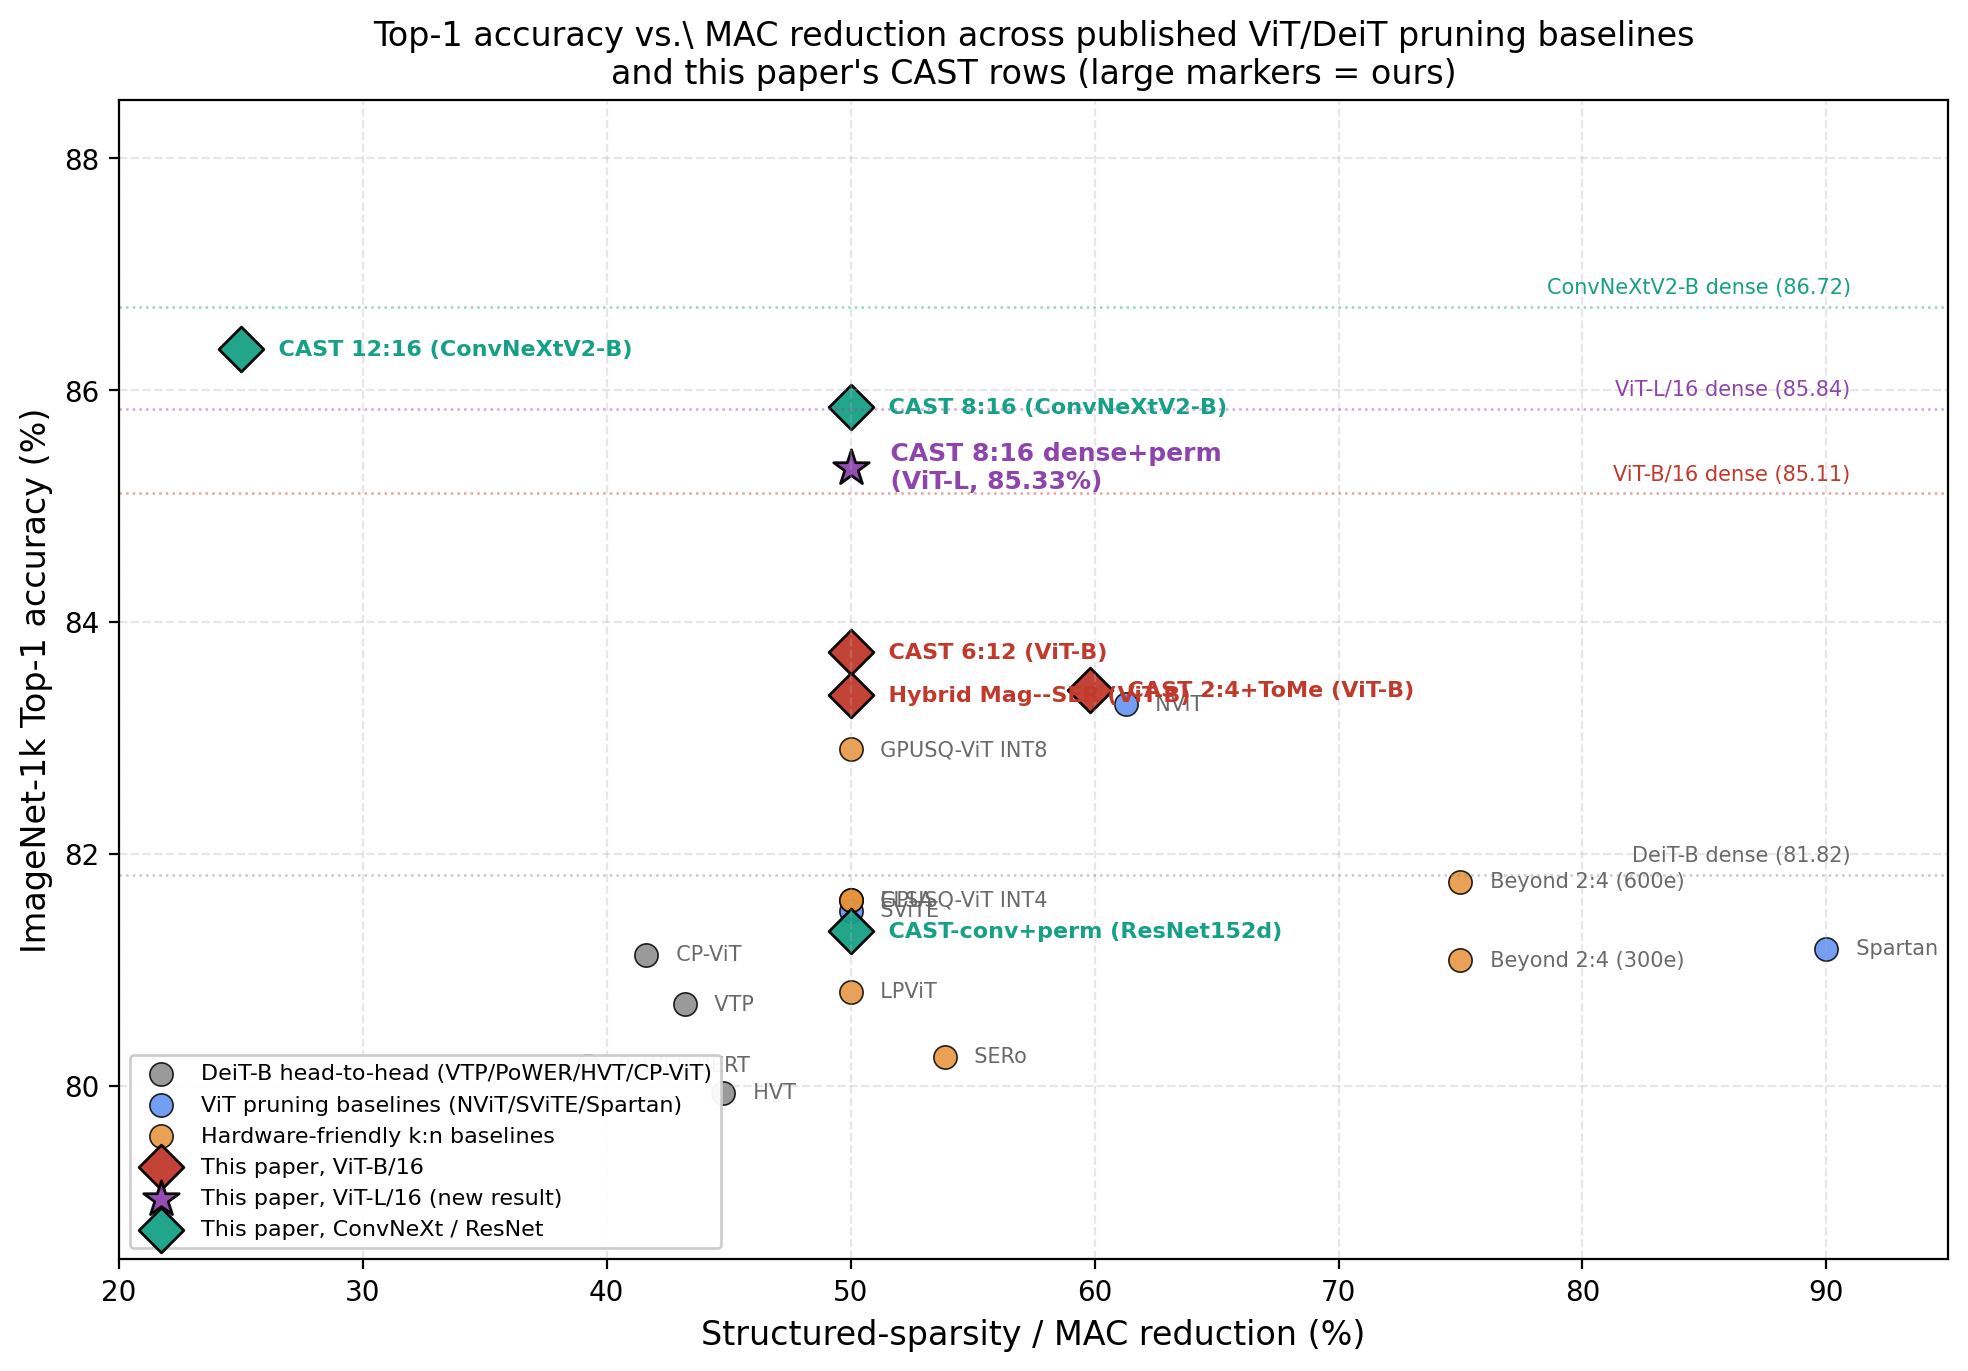
\includegraphics[width=0.95\linewidth]{comparison_top1_vs_macred.png}
\caption{Post-FT top-1 vs.\ reported sparse-execution MAC reduction. Points are rows from Table~\ref{tab:result_comparison}; marker size distinguishes this paper's CAST rows, color encodes architecture family, and dotted lines mark dense \texttt{timm} baselines. MAC reduction is computed against each cited method's own dense baseline.}
\label{fig:comparison_top1_vs_macred}
\end{figure}

\paragraph{CP-ViT \cite{song2022cp} DeiT context.}
CP-ViT reports DeiT-B results under a 30-epoch ImageNet fine-tuning protocol and reproduces VTP, PoWER-BERT, and HVT. Its Table~4 gives \(81.13\%\) post-FT top-1 at \(41.62\%\) FLOP reduction relative to an \(81.82\%\) dense DeiT-B baseline, a \(-0.69\) pp gap. Those rows evaluate token/cascade pruning rather than \(k{:}n\) weight sparsity, so they are included as DeiT-family context rather than as a matched weight-sparsity benchmark. In Figure~\ref{fig:comparison_top1_vs_macred}, CP-ViT appears at \((\sim 42\%,81.13\%)\); CAST \(8{:}16\) dense+perm on ViT-L/16 and CAST \(6{:}12\) on ViT-B/16 should be read as same-dataset but different-architecture/compression-axis points, with gaps reported against their own dense checkpoints.



Two observations follow from the table. Within this paper's ViT-B/16 unstructured \(50\%\) protocol, Hybrid Magnitude--SER is \(-1.7\) pp from dense, while the author-run SparseGPT-, Wanda-, and AlphaPruning-style rows are \(-4.0\), \(-3.8\), and \(-2.2\) pp under the same protocol. Across published rows, method ordering should be read with the protocol caveats below: Spartan, SViTE, and NViT use different sparsity definitions, training budgets, or architectures. The deployable CAST \(2{:}4{+}\)ToMe row has a \(-1.7\) pp accuracy gap and a measured \(1.41\times\) L4 speedup over the ToMe dense-kernel endpoint; the non-native \(6{:}12\) row reaches \(83.74\%\) at \(50\%\) structured sparsity as an accuracy result.

\paragraph{Protocol caveats.}
The rows in Table~\ref{tab:result_comparison} are not protocol-equivalent. They differ in pruned modules, compression axis, fine-tuning budget, validation usage, and dense baseline. For this paper's rows, the prunable-layer list is fixed across the 17-architecture sweep; masks are constructed without ImageNet validation access; validation is used to report completed checkpoints and in the documented sweeps used to choose global protocol settings. Results are reported against the corresponding \texttt{timm} dense checkpoint. The companion methodology paper gives the row-by-row protocol map (\S\,S.36 and \S\,S.37).

\subsection{Comparison with prior pruning methods}
\label{subsec:prior_method_comparison}

Detailed row provenance and protocol notes for VTP, PoWER-BERT, HVT, CP-ViT, OViT, NViT, SViTE, Spartan, X-Pruner, MiniViT, and AlphaPruning are in the companion methodology paper. Table~\ref{tab:result_comparison} reports the subset used for main-paper context.

\subsection{Limitations and scope}
\label{subsec:limitations}

The following empirical and methodological caveats delimit the claims of this paper.

\paragraph{Deployability of wider $k{:}n$ patterns.}
Only rows using a \(2{:}4\) mask are hardware-speedup claims under the tested PyTorch/NVIDIA sparse path. The \(6{:}12\), \(8{:}16\), and \(12{:}16\) rows impose structured sparsity and reduce arithmetic MAC counts in the model accounting, but they do not map to the native \(2{:}4\) Sparse Tensor Core path used for the measured speedups. They are therefore accuracy and MAC-accounting rows, not sparse-kernel throughput claims. The measured deployable row is ViT-B/16 \(2{:}4{+}\)ToMe at \(83.41\%\), with the A100 and L4 throughput measurements reported in Table~\ref{tab:param_to_flop_followup}.

\paragraph{ResNet152d $8{:}16$ projection at scale.}
No ResNet152d \(8{:}16\) dense+perm entry is reported. With \(n=16\), the certificate-projection step enumerates \(\binom{16}{8}=12{,}870\) candidate patterns per group and stores per-group covariance statistics; with the ResNet152d activation maps and default calibration batch, this exceeded a single 80\,GB A100 memory budget during certificate evaluation. The available ResNet152d entry is the CAST-conv+perm row at \(81.33\%\). Reporting an \(8{:}16\) ResNet152d counterpart would require streamed covariance evaluation or sharding of the certificate step.

\paragraph{ViT-L/16 \(85.33\%\) artifact status.}
The ViT-L/16 \(8{:}16\) dense+perm row is supported by the released \texttt{final\_eval.json}, recipe, logs, projected pre-FT checkpoint, and epoch-1/epoch-2 checkpoints. The final post-FT weights for the reported \(85.33\%\) row are not in the public bundle. Exact checkpoint-level reproduction therefore requires resuming the released recipe from the epoch-2 artifact for the remaining epoch; the released JSON records the reported evaluation result.

\paragraph{Data and checkpoint availability.}
Code is available at \url{https://github.com/yspennstate/RMT_based_pruning_in_deep_learning}. The public artifact bundle is the Google Drive folder listed in the README and indexed by \texttt{data/release\_manifest.json}. The manifest records zip names, sizes, row-to-evidence paths, and checkpoint availability. The release includes the 17-model Hybrid Magnitude--SER checkpoint archive, SER \(s=0.35\) source checkpoints, available CAST/FLOP-model checkpoints, \texttt{final\_eval.json} logs for bundled CAST rows, the 282-cell certificate audit, mask-statistics files, and run logs. ImageNet-1k images are not redistributed; reproduction scripts expect the user to provide ImageNet-1k train/validation data. Rows supported by logs/evaluation JSON and recipe rather than a final post-FT checkpoint are explicitly marked in the manifest.

\paragraph{Analytic Lipschitz constants.}
The deterministic data-path budget
\[
B_T(R) = (2/|T|)\sum_s L_s\|R\psi_1(s)\|_\infty
\]
contains per-sample post-layer Lipschitz constants \(L_s\). The theorems condition on such constants, but this paper does not compute certified \(L_s\) values for transformer blocks. The empirical audit therefore uses \(\hat B_T=\|R\|_{\mathrm{op}}\cdot\overline{\|\psi\|_\infty}\) as a diagnostic predictor of realized top-1 drop, not as an upper bound on \(B_T(R)\). Tight certified bounds for modern transformer blocks remain future work.

\paragraph{Generalized statements: proof scope.}
Section~\ref{sec:abstract_additive_extensions} generalizes the Gaussian instance of Appendix~\ref{Main_theory} by replacing Gaussian Assumptions~\ref{as2}--\ref{as3} with Assumptions~\ref{as4}--\ref{as6} and Lemma~\ref{lem:remove_R} with Lemma~\ref{lem:remove_R_general}. The proofs used for the empirical certificate interpretation are collected in Appendices~\ref{app:proof_perturb}--\ref{app:proofs_main}.

\paragraph{Seed variance.}
Most CAST rows in Tables~\ref{tab:param_to_flop_followup} and~\ref{tab:result_comparison} are single-seed runs under a fixed recipe. In ablations with repeated seeds, such as the ViT-B/16 cert-source sweep, the across-seed standard deviation of post-FT top-1 was within \(\pm0.15\) pp. Comparable repeats were not run for the ViT-L/16, ConvNeXtV2-B, and ResNet \(8{:}16\) result rows, so the \(85.33\%\) and \(86.35\%\) entries, and the ViT-L/16 \(-0.51\) pp dense gap, should be read as point estimates rather than confidence intervals.

\paragraph{Methodological provenance.}
The main manuscript gives the theoretical statements, proof references, algorithm summaries, and headline numerical tables. The companion methodology paper records the operational provenance for several choices: the SER hyperparameter sweep selecting \(s=0.35\) for the CAST \(2{:}4{+}\)ToMe source; BEMA fitting of the per-layer MP edge \(\sigma_+(\ell)\); the full 282-cell certificate audit; and the row-level extraction protocols for the prior-method comparison. These companion sections are the audit trail for hyperparameters, edge fitting, certificate-audit construction, and literature-row provenance.

\paragraph{Future work.}
Three extensions follow from the present framework: (a) a streaming or multi-GPU cert-projection implementation that lifts the ResNet152d \(8{:}16\) barrier and enables routine \(k{:}n\) projection on \(>100\)M-parameter ConvNets; (b) explicit numerical estimation of \(L_s\) for representative transformer blocks, replacing the operator-norm proxy in the budget \(B_T(R)\) with a certified upper bound; (c) extending CAST to sparse tensor-core kernels beyond the native \(2{:}4\) pattern. If future hardware or software exposes native kernels for wider patterns, the corresponding throughput would need to be measured separately; in this paper the \(6{:}12\), \(8{:}16\), and \(12{:}16\) rows are accuracy and MAC-accounting studies.

\FloatBarrier
\section{Abstract Additive Perturbation Extensions}
\label{sec:abstract_additive_extensions}

This section gives the additive \(W=S+R\) version of the deterministic certificate analysis. It complements the mask certificates of Section~\ref{Main_theory_gen}; the Gaussian specialization and spectral consequences appear in Appendix~\ref{Main_theory}.

The results below generalize the Gaussian logit-perturbation, loss-reduction, pathwise denoising, stationarity-collapse, and BBP-type statements of Appendix~\ref{Main_theory}.

\subsection{Assumptions for the generalized perturbation framework}
\label{gen_ass_for_R}

Throughout the asymptotic statements in this section, the training set \(T\) is finite and fixed independently of \(N\), unless a result explicitly states summability conditions for a growing family.

\begin{assumption}[General architecture]
\label{as4}
Assume the DNN can be written as
\[
\phi=\rho\circ \psi_2\circ (R+S)\circ \psi_1,
\]
where \(\psi_1,\psi_2\) may depend on the remaining network parameters and \(\rho\) is softmax. For each \(s\in T\), let \(\mathcal U_s\) be any set containing the admissible interpolation segment \(\{(S+\vartheta R)\psi_1(s):\vartheta\in[0,1]\}\). We assume that \(\psi_2\) has a finite local Lipschitz constant with respect to \(\ell_\infty\) on \(\mathcal U_s\):
\[
L_{\psi_2}(s)
:=
\sup_{v\neq w}
\frac{\|\psi_2(v)-\psi_2(w)\|_{\infty}}{\|v-w\|_{\infty}}
<\infty.
\]
Here the supremum is taken only over \(\mathcal U_s\), so only a local-on-the-path Lipschitz bound is required.
\end{assumption}

\begin{rem}[Interpretation of Assumption~\ref{as4}]
This assumption fixes notation.  After freezing all other weights, the network is factored around the layer being studied: \(\psi_1(s)\) is the input activation to that layer, \(R+S\) is the layer matrix, and \(\psi_2\) maps the layer output to logits.  The Lipschitz constant is required only on the finite path traced by the interpolation \(S+\vartheta R\), not globally on the whole ambient space.  For ReLU or piecewise-linear networks this is automatic on bounded paths; for architectures with normalization layers it is an explicit local regularity condition, excluding only pathological paths where the post-layer map becomes singular.  In the Gaussian model of Appendix~\ref{Main_theory}, Assumption~\ref{as1} is the concrete three-layer instance of this factorization with the target layer \(W_2=S_2+R_2\).
\end{rem}

\begin{assumption}[Perturbative random component]
\label{as5}
Assume that for every deterministic vector \(v\), and more generally for every \(v\) measurable with respect to the conditioning variables \(\sigma(S,\psi_1,\psi_2)\),
\begin{equation}
\label{eq:general_perturb_assumption}
\PP\Big(\|Rv\|_{\infty}>d_1(N)J(v)\,\Big|\,S,\psi_1,\psi_2\Big)\le d_2(N),
\end{equation}
where \(d_1(N),d_2(N)\to0\) and \(J(v)\) depends only on \(v\). When a spectral interpretation is desired, we additionally assume that the singular-value ESD of \(R\) converges to a deterministic law with finite right edge \(b_+<\infty\).
\end{assumption}

\begin{rem}[Interpretation of Assumption~\ref{as5}]
The vector \(v\) is fixed before the randomness in \(R\) is revealed.  In the network application \(v=\psi_1(s)\), so the pre-layer activation is treated as part of the conditioning information.  The assumption does not require Gaussian entries; it requires only that every data activation is sent by \(R\) to a small vector in \(\ell_\infty\) norm, with high probability.  The optional empirical-spectral-distribution condition is used only for RMT interpretation and spectral corollaries.  The loss and certificate bounds use the concentration estimate \eqref{eq:general_perturb_assumption}, not the ESD convergence.

The Gaussian connection is explicit: Assumption~\ref{as2} in Appendix~\ref{Main_theory} implies Assumption~\ref{as5} with \(J(v)=\|v\|_2\) and \(d_1(N)\) of order \(\sqrt{\log N/N}\).  The confidence-parameter version is Theorem~\ref{thm:finite_confidence_gaussian}; the MP-edge interpretation of the same variance scale is Corollary~\ref{cor:mp_edge_data_path_budget}.
\end{rem}

\begin{ex}
If \(R\) has i.i.d.\ Gaussian entries with variance \(1/N\), then
\[
\PP\!\left(
\|Rv\|_\infty
>
2\sqrt{2}\,\|v\|_2\sqrt{\frac{\log(2N)}{N}}
\right)
\le
\frac{1}{N},
\]
so Assumption~\ref{as5} holds with \(d_1(N)=2\sqrt{2\log(2N)/N}\), \(d_2(N)=1/N\), and \(J(v)=\|v\|_2\). The concrete three-layer Gaussian specialization is Lemma~\ref{lem:remove_R} and Theorem~\ref{thm:finite_confidence_gaussian} in Appendix~\ref{Main_theory}; the proof of the abstract concentration step is in Appendix~\ref{app:proof_perturb}. The same conditional formulation also accommodates sub-Gaussian rows, orthogonally invariant perturbations, or moderate training-induced dependence, provided the displayed concentration estimate survives.
\end{ex}

\begin{ex}[Sub-Gaussian rows]
\label{ex:subgaussian_rows}
Assume, conditionally on \(S,\psi_1,\psi_2\), that the rows \(r_1,\dots,r_N\) of \(R\) are independent, centered, and satisfy
\[
\|\langle r_j,v\rangle\|_{\psi_2}
\le
\frac{\kappa}{\sqrt N}\|v\|_2
\qquad
\text{for all }v\text{ and all }j.
\]
Then there is a universal constant \(C\) such that, for every \(\delta\in(0,1)\),
\[
\PP\!\left(
\|Rv\|_\infty
>
C\kappa\|v\|_2\sqrt{\frac{\log(2N/\delta)}{N}}
\,\middle|\,S,\psi_1,\psi_2
\right)
\le \delta.
\]
Thus this sufficient condition is not intrinsically Gaussian; it uses row-wise concentration at the \(N^{-1/2}\sqrt{\log N}\) scale.
\end{ex}

\begin{assumption}[Structured component for optional spectral conclusions]
\label{as6}
Whenever a spectral conclusion is invoked, assume that there exists a sequence \(k_N=o(\min\{N,M\})\) such that
\[
\sum_{i>k_N}s_i(S)^2\to0.
\]
The convergence is in probability when \(S\) is random.
\end{assumption}

\begin{rem}[Interpretation of Assumption~\ref{as6}]
This assumption is used only when the paper draws spectral conclusions about the structured part \(S\).  It is not needed for the loss-reduction theorems, the data-path certificate, or the stationarity-collapse inequality.  The condition means that all but \(o(\min\{N,M\})\) singular directions of \(S\) carry vanishing squared singular-value mass.

Exact finite rank is the simplest case.  If \(\rank(S)\le r_0\) for a constant \(r_0\), take \(k_N=r_0\).  Then \(k_N=o(\min\{N,M\})\) and \(\sum_{i>k_N}s_i(S)^2=0\), so Assumption~\ref{as6} holds automatically.  More generally, if \(\rank(S)=r_N=o(\min\{N,M\})\), take \(k_N=r_N\).  Approximate low rank allows a small tail: the rank may not be exactly finite, but the singular-value energy beyond \(k_N\) must vanish.  The Gaussian analogue is Assumption~\ref{as3spectral} in Appendix~\ref{Main_theory}.
\end{rem}

For a DNN satisfying Assumption~\ref{as4}, define
\begin{equation}
\label{from_DNN_st_2}
h_\phi(s):=J(\psi_1(s))\,L_{\psi_2}(s).
\end{equation}

The remaining hypotheses appearing in the theorems are quantitative smallness conditions rather than structural assumptions.  The condition \(a_\phi(N,s)=h_\phi(s)d_1(N)\to0\) requires the random-like component to be weak after propagation through the data path.  The condition \(\langle S,R\rangle_F=o_{\PP}(1)\) requires the regularizer to have no persistent first-order cross term when \(R\) is removed.  In the Gaussian appendix, Assumption~\ref{as1} supplies the corresponding data-path scaling and Assumption~\ref{as3} supplies the cross-term control.  Finally, the one-sided stationarity hypotheses in Theorems~\ref{main_result_reducing_noise_general} and~\ref{main_result_reducing_noise} are not random-matrix assumptions; they require the trained model to be nearly stationary in the particular denoising direction being tested.

\subsection{Generalized perturbation and loss-reduction results}
\label{decrease_in_loss}

We consider the regularized loss
\begin{equation}
\label{loss_noise_det_2}
L(\alpha(t))
=
-\frac{1}{|T|}\sum_{s\in T}\log\big(\phi_{C(s)}(s,\alpha(t))\big)
+
\lambda_{\mathrm{reg}}
\sum_{i=1}^{L}\|W_i(t)\|_F^2.
\end{equation}

\begin{lem}
\label{lem:remove_R_general}
Let
\[
X=\psi_2\circ (R+S)\circ \psi_1(s),
\]
and let \(\alpha_W,\alpha_S\) denote the corresponding network parameters when the relevant weight matrix is \(W=R+S\) and \(S\), respectively. Under Assumptions~\ref{as4}--\ref{as5},
\[
\PP\Big(
\|X(s,\alpha_S)-X(s,\alpha_W)\|_\infty
\le d_1(N)h_\phi(s)
\Big)
\ge 1-d_2(N).
\]
\end{lem}
\proofloc{See Appendix~\ref{app:proof_perturb}, Proof of Lemma~\ref{lem:remove_R_general}.}

\begin{thm}
\label{theorem_reduction_of_loss_general}
Assume Assumptions~\ref{as4}--\ref{as5} and that
\[
\langle S,R\rangle_F\to0
\qquad\text{in probability as }N\to\infty.
\]
Assume further that for all \(s\in T\),
\[
a_\phi(N,s):=h_\phi(s)d_1(N)\to0
\qquad\text{as }N\to\infty.
\]
Then removing \(R\) yields
\[
L(\alpha_S)=L(\alpha_W)-\lambda_{\mathrm{reg}}\|R\|_F^2+o_{\PP}(1)
\qquad(N\to\infty).
\]
\end{thm}
\proofloc{See Appendix~\ref{app:proofs_abstract_generalizations}, Proof of Theorem~\ref{theorem_reduction_of_loss_general}.}

In the square three-layer Gaussian model, Theorem~\ref{theorem_reduction_of_loss} in Appendix~\ref{Main_theory} gives the corresponding finite-\(N\) loss-reduction statement, and Theorem~\ref{thm:finite_confidence_gaussian} gives the confidence-parameter version.

\begin{cor}[Growing-set abstract loss reduction]
\label{cor:growing_set_abstract_loss}
Let \(T_N\) be a finite labeled set that may depend on \(N\). Let \(L_{\cancel{\mathrm{reg}},T_N}\) denote cross-entropy averaged over \(T_N\), and let \(L_{T_N}\) denote the corresponding regularized objective with the same Frobenius penalty as in \eqref{loss_noise_det_2}. Assume Assumptions~\ref{as4}--\ref{as5},
\[
\langle S,R\rangle_F=o_{\PP}(1),
\qquad
|T_N|d_2(N)\to0,
\]
and
\[
\frac{1}{|T_N|}\sum_{s\in T_N}a_\phi(N,s)\to0
\]
in probability. Then
\[
L_{T_N}(\alpha_S)
=
L_{T_N}(\alpha_W)
-\lambda_{\mathrm{reg}}\|R\|_F^2
+o_{\PP}(1).
\]
\end{cor}
\proofloc{See Appendix~\ref{app:proofs_abstract_generalizations}, Proof of Corollary~\ref{cor:growing_set_abstract_loss}.}

\begin{cor}
\label{cor:scaled_reduction_of_loss_general}
Under the hypotheses of Theorem~\ref{theorem_reduction_of_loss_general}, for any fixed \(\vartheta\in[0,1]\), define
\[
W(\vartheta)=S+\vartheta R.
\]
Then
\[
L(\alpha_{W(\vartheta)})
=
L(\alpha_W)-\lambda_{\mathrm{reg}}(1-\vartheta^2)\|R\|_F^2+o_{\PP}(1)
\qquad(N\to\infty).
\]
The same asymptotic statement holds along any deterministic sequence \(\vartheta_N\in[0,1]\).
\end{cor}
\proofloc{See Appendix~\ref{app:proofs_abstract_generalizations}, Proof of Corollary~\ref{cor:scaled_reduction_of_loss_general}.}

\begin{cor}[Finite-\(N\) scaled loss bound along the denoising path]
\label{cor:scaled_reduction_of_loss_general_finiteN}
Assume the hypotheses of Theorem~\ref{theorem_reduction_of_loss_general}, and define \(W(\vartheta)=S+\vartheta R\) for \(\vartheta\in[0,1]\). Then for every \(\eta>0\) there exists an event \(E_{N,\eta}\) with
\[
\PP(E_{N,\eta})\ge 1-|T|d_2(N)-\PP\!\big(|\langle S,R\rangle_F|>\eta\big)
\]
such that on \(E_{N,\eta}\),
\[
L(\alpha_{W(\vartheta)})
\le
L(\alpha_W)
-\lambda_{\mathrm{reg}}(1-\vartheta^2)\|R\|_F^2
+(1-\vartheta)\frac{2}{|T|}\sum_{s\in T}a_\phi(N,s)
+2\lambda_{\mathrm{reg}}(1-\vartheta)\eta
\]
for every \(\vartheta\in[0,1]\).
\end{cor}
\proofloc{See Appendix~\ref{app:proofs_abstract_generalizations}, Proof of Corollary~\ref{cor:scaled_reduction_of_loss_general_finiteN}.}

The Gaussian pathwise analogue is Corollary~\ref{cor:scaled_reduction_of_loss} in Appendix~\ref{Main_theory}; it is the specialization used in the Gaussian stationarity-collapse theorem.

\begin{thm}[Multi-layer telescoping loss reduction]
\label{thm:multilayer_telescoping}
Let \(\mathcal P\) be a finite set of layers selected for pruning, with \(|\mathcal P|\) fixed independently of \(N\). For each \(\ell\in\mathcal P\), write
\[
W_\ell=S_\ell+R_\ell,
\]
and assume that, after the previous layers in \(\mathcal P\) have already been replaced by their structured parts, the single-layer hypotheses of Theorem~\ref{theorem_reduction_of_loss_general} continue to hold for layer \(\ell\) with perturbation scale \(a_{\phi,\ell}(N,s)\). If \(\alpha^{(0)}\) denotes the original network parameters and \(\alpha^{(|\mathcal P|)}\) the parameters after replacing every \(W_\ell\) by \(S_\ell\), then
\[
L(\alpha^{(|\mathcal P|)})
=
L(\alpha^{(0)})
-\lambda_{\mathrm{reg}}\sum_{\ell\in\mathcal P}\|R_\ell\|_F^2
+o_{\PP}(1).
\]
Thus the one-layer denoising theorem extends to the stylized multi-layer pruning pipeline by telescoping the loss differences over the pruned layers.

More generally, the set of pruned layers may depend on \(N\). Let \(\mathcal P_N\) be a sequence of layer sets, ordered in the pruning order. Assume that the corresponding one-layer logit events \(E_{\ell,N}\) satisfy
\[
\sum_{\ell\in\mathcal P_N}\PP(E_{\ell,N}^c)\to0,
\]
that their perturbation scales are summable,
\[
\sum_{\ell\in\mathcal P_N}\frac{1}{|T|}\sum_{s\in T}a_{\phi,\ell}(N,s)\to0,
\]
and that the accumulated cross term is negligible,
\[
\sum_{\ell\in\mathcal P_N}\langle S_\ell,R_\ell\rangle_F=o_{\PP}(1).
\]
Then the same telescoping conclusion holds with \(\mathcal P\) replaced by \(\mathcal P_N\).
\end{thm}
\proofloc{See Appendix~\ref{app:proofs_abstract_generalizations}, Proof of Theorem~\ref{thm:multilayer_telescoping}.}

\begin{rem}[Beyond pure Frobenius regularization]
\label{rem:bregman_regularizer}
The quadratic penalty in \eqref{loss_noise_det_2} is used only to obtain a coercive lower bound of order \(\|R\|_F^2\). For a general differentiable \(\mu\)-strongly convex regularizer \(\Omega\), one has the exact decomposition
\[
\Omega(S+R)-\Omega(S)
=
\langle \nabla\Omega(S),R\rangle + D_\Omega(S+R,S),
\]
where
\[
D_\Omega(S+R,S)\ge \frac{\mu}{2}\|R\|_F^2.
\]
Thus the same extension is valid provided the first-order term \(\langle \nabla\Omega(S),R\rangle\) is controlled or negligible along the admissible sequence. In the Frobenius case \(\Omega(W)=\|W\|_F^2\), this term is exactly \(2\langle S,R\rangle_F\), which is already part of the hypotheses. For the elastic-net penalty
\[
\Omega(W)=\mu_1\|W\|_1+\mu_2\|W\|_F^2,
\qquad \mu_2>0,
\]
the \(L_1\) term is nonsmooth and can increase when \(R\) is removed if \(R\) cancels entries of \(S\). The correct extension is subgradient-based: choose \(\xi\in\partial\|S\|_1\) and assume
\[
\langle \mu_1\xi+2\mu_2S,R\rangle=o_{\PP}(1).
\]
The quadratic part then supplies the strong convexity needed for the same type of loss-reduction bound.
\end{rem}

\begin{thm}
\label{main_result_reducing_noise_general}
Assume Assumptions~\ref{as4}--\ref{as5}. Assume further that for all \(s\in T\),
\[
a_\phi(N,s):=h_\phi(s)d_1(N)\to0
\qquad\text{as }N\to\infty.
\]
Suppose:
\begin{enumerate}[leftmargin=2em]
\item for each \(N\), \(\alpha(t,N)\to \alpha^*(N)\) in probability as \(t\to\infty\);
\item the relevant limit weight matrix admits an admissible decomposition \(W^*(N)=S^*(N)+R^*(N)\) satisfying
\[
\langle S^*(N),R^*(N)\rangle_F\to0
\qquad\text{in probability as }N\to\infty.
\]
\end{enumerate}
\noindent For \(\vartheta\in[0,1]\), let \(\alpha_\vartheta^*(N)\) denote the parameter vector obtained by replacing \(W^*(N)\) with \(S^*(N)+\vartheta R^*(N)\). Assume further that there exists a sequence of nonnegative random variables \(\epsilon_N=o_{\PP}(1)\) such that the one-sided directional stationarity event
\[
\liminf_{h\downarrow0}
\frac{
L(\alpha_{1-h}^*(N))-L(\alpha^*(N))
}{h}
\ge -\epsilon_N
\]
has probability tending to one.
Define
\[
\bar a_{\phi,N}:=\frac{2}{|T|}\sum_{s\in T}a_\phi(N,s).
\]
Then
\[
\|R^*(N)\|_F^2
\le
\frac{\bar a_{\phi,N}+\epsilon_N}{2\lambda_{\mathrm{reg}}}
+o_{\PP}(1).
\]
In particular, if \(\bar a_{\phi,N}+\epsilon_N\to0\) in probability, then for every \(\epsilon>0\),
\[
\lim_{N\to\infty}\PP\big(\|R^*(N)\|_F\le \epsilon\big)=1.
\]

If, in addition, there exists an admissible path decomposition
\[
W(t,N)=S(t,N)+R(t,N)
\]
such that for each fixed \(N\),
\[
\|S(t,N)-S^*(N)\|_F+\|R(t,N)-R^*(N)\|_F\to0
\qquad\text{in probability as }t\to\infty,
\]
and if for every fixed \(N\) and every \(\epsilon>0\),
\[
\PP\big(\|R^*(N)\|_F=\epsilon\big)=0,
\]
then
\[
\lim_{N\to\infty}\lim_{t\to\infty}\PP\big(\|R(t,N)\|_F\le \epsilon\big)=1.
\]
\end{thm}
\proofloc{See Appendix~\ref{app:proofs_abstract_generalizations}, Proof of Theorem~\ref{main_result_reducing_noise_general}.}

Appendix~\ref{Main_theory} gives the concrete Gaussian/RMT version of this conclusion: Theorem~\ref{main_result_reducing_noise} proves collapse of the admissible Gaussian component, Corollary~\ref{cor:variance_scale_collapse} translates this into collapse of the MP variance scale, and Corollary~\ref{cor:bulk_collapse_spike_stabilization} records the resulting spectral stabilization.

\begin{rem}
The theorem assumes only one-sided directional approximate stationarity at the unpruned point \(\vartheta=1\). Exact local minimality is a sufficient special case with \(\epsilon_N\equiv0\), but the hypothesis is weaker than a global lower bound along the whole denoising path. Without the continuity assumption \(\PP(\|R^*(N)\|_F=\epsilon)=0\), the same proof still gives the weaker limsup/liminf bounds obtained from Portmanteau-type arguments, but not necessarily exact convergence of the probabilities at the threshold \(\epsilon\).
\end{rem}

\begin{cor}[Eventual supercriticality of persistent spike clusters in a BGN-type deformation regime]
\label{cor:general_BGN_persistent_spikes}
Under the hypotheses of Theorem~\ref{main_result_reducing_noise_general}, assume additionally that for each \(N\) the pair \(W^*(N)=S^*(N)+R^*(N)\) lies in a finite-rank deformation regime satisfying all hypotheses of Theorem~\ref{thm:abstract_inverse_D} for the spikes considered below. In particular, assume the regime has a deterministic bulk edge \(b_+(N)\), a deterministic critical threshold \(\theta_c(N)\), a strictly decreasing outlier transform
\[
D_N:(b_+(N),\infty)\to (0,D_N(b_+(N)^+))
\]
in the sense of Appendix~\ref{app:proofs_main}, local Lipschitz/invertibility intervals around the outliers, and concentration of the relevant sample singular values in those intervals. Assume that
\[
\theta_c(N)\to0,
\qquad
b_+(N)\to0.
\]
Assume further that for some fixed \(k\ge1\) there exist constants
\[
\bar\sigma_1>\cdots>\bar\sigma_k>0
\]
such that
\[
\sigma_i^*(N)\to\bar\sigma_i
\qquad\text{in probability as }N\to\infty
\]
for each \(1\le i\le k\). Then:
\begin{enumerate}[leftmargin=2em]
\item
\[
\PP\!\big(\sigma_i^*(N)>\theta_c(N)\big)\to1
\qquad\text{for each }1\le i\le k;
\]
\item these \(k\) spikes are eventually supercritical, so the corresponding singular values of \(W^*(N)\) form outlier clusters above the edge \(b_+(N)\). Moreover, if the \(i\)-th spike is separated from the other nonzero singular values of \(S^*(N)\) by a gap \(\Delta_i(N)>0\) with
\[
\frac{\|R^*(N)\|_{\op}}{\Delta_i(N)}\to0
\qquad\text{in probability},
\]
then the associated rank-one left and right spectral projectors converge in operator norm to the corresponding projectors of \(S^*(N)\);
\item defining the inverse-\(D\) estimator on the event \(s_i(W^*(N))>b_+(N)\), whose probability tends to one, by
\[
\widehat\sigma_i^{(D)}(N):=D_N(s_i(W^*(N)))^{-1/2},
\]
and defining it arbitrarily off that event,
one has
\[
\widehat\sigma_i^{(D)}(N)-\sigma_i^*(N)\to0
\qquad\text{in probability}
\]
for each \(1\le i\le k\).
\end{enumerate}
\end{cor}
\proofloc{See Appendix~\ref{app:proofs_abstract_generalizations}, Proof of Corollary~\ref{cor:general_BGN_persistent_spikes}.}

For the square Gaussian finite-rank case, the corresponding RMT statement is Corollary~\ref{cor:gaussian_BBP_persistent_spikes} in Appendix~\ref{Main_theory}; the external BGN input and the inverse-\(D\) abstraction are stated in Appendix~\ref{app:proofs_main}.

\begin{rem}
Corollary~\ref{cor:general_BGN_persistent_spikes} is the abstract analogue of the Gaussian BBP statement. It says that once a finite-rank deformation model has a well-defined critical threshold \(\theta_c(N)\), vanishing admissible randomness forces every structurally persistent spike cluster to cross that threshold eventually. Thus the limit theory does not merely predict collapse of the random bulk; it predicts a detectability transition for persistent informative directions in any deformation regime governed by an inverse-\(D\) outlier map.
\end{rem}

\begin{rem}[Assumption map for the abstract and deterministic theory]
The following list summarizes which assumptions are used by the abstract additive results in this section and by the deterministic mask results in Section~\ref{Main_theory_gen}:
\begin{enumerate}[leftmargin=2em]
\item Lemma~\ref{lem:deterministic_ce_path_bound}, Corollaries~\ref{cor:deterministic_margin_stability}, \ref{cor:restoration_improves_certificate}, \ref{cor:weighted_mask_certificate}, \ref{cor:weighted_mask_stationarity}, and \ref{cor:deterministic_multilayer_margin_stability}, and Theorems~\ref{thm:deterministic_additive_frobenius_certificate}--\ref{thm:deterministic_multilayer_mask_stationarity} are deterministic statements. They do not assume an additive Gaussian decomposition; the mask-specific results use only disjoint support of the kept, restored, and removed entries.
\item Corollaries~\ref{cor:gaussian_data_path_budget}--\ref{cor:multilayer_subgaussian_data_path_budget} give random sufficient conditions for the deterministic data-path budgets.
\item Lemma~\ref{lem:remove_R_general} uses only Assumptions~\ref{as4}--\ref{as5}.
\item Theorem~\ref{theorem_reduction_of_loss_general}, Corollary~\ref{cor:scaled_reduction_of_loss_general}, and the finite-\(N\) pathwise Corollary~\ref{cor:scaled_reduction_of_loss_general_finiteN} use Assumptions~\ref{as4}--\ref{as5} together with the additional hypotheses \(\langle S,R\rangle_F=o_{\PP}(1)\) and \(a_\phi(N,s)\to0\) for each \(s\in T\). Assumption~\ref{as6} is not needed for these loss bounds. Their concrete Gaussian counterparts are Theorem~\ref{theorem_reduction_of_loss} and Corollary~\ref{cor:scaled_reduction_of_loss} in Appendix~\ref{Main_theory}.
\item Theorem~\ref{thm:multilayer_telescoping} is obtained by applying Theorem~\ref{theorem_reduction_of_loss_general} layer by layer; the second part allows a growing layer set under summable perturbation and failure-probability conditions.
\item Theorem~\ref{main_result_reducing_noise_general} uses Assumptions~\ref{as4}--\ref{as5}, the same scaling condition \(a_\phi(N,s)\to0\), the cross-term condition at the limit point, and the one-sided directional stationarity hypothesis stated in the theorem. Its Gaussian counterpart is Theorem~\ref{main_result_reducing_noise}, with MP variance and spectral consequences in Corollaries~\ref{cor:variance_scale_collapse}--\ref{cor:bulk_collapse_spike_stabilization}.
\item Corollary~\ref{cor:general_BGN_persistent_spikes} further assumes that the pair \(W^*(N)=S^*(N)+R^*(N)\) satisfies the finite-rank deformation hypotheses of Theorem~\ref{thm:abstract_inverse_D}, a threshold \(\theta_c(N)\to0\), an edge \(b_+(N)\to0\), and a persistent-spike hypothesis \(\sigma_i^*(N)\to\bar\sigma_i>0\). The square Gaussian BBP specialization is Corollary~\ref{cor:gaussian_BBP_persistent_spikes}.
\item The pathwise conclusion in Theorem~\ref{main_result_reducing_noise_general} additionally uses the path-decomposition convergence assumption, while the no-atom condition \(\PP(\|R^*(N)\|_F=\epsilon)=0\) is only needed for exact convergence of the probabilities at the threshold \(\epsilon\).
\end{enumerate}
\end{rem}




% =================================================
\FloatBarrier
\section{Main Theoretical Results: Deterministic Pruning Certificates}
\label{Main_theory_gen}
% =================================================

This section contains the main theory used to interpret the pruning experiments.  The central deterministic object is the propagated effect of the removed component on the logits.  Random-matrix assumptions enter only as sufficient conditions for this deterministic certificate, rather than as an assumption that a trained ViT layer is literally a low-rank matrix plus independent Gaussian noise.

The proof chain is organized as follows.  Lemma~\ref{lem:deterministic_ce_path_bound} turns a data-path perturbation bound into a cross-entropy perturbation bound, and Corollary~\ref{cor:deterministic_margin_stability} gives the corresponding margin-stability statement.  Theorem~\ref{thm:deterministic_mask_certificate} is the main certificate for actual unstructured masks, while Theorem~\ref{thm:deterministic_prune_restore_certificate} and Corollary~\ref{cor:restoration_improves_certificate} specialize it to prune--restore/SER-style masks.  Theorems~\ref{thm:deterministic_multilayer_mask_certificate} and~\ref{thm:deterministic_multilayer_mask_stationarity} give the finite multi-layer versions.  Corollaries~\ref{cor:gaussian_data_path_budget}--\ref{cor:multilayer_subgaussian_data_path_budget} then show that Gaussian or sub-Gaussian random components satisfy the required data-path budgets with high probability, and Corollary~\ref{cor:mp_edge_data_path_budget} rewrites the Gaussian budget directly in terms of the MP singular-value edge.

The abstract additive perturbation framework in Section~\ref{sec:abstract_additive_extensions} gives the complementary \(W=S+R\) viewpoint, while Appendix~\ref{Main_theory} contains the stylized Gaussian loss-reduction and spectral-collapse specialization.  Each theorem, lemma, and corollary in the main text includes a proof-location note pointing to the appendix proof.


\begin{rem}[Regularisation scaling]
\label{rem:lambda_reg_scaling}
Throughout the loss-reduction statements of Section~\ref{Main_theory_gen} and the Gaussian appendix (Appendix~\ref{Main_theory}), the elastic-net penalty coefficients $\lambda_1, \lambda_2$ are treated as fixed quantities. In particular, an iid-Gaussian admissible component $R \in \mathbb{R}^{N \times N}$ with entries of variance $g/N$ has $\|R\|_F^2 = \Theta(gN)$ in expectation, so the loss-reduction term $\lambda_2 \|R\|_F^2$ scales as $\Theta(\lambda_2 g N)$. The coefficient $\lambda_2$ may represent either (i) an absolute weight-decay coefficient applied uniformly across the network, or (ii) a normalised version rescaled by parameter count, depending on the deployment. The certificate inequality of Theorem~\ref{thm:deterministic_mask_certificate} holds for any specified $\lambda_1, \lambda_2$. If the regulariser is normalised by parameter count or layer width, the same theorem applies with the corresponding normalised coefficients, but the numerical certificate margin changes accordingly. The data-path budget $B_T(R)$ is independent of $\lambda_1, \lambda_2$, whereas the elastic-net reward $\lambda_2 \|R\|_F^2 + \lambda_1 \|R\|_1$ is not. The certificate condition therefore depends on the regulariser scale; the qualitative comparison between the data-path budget and the elastic-net budget is unchanged.
\end{rem}

\subsection{Deterministic data-path certificates for mask pruning}
\label{subsec:deterministic_mask_certificate}

Fix one target layer \(A\in\R^{n\times m}\) inside a network and write the logits as
\[
z_A(s):=\psi_2(A\psi_1(s))\in\R^K,
\qquad s\in T,
\]
where \(\psi_1\) and \(\psi_2\) denote the pre-layer and post-layer computations with all other parameters frozen. For a decomposition
\[
A=S+R,
\qquad
A_\theta:=S+\theta R,\qquad 0\le\theta\le1,
\]
let \(L_s\) be any finite deterministic upper bound on the local \(\ell_\infty\)-Lipschitz constant of \(\psi_2\) on the path
\[
\{A_\theta\psi_1(s):0\le\theta\le1\}.
\]
Define the data-path budget of the removed component by
\begin{equation}
\label{eq:data_path_budget}
B_T(R):=
\frac{2}{|T|}\sum_{s\in T}L_s\|R\psi_1(s)\|_\infty.
\end{equation}
If \(L_s\) is itself estimated from the realized network, the statements below are deterministic conditional on that realized upper bound.

\begin{lem}[Deterministic cross-entropy path bound]
\label{lem:deterministic_ce_path_bound}
For every decomposition \(A=S+R\) and every \(\theta\in[0,1]\),
\[
\left|
\mathcal L_{\mathrm{CE}}(A_\theta)-\mathcal L_{\mathrm{CE}}(A_1)
\right|
\le
(1-\theta)B_T(R),
\]
where
\[
\mathcal L_{\mathrm{CE}}(A)
:=
\frac1{|T|}\sum_{s\in T}
\left[
-z_A(s)_{C(s)}
+\log\!\left(\sum_{j=1}^K e^{z_A(s)_j}\right)
\right].
\]
\end{lem}
\proofloc{See Appendix~\ref{app:proof_perturb}, Proof of Lemma~\ref{lem:deterministic_ce_path_bound}.}

\begin{cor}[Deterministic margin stability]
\label{cor:deterministic_margin_stability}
Let
\[
\eta_s(\theta):=(1-\theta)L_s\|R\psi_1(s)\|_\infty.
\]
If
\[
p_A(s)\in\arg\max_j z_A(s)_j,
\qquad
\Delta_A^{\mathrm{pred}}(s):=
z_A(s)_{p_A(s)}-\max_{j\ne p_A(s)}z_A(s)_j,
\]
then the predicted label at \(s\) can change between \(A_1\) and \(A_\theta\) only if
\[
\Delta_{A_1}^{\mathrm{pred}}(s)\le 2\eta_s(\theta).
\]
For the true-label margin
\[
\Delta_A^{\mathrm{true}}(s):=
z_A(s)_{C(s)}-\max_{j\ne C(s)}z_A(s)_j,
\]
one has
\[
\big|\acc_{A_\theta}(T)-\acc_{A_1}(T)\big|
\le
\frac1{|T|}
\#\left\{s\in T:
\left|\Delta_{A_1}^{\mathrm{true}}(s)\right|
\le 2\eta_s(\theta)
\right\}.
\]
Here
\[
\acc_A(T):=\frac1{|T|}\#\{s\in T:\Delta_A^{\mathrm{true}}(s)>0\}.
\]
\end{cor}
\proofloc{See Appendix~\ref{app:proof_perturb}, Proof of Corollary~\ref{cor:deterministic_margin_stability}.}

\begin{thm}[Deterministic additive Frobenius certificate]
\label{thm:deterministic_additive_frobenius_certificate}
For any decomposition \(A=S+R\), not necessarily a mask decomposition, define
\[
A_\theta:=S+\theta R,\qquad 0\le\theta\le1,
\]
and the one-layer Frobenius-regularized objective
\[
\mathcal J_2(A):=
\mathcal L_{\mathrm{CE}}(A)+\lambda_2\|A\|_F^2+\mathcal C,
\qquad \lambda_2\ge0,
\]
where \(\mathcal C\) contains all terms independent of \(A\). Then for every \(\theta\in[0,1]\),
\[
\mathcal J_2(A_\theta)-\mathcal J_2(A_1)
\le
(1-\theta)B_T(R)
-
\lambda_2(1-\theta^2)\|R\|_F^2
-
2\lambda_2(1-\theta)\langle S,R\rangle_F.
\]
Consequently, if \(|\langle S,R\rangle_F|\le\eta\), then
\[
\mathcal J_2(A_\theta)-\mathcal J_2(A_1)
\le
(1-\theta)B_T(R)
-
\lambda_2(1-\theta^2)\|R\|_F^2
+
2\lambda_2(1-\theta)\eta.
\]
In particular, full removal is certified to decrease the Frobenius-regularized objective whenever
\[
B_T(R)+2\lambda_2|\langle S,R\rangle_F|
<
\lambda_2\|R\|_F^2.
\]
\end{thm}
\proofloc{See Appendix~\ref{app:proof_perturb}, Proof of Theorem~\ref{thm:deterministic_additive_frobenius_certificate}.}

\begin{thm}[Deterministic elastic-net mask pruning certificate]
\label{thm:deterministic_mask_certificate}
Assume \(A=S+R\) is a mask decomposition, meaning
\[
S\odot R=0.
\]
For constants \(\lambda_2,\lambda_1\ge0\), define the one-layer elastic-net objective, with all other parameters frozen, by
\[
\mathcal J(A):=
\mathcal L_{\mathrm{CE}}(A)
+\lambda_2\|A\|_F^2
+\lambda_1\|A\|_1
+\mathcal C,
\]
where \(\mathcal C\) contains all terms independent of \(A\). Then for every \(\theta\in[0,1]\),
\[
\mathcal J(A_\theta)-\mathcal J(A_1)
\le
(1-\theta)B_T(R)
-\lambda_2(1-\theta^2)\|R\|_F^2
-\lambda_1(1-\theta)\|R\|_1.
\]
In particular, full pruning satisfies
\[
\mathcal J(S)
\le
\mathcal J(A)
-\lambda_2\|R\|_F^2
-\lambda_1\|R\|_1
+B_T(R).
\]
Thus the mask is certified to decrease the elastic-net objective whenever
\[
B_T(R)
<
\lambda_2\|R\|_F^2+\lambda_1\|R\|_1.
\]
\end{thm}
\proofloc{See Appendix~\ref{app:proof_perturb}, Proof of Theorem~\ref{thm:deterministic_mask_certificate}.}

\begin{thm}[Deterministic prune--restore certificate]
\label{thm:deterministic_prune_restore_certificate}
Let the original layer have a pairwise disjoint support decomposition
\[
A=S+Q+P,
\qquad
S\odot Q=S\odot P=Q\odot P=0.
\]
Interpret \(P\) as the entries finally removed and \(Q\) as entries restored, or kept, from an over-pruned reservoir. Define
\[
A_\theta:=S+Q+\theta P,\qquad 0\le\theta\le1.
\]
For the elastic-net objective \(\mathcal J\) of Theorem~\ref{thm:deterministic_mask_certificate}, one has
\[
\mathcal J(A_\theta)-\mathcal J(A)
\le
(1-\theta)B_T(P)
-\lambda_2(1-\theta^2)\|P\|_F^2
-\lambda_1(1-\theta)\|P\|_1.
\]
In particular, the final prune--restore layer \(S+Q\) satisfies
\[
\mathcal J(S+Q)
\le
\mathcal J(A)
-\lambda_2\|P\|_F^2
-\lambda_1\|P\|_1
+B_T(P).
\]
Thus the final SER-style mask is certified to decrease the elastic-net objective whenever
\[
B_T(P)<\lambda_2\|P\|_F^2+\lambda_1\|P\|_1.
\]
\end{thm}
\proofloc{See Appendix~\ref{app:proof_perturb}, Proof of Theorem~\ref{thm:deterministic_prune_restore_certificate}.}

\begin{cor}[When restoration improves the certificate upper bound]
\label{cor:restoration_improves_certificate}
Under the hypotheses of Theorem~\ref{thm:deterministic_prune_restore_certificate}, set \(R:=Q+P\). The all-pruned certificate for removing \(R\) gives the upper bound
\[
\mathcal J(S)
\le
\mathcal J(A)
-\lambda_2\|R\|_F^2
-\lambda_1\|R\|_1
+B_T(R),
\]
while the restore-\(Q\) certificate gives the upper bound
\[
\mathcal J(S+Q)
\le
\mathcal J(A)
-\lambda_2\|P\|_F^2
-\lambda_1\|P\|_1
+B_T(P).
\]
The restored certificate is strictly better than the all-pruned certificate whenever
\[
B_T(R)-B_T(P)
>
\lambda_2\|Q\|_F^2+\lambda_1\|Q\|_1.
\]
Equivalently, restoration is certificate-improving precisely when the data-path budget reduction gained by restoring \(Q\) exceeds the regularization penalty returned by keeping \(Q\).
\end{cor}
\proofloc{See Appendix~\ref{app:proof_perturb}, Proof of Corollary~\ref{cor:restoration_improves_certificate}.}

\begin{cor}[Weighted elastic-net mask certificate]
\label{cor:weighted_mask_certificate}
Under the hypotheses of Theorem~\ref{thm:deterministic_mask_certificate}, let \(\Gamma_2=(\gamma_{2,ij})\) and \(\Gamma_1=(\gamma_{1,ij})\) be nonnegative coordinatewise weights, and define
\[
\mathcal J_{\Gamma}(A):=
\mathcal L_{\mathrm{CE}}(A)
+
\sum_{i,j}\gamma_{2,ij}A_{ij}^2
+
\sum_{i,j}\gamma_{1,ij}|A_{ij}|
+
\mathcal C.
\]
Then, for every \(\theta\in[0,1]\),
\[
\mathcal J_{\Gamma}(A_\theta)-\mathcal J_{\Gamma}(A_1)
\le
(1-\theta)B_T(R)
-
(1-\theta^2)\sum_{i,j}\gamma_{2,ij}R_{ij}^2
-
(1-\theta)\sum_{i,j}\gamma_{1,ij}|R_{ij}|.
\]
In particular, full pruning is certified to decrease the weighted elastic-net objective whenever
\[
B_T(R)
<
\sum_{i,j}\gamma_{2,ij}R_{ij}^2
+
\sum_{i,j}\gamma_{1,ij}|R_{ij}|.
\]
\end{cor}
\proofloc{See Appendix~\ref{app:proof_perturb}, Proof of Corollary~\ref{cor:weighted_mask_certificate}.}

\begin{cor}[Weighted stationarity controls removable masks]
\label{cor:weighted_mask_stationarity}
Under the hypotheses of Corollary~\ref{cor:weighted_mask_certificate}, assume the one-sided directional stationarity condition
\[
\liminf_{h\downarrow0}
\frac{\mathcal J_{\Gamma}(A_{1-h})-\mathcal J_{\Gamma}(A_1)}{h}
\ge
-\varepsilon
\]
holds for some \(\varepsilon\ge0\). Then
\[
2\sum_{i,j}\gamma_{2,ij}R_{ij}^2
+
\sum_{i,j}\gamma_{1,ij}|R_{ij}|
\le
B_T(R)+\varepsilon.
\]
More generally, if
\[
\mathcal J_{\Gamma}(A_\theta)\ge \mathcal J_{\Gamma}(A_1)-\varepsilon(1-\theta)
\qquad\forall\theta\in[0,1],
\]
then for every \(\theta<1\),
\[
(1+\theta)\sum_{i,j}\gamma_{2,ij}R_{ij}^2
+
\sum_{i,j}\gamma_{1,ij}|R_{ij}|
\le
B_T(R)+\varepsilon.
\]
\end{cor}
\proofloc{See Appendix~\ref{app:proof_perturb}, Proof of Corollary~\ref{cor:weighted_mask_stationarity}.}

\begin{thm}[One-sided stationarity controls removable masks]
\label{thm:deterministic_mask_stationarity}
Under the hypotheses of Theorem~\ref{thm:deterministic_mask_certificate}, assume the one-sided directional stationarity condition holds for some \(\varepsilon\ge0\):
\[
\liminf_{h\downarrow0}
\frac{\mathcal J(A_{1-h})-\mathcal J(A_1)}{h}
\ge
-\varepsilon.
\]
Then
\[
2\lambda_2\|R\|_F^2+\lambda_1\|R\|_1
\le
B_T(R)+\varepsilon.
\]
More generally, if
\[
\mathcal J(A_\theta)\ge \mathcal J(A_1)-\varepsilon(1-\theta)
\qquad\forall\theta\in[0,1],
\]
then for every \(\theta<1\),
\[
\lambda_2(1+\theta)\|R\|_F^2+\lambda_1\|R\|_1
\le
B_T(R)+\varepsilon.
\]
\end{thm}
\proofloc{See Appendix~\ref{app:proof_perturb}, Proof of Theorem~\ref{thm:deterministic_mask_stationarity}.}

\begin{thm}[Deterministic multi-layer mask certificate]
\label{thm:deterministic_multilayer_mask_certificate}
Let \(\mathcal J(\alpha)\) denote the full cross-entropy plus layerwise elastic-net objective. Consider an ordered finite sequence of mask-pruning operations on layers \(j=1,\dots,M\). At step \(j\), let
\[
A_j=S_j+R_j,
\qquad
S_j\odot R_j=0,
\]
be the current layer decomposition after the previous \(j-1\) pruning operations have already been applied, and let \(B_j(R_j)\) be the corresponding data-path budget computed in that intermediate network. If \(\alpha^{(0)}\) and \(\alpha^{(M)}\) denote the parameters before and after the \(M\) mask removals, then
\[
\mathcal J(\alpha^{(M)})
\le
\mathcal J(\alpha^{(0)})
-
\sum_{j=1}^M\lambda_{2,j}\|R_j\|_F^2
-
\sum_{j=1}^M\lambda_{1,j}\|R_j\|_1
+
\sum_{j=1}^M B_j(R_j),
\]
where \(\lambda_{2,j}\) and \(\lambda_{1,j}\) are the elastic-net weights applied to layer \(j\).
\end{thm}
\proofloc{See Appendix~\ref{app:proof_perturb}, Proof of Theorem~\ref{thm:deterministic_multilayer_mask_certificate}.}

\begin{cor}[Deterministic multi-layer margin stability]
\label{cor:deterministic_multilayer_margin_stability}
Use the ordered pruning sequence and notation of Theorem~\ref{thm:deterministic_multilayer_mask_certificate}. Let \(z^{(j)}(s)\) be the logit vector after the \(j\)-th mask operation, with \(z^{(0)}\) denoting the original network and \(z^{(M)}\) the final pruned network. Suppose that for each \(s\in T\) and each step \(j\) there is a deterministic bound \(\eta_{j,s}\ge0\) such that
\[
\|z^{(j)}(s)-z^{(j-1)}(s)\|_\infty\le \eta_{j,s}.
\]
Define \(\eta_s^{\mathrm{tot}}:=\sum_{j=1}^M\eta_{j,s}\). Then
\[
\big|\mathcal L_{\mathrm{CE}}(\alpha^{(M)})-\mathcal L_{\mathrm{CE}}(\alpha^{(0)})\big|
\le
\frac{2}{|T|}\sum_{s\in T}\eta_s^{\mathrm{tot}}.
\]
Moreover, if \(p_0(s)\in\arg\max_j z^{(0)}_j(s)\) and
\[
\Delta_0^{\mathrm{pred}}(s):=
z_{p_0(s)}^{(0)}(s)-\max_{j\ne p_0(s)}z_j^{(0)}(s),
\]
then the predicted label at \(s\) can change between the original and final networks only if
\[
\Delta_0^{\mathrm{pred}}(s)\le2\eta_s^{\mathrm{tot}}.
\]
For the true-label margin
\[
\Delta_0^{\mathrm{true}}(s):=
z_{C(s)}^{(0)}(s)-\max_{j\ne C(s)}z_j^{(0)}(s),
\]
the accuracy change obeys
\[
\big|\acc_{\alpha^{(M)}}(T)-\acc_{\alpha^{(0)}}(T)\big|
\le
\frac1{|T|}
\#\{s\in T:|\Delta_0^{\mathrm{true}}(s)|\le2\eta_s^{\mathrm{tot}}\}.
\]
\end{cor}
\proofloc{See Appendix~\ref{app:proof_perturb}, Proof of Corollary~\ref{cor:deterministic_multilayer_margin_stability}.}

\begin{thm}[Multi-layer stationarity controls jointly removable masks]
\label{thm:deterministic_multilayer_mask_stationarity}
Use the notation of Theorem~\ref{thm:deterministic_multilayer_mask_certificate}. For \(h\in[0,1]\), let \(\alpha_h\) be the network obtained by applying the same ordered pruning operations, but replacing each current layer decomposition \(A_j=S_j+R_j\) by the fractional mask \(S_j+(1-h)R_j\). Assume that, for each \(j\), the budget \(B_j(R_j)\) is valid for this fractional step in the intermediate network, uniformly for \(h\in[0,1]\), so that the cross-entropy increase at step \(j\) is at most \(hB_j(R_j)\). If the one-sided directional stationarity condition
\[
\liminf_{h\downarrow0}
\frac{\mathcal J(\alpha_h)-\mathcal J(\alpha^{(0)})}{h}
\ge
-\varepsilon
\]
holds for some \(\varepsilon\ge0\), then
\[
2\sum_{j=1}^M\lambda_{2,j}\|R_j\|_F^2
+
\sum_{j=1}^M\lambda_{1,j}\|R_j\|_1
\le
\sum_{j=1}^M B_j(R_j)+\varepsilon.
\]
More generally, if
\[
\mathcal J(\alpha_h)\ge\mathcal J(\alpha^{(0)})-\varepsilon h
\qquad\forall h\in[0,1],
\]
then for every \(h\in(0,1]\),
\[
\sum_{j=1}^M\lambda_{2,j}(2-h)\|R_j\|_F^2
+
\sum_{j=1}^M\lambda_{1,j}\|R_j\|_1
\le
\sum_{j=1}^M B_j(R_j)+\varepsilon.
\]
\end{thm}
\proofloc{See Appendix~\ref{app:proof_perturb}, Proof of Theorem~\ref{thm:deterministic_multilayer_mask_stationarity}.}

\begin{cor}[Gaussian sufficient condition for the data-path budget]
\label{cor:gaussian_data_path_budget}
Let \(R\in\R^{n\times m}\) have independent entries \(R_{ij}\sim N(0,g/n)\), independent of the collection \(v_s:=\psi_1(s)\), \(s\in T\). Assume \(L_s\) are nonnegative upper bounds for the post-layer Lipschitz constants, deterministic or measurable with respect to variables independent of \(R\). Then for every finite \(T\) and every \(\delta\in(0,1)\), with probability at least \(1-\delta\),
\[
B_T(R)
\le
\frac2{|T|}
\sum_{s\in T}
L_s\|v_s\|_2
\sqrt{
\frac{2g}{n}\log\frac{2n|T|}{\delta}
}.
\]
\end{cor}
\proofloc{See Appendix~\ref{app:proof_perturb}, Proof of Corollary~\ref{cor:gaussian_data_path_budget}.}

This is the one-layer random-matrix sufficient condition for the deterministic certificates above. In the concrete three-layer Gaussian model, the same concentration mechanism appears as Lemma~\ref{lem:remove_R} and Theorem~\ref{thm:finite_confidence_gaussian} in Appendix~\ref{Main_theory}.

\begin{cor}[MP-edge form of the Gaussian data-path budget]
\label{cor:mp_edge_data_path_budget}
Under the hypotheses of Corollary~\ref{cor:gaussian_data_path_budget}, define the nominal rectangular MP singular-value edge of \(R\in\R^{n\times m}\) by
\[
\sigma_{+,R}:=\sqrt g\left(1+\sqrt{\frac{m}{n}}\right).
\]
Then, with probability at least \(1-\delta\),
\[
B_T(R)
\le
\frac{2\sigma_{+,R}}{1+\sqrt{m/n}}\,
\sqrt{\frac{2}{n}\log\frac{2n|T|}{\delta}}\,
\frac1{|T|}\sum_{s\in T}L_s\|v_s\|_2.
\]
Thus, in the Gaussian model, the fitted MP edge controls the same data-path budget that appears in the deterministic pruning certificates, after normalization by the layer aspect ratio and by the data-dependent factors \(L_s\|v_s\|_2\).
\end{cor}
\proofloc{See Appendix~\ref{app:proof_perturb}, Proof of Corollary~\ref{cor:mp_edge_data_path_budget}.}

This corollary is the direct mathematical bridge between the fitted MP edge used by the pruning algorithms and the deterministic data-path budget \(B_T(R)\). The stylized spectral picture behind this edge is developed in Proposition~\ref{prop:mp_bulk_interpretation} and Corollaries~\ref{cor:variance_scale_collapse}--\ref{cor:gaussian_BBP_persistent_spikes} in Appendix~\ref{Main_theory}.

\begin{cor}[Sub-Gaussian sufficient condition for the data-path budget]
\label{cor:subgaussian_data_path_budget}
Let \(v_s=\psi_1(s)\), and assume \(L_s\) are nonnegative upper bounds for the post-layer Lipschitz constants, deterministic or measurable with respect to variables independent of \(R\). Let the rows \(r_1,\dots,r_n\) of \(R\) be independent and centered conditionally on those variables, and suppose that for some \(c,g>0\),
\[
\PP\!\left(
|\langle r_i,v\rangle|>t\,\middle|\,v
\right)
\le
2\exp\!\left(
-\frac{c n t^2}{g\|v\|_2^2}
\right)
\]
for all \(i\), \(v\), and \(t>0\). Then, with probability at least \(1-\delta\),
\[
B_T(R)
\le
\frac2{|T|}
\sum_{s\in T}
L_s\|v_s\|_2
\sqrt{
\frac{g}{c n}\log\frac{2n|T|}{\delta}
}.
\]
\end{cor}
\proofloc{See Appendix~\ref{app:proof_perturb}, Proof of Corollary~\ref{cor:subgaussian_data_path_budget}.}

\begin{cor}[Simultaneous multi-layer Gaussian data-path budget]
\label{cor:multilayer_gaussian_data_path_budget}
Consider the ordered finite pruning sequence in Theorem~\ref{thm:deterministic_multilayer_mask_certificate}. At step \(j\), let the removed component be modeled by \(R_j\in\R^{n_j\times m_j}\) with independent \(N(0,g_j/n_j)\) entries, conditionally independent of the intermediate pre-layer vectors \(v_{j,s}\) and Lipschitz bounds \(L_{j,s}\). Let \(\delta_1,\dots,\delta_M>0\) satisfy \(\sum_{j=1}^M\delta_j\le\delta\). Then, with probability at least \(1-\delta\), all layerwise budgets satisfy
\[
B_j(R_j)
\le
\frac2{|T|}
\sum_{s\in T}
L_{j,s}\|v_{j,s}\|_2
\sqrt{
\frac{2g_j}{n_j}\log\frac{2n_j|T|}{\delta_j}
}
\qquad
(1\le j\le M).
\]
Consequently, on the same event, the deterministic multi-layer mask certificate gives
\[
\mathcal J(\alpha^{(M)})
\le
\mathcal J(\alpha^{(0)})
-
\sum_{j=1}^M\lambda_{2,j}\|R_j\|_F^2
-
\sum_{j=1}^M\lambda_{1,j}\|R_j\|_1
+
\sum_{j=1}^M
\frac2{|T|}
\sum_{s\in T}
L_{j,s}\|v_{j,s}\|_2
\sqrt{
\frac{2g_j}{n_j}\log\frac{2n_j|T|}{\delta_j}
}.
\]
\end{cor}
\proofloc{See Appendix~\ref{app:proof_perturb}, Proof of Corollary~\ref{cor:multilayer_gaussian_data_path_budget}.}

\begin{cor}[Simultaneous multi-layer sub-Gaussian data-path budget]
\label{cor:multilayer_subgaussian_data_path_budget}
Consider the ordered finite pruning sequence in Theorem~\ref{thm:deterministic_multilayer_mask_certificate}. At step \(j\), let \(R_j\in\R^{n_j\times m_j}\) have independent centered rows \(r_{j,1},\dots,r_{j,n_j}\), conditionally on the intermediate pre-layer vectors \(v_{j,s}\) and Lipschitz bounds \(L_{j,s}\). Suppose that for constants \(c_j,g_j>0\),
\[
\PP\!\left(
|\langle r_{j,i},v\rangle|>t\,\middle|\,v
\right)
\le
2\exp\!\left(
-\frac{c_j n_jt^2}{g_j\|v\|_2^2}
\right)
\]
for every \(j,i,v,t>0\). Let \(\delta_1,\dots,\delta_M>0\) satisfy \(\sum_{j=1}^M\delta_j\le\delta\). Then, with probability at least \(1-\delta\),
\[
B_j(R_j)
\le
\frac2{|T|}
\sum_{s\in T}
L_{j,s}\|v_{j,s}\|_2
\sqrt{
\frac{g_j}{c_jn_j}\log\frac{2n_j|T|}{\delta_j}
}
\qquad
(1\le j\le M).
\]
Consequently, the deterministic multi-layer mask certificate holds on the same event with the sum of these displayed bounds replacing \(\sum_jB_j(R_j)\).
\end{cor}
\proofloc{See Appendix~\ref{app:proof_perturb}, Proof of Corollary~\ref{cor:multilayer_subgaussian_data_path_budget}.}

\begin{rem}[Mask decompositions versus additive random decompositions]
The mask certificate treats the actual unstructured pruning operation:
\[
S=M\odot A,\qquad R=(1-M)\odot A,
\]
so \(S\odot R=0\) by construction and no independence or Gaussianity is required. This is distinct from the additive Gaussian model \(A=S+R\) with full i.i.d.\ noise. In the additive Gaussian model, disjoint support generally fails, and the relevant replacement for the mask identity is a cross-term condition such as \(\langle S,R\rangle_F=o_{\PP}(1)\).
\end{rem}

\subsection*{Acknowledgments}
LB, HO and YS acknowledge support from NASA via the AIST program (Kernel Flows: Emulating Complex Models for Massive Data Sets). This work started when LB was on a sabbatical stay at Caltech hosted by H.\ Owhadi. Both LB and YS are grateful for the hospitality during their visit, supported by NASA.

The work of LB was partially supported by NSF grant DMS-2005262 and NSF grant IMPRESS-U 2401227. TB and HO acknowledge support from the Air Force Office of Scientific Research under MURI award number FA9550-20-1-0358 (Machine Learning and Physics-Based Modeling and Simulation), FOA-AFRL-AFOSR-2023-0004 (Mathematics of Digital Twins), and by the Department of Energy under award number DE-SC0023163 (SEA-CROGS: Scalable, Efficient, and Accelerated Causal Reasoning Operators, Graphs and Spikes for Earth and Embedded Systems). Additionally, HO and TB acknowledge support from the DoD Vannevar Bush Faculty Fellowship Program under award number ONR-N000142512035.

% Citations preserved for related-work tables that are currently
% omitted from the manuscript but may be reinstated.
\nocite{kuznedelev2023ovit, chen2021svite, tai2022spartan,
        yang2023nvit, zheng2022savit, zhang2022minivit, fang2024isomorphic,
        rao2021dynamicvit, liang2022evit, yin2022avit, kong2022spvit,
        yu2023xpruner, zhang2024dcvit, sun2025mdp, lu2024alphapruning}

\bibliographystyle{plainnat}
\bibliography{rmt_vit_pruning}

% =================================================
\FloatBarrier
\appendix
% =================================================

% =================================================

\begin{rem}[Local Lipschitz constants $L_s$]
\label{rem:lipschitz_local}
The data-path budget $B_T(R)$ in Eq.~\eqref{eq:data_path_budget} carries per-sample post-layer Lipschitz constants $L_s$ that bound the change in the logit at sample $s$ induced by a perturbation in the projected layers output. For ReLU MLPs these constants are products of operator norms of subsequent weight matrices and are easily bounded. For modern Vision Transformers with LayerNorm, attention, GELU, and residual connections, the local Lipschitz constant is finite at any non-degenerate operating point but is not estimated in this paper. The framework treats $\{L_s\}$ as an architecture-dependent quantity to be controlled; this paper does not numerically certify it. The empirical 282-cell audit (\methref{sec:cert-audit}) reports the operator-norm proxy $\hat B_T = \|R\|_{\mathrm{op}} \cdot \overline{\|\psi\|_\infty}$ as a within-architecture predictor of the realised top-1 drop; this proxy correlates strongly with the post-FT accuracy gap ($r = +0.91$ pooled across 18 architectures), but is not itself an upper bound on $B_T(R)$.
\end{rem}

\section{Gaussian Specialization and Spectral Interpretation}
\label{Main_theory}
% =================================================

This appendix records the Gaussian specialization and spectral interpretation. The deterministic mask certificates in Section~\ref{Main_theory_gen} are the theory closest to the implemented unstructured pruning operation; the Gaussian results below provide sufficient-condition and interpretation results for admissible random-like components.

\subsection{Assumptions for the Gaussian specialization}
\label{assumptions}

Throughout the asymptotic statements in this section, the training set \(T\) is finite and fixed independently of \(N\), unless a result explicitly states a different finite set or uses a confidence parameter.

Recall the induced \(\ell_\infty\) operator norm of a matrix \(W=(w_{ij})\in\R^{n\times m}\):
\[
\|W\|_\infty:=\max_{1\le i\le n}\sum_{j=1}^m |w_{ij}|.
\]
Whenever \(\lambda_+\) denotes the right MP edge for the eigenvalues of
\[
X_\ell=\frac1N W_\ell^\top W_\ell,
\]
we write
\[
\sigma_+ := \sqrt{N\lambda_+}
\]
for the corresponding edge on the singular-value scale.

\begin{assumption}[Architecture and outer-layer scaling]
\label{as1}
We consider the simplified three-layer network
\begin{align}
X(\alpha,s) &= \lambda\circ W_3 \circ \lambda\circ W_2 \circ \lambda\circ W_1 s,\qquad s\in T,\\
\phi(\alpha,s) &= \rho\circ X(\alpha,s),
\end{align}
where \(\lambda\) is the coordinatewise absolute value or ReLU, and \(W_1,W_2,W_3\) are the weight matrices. Biases are omitted for simplicity.

For fixed training time \(t\), define
\begin{equation}
\label{eqans}
a(N,s):=\|W_3\|_{\infty}\,\|W_1s\|_2\sqrt{\frac{\log(2N)}{N}}.
\end{equation}
We assume that for every \(s\in T\), \(a(N,s)\to 0\) as \(N\to\infty\). The same assumption is imposed at any admissible limit point considered below.
\end{assumption}

\begin{rem}[Interpretation of Assumption~\ref{as1}]
This is the concrete version of the abstract factorization Assumption~\ref{as4}.  The target layer is \(W_2\); the computations before \(W_2\) play the role of \(\psi_1\), and the computations after \(W_2\) play the role of \(\psi_2\).  The quantity \(a(N,s)\) is the Gaussian-model version of \(a_\phi(N,s)=h_\phi(s)d_1(N)\): it is the logit perturbation scale predicted by multiplying an \(N^{-1/2}\sqrt{\log N}\)-size random effect through the outer layer.  The assumption \(a(N,s)\to0\) is therefore the concrete data-path smallness condition needed for the loss and margin bounds.
\end{rem}

\begin{assumption}[Admissible Gaussian decomposition of the middle layer]
\label{as2}
For each training time \(t\), the middle layer \(W_2(t)\in\R^{N\times N}\) admits a decomposition
\[
W_2(t)=R_2(t)+S_2(t),
\]
where:
\begin{enumerate}[leftmargin=2em]
\item \(R_2(t)\) has i.i.d.\ centered Gaussian entries
\[
R_2(t)_{ij}\overset{\mathrm{i.i.d.}}{\sim}\mathcal N\!\left(0,\frac{g(t)}{N}\right),
\qquad 0\le g(t)\le 1;
\]
where \(g(t)\) is a deterministic variance scale;
\item \(R_2(t)\) is independent of \(S_2(t)\);
\item \(R_2(t)\) is also independent of the outer-layer parameters \(W_1(t)\) and \(W_3(t)\).
\end{enumerate}
\end{assumption}

\begin{rem}
The variance scaling \(g(t)/N\) ensures that \(R_2(t)\) has bounded operator norm as \(N\to\infty\). Rectangular variants \(W_2(t)\in\R^{N\times M}\) with \(M/N\to c\in(0,\infty)\) can be treated similarly.
\end{rem}

\begin{rem}[Interpretation of Assumption~\ref{as2}]
This is a stylized additive-noise model, not a claim that the implemented ViT mask literally samples an independent Gaussian matrix.  It is used to prove a sufficient condition: if the removed component behaves like an independent variance-\(g/N\) random matrix along the data path, then it satisfies the perturbation bounds required by the abstract theory.  In the notation of Assumption~\ref{as5}, it gives \(J(v)=\|v\|_2\), \(d_1(N)\asymp\sqrt{\log N/N}\), and \(d_2(N)\asymp1/N\).  The same variance scale has MP singular-value edge \(2\sqrt g\) in the square case, which is why the fitted MP edge is a natural diagnostic in the algorithms.
\end{rem}

\begin{assumption}[Sub-root-\(N\) structured component for the loss theorems]
\label{as3}
For each training time \(t\), the structured component \(S_2(t)\) satisfies
\[
\|S_2(t)\|_F\le B_N,
\qquad
B_N=o(\sqrt N),
\]
for some positive deterministic sequence \(B_N\) independent of \(t\). Equivalently, the normalized size condition \(\|S_2(t)\|_F^2/N\to0\) is enough. The loss-reduction theorems use this assumption only to prove
\[
\langle S_2(t),R_2(t)\rangle_F=o_{\PP}(1);
\]
one may replace it directly by this cross-term condition whenever it is known by another argument.
\end{assumption}

\begin{rem}[Interpretation of Assumption~\ref{as3}]
This assumption is a convenient Gaussian sufficient condition for the cross-term bound \(\langle S_2,R_2\rangle_F=o_{\PP}(1)\).  Conditional on \(S_2\),
\[
\mathrm{Var}\!\left(\langle S_2,R_2\rangle_F\,\middle|\,S_2\right)
=
\frac{g(t)}{N}\|S_2\|_F^2.
\]
Thus \(B_N=o(\sqrt N)\) forces the variance to vanish.  The loss theorems would remain valid if this cross-term condition were verified by some other argument.  This is the Gaussian counterpart of the explicit cross-term hypothesis used in the companion methodology paper.
\end{rem}

\begin{assumption}[Approximate low rank for the spectral corollaries]
\label{as3spectral}
Whenever a spectral conclusion is invoked, we additionally assume that the limit structured component \(S_2^*(N)\) is approximately low rank in the sense that there exists a sequence \(k_N=o(N)\) such that
\[
\sum_{i>k_N}s_i\!\big(S_2^*(N)\big)^2\to0
\qquad\text{in probability as }N\to\infty.
\]
The exact fixed-rank regime is the special case \(k_N\equiv r\).
\end{assumption}

\begin{rem}[Interpretation of Assumption~\ref{as3spectral}]
This is the Gaussian section's version of Assumption~\ref{as6}.  It is needed only for statements about the surviving singular spectrum and subspaces of \(S_2^*\), not for the loss-reduction theorem.  If \(S_2^*(N)\) has exact finite rank \(r\) independent of \(N\), take \(k_N=r\); then \(k_N=o(N)\) and the tail sum is exactly zero.  If the rank grows but remains \(o(N)\), take \(k_N=\rank(S_2^*(N))\).  If \(S_2^*(N)\) is not exactly low rank, the assumption allows it as long as the squared singular-value tail beyond \(k_N\) tends to zero.
\end{rem}

\begin{rem}[No spectral-separation assumption]
Assumptions~\ref{as3}--\ref{as3spectral} do \emph{not} require the informative singular values of \(S_2\) to lie above the MP edge \(\sigma_+\). Thus signal directions may still be embedded in the bulk created by \(R_2\).
\end{rem}

\begin{defn}[Admissible decomposition]
\label{def:admissible_decomposition}
A decomposition \(W_2=S_2+R_2\) is called \emph{admissible} if it satisfies Assumptions~\ref{as2}--\ref{as3}. At a limit point \(W_2^*(N)\), an admissible decomposition \(W_2^*(N)=S_2^*(N)+R_2^*(N)\) additionally requires that the outer-layer scaling condition from Assumption~\ref{as1} holds for the corresponding limit outer layers \(W_1^*(N),W_3^*(N)\), i.e.
\[
a_*(N,s):=\|W_3^*(N)\|_\infty\|W_1^*(N)s\|_2\sqrt{\frac{\log(2N)}{N}}\to0
\qquad \text{for each } s\in T.
\]
A \emph{spectrally admissible} decomposition is an admissible decomposition that also satisfies Assumption~\ref{as3spectral}.
\end{defn}

\begin{defn}[Local-path convergence of an admissible decomposition]
\label{def:local_path_convergence}
An admissible path decomposition
\[
W_2(t,N)=S_2(t,N)+R_2(t,N)
\]
is said to converge locally to an admissible limit decomposition
\[
W_2^*(N)=S_2^*(N)+R_2^*(N)
\]
if, for each fixed \(N\),
\[
\|S_2(t,N)-S_2^*(N)\|_F+\|R_2(t,N)-R_2^*(N)\|_F\to0
\qquad\text{in probability as }t\to\infty.
\]
\end{defn}

\subsection{Key perturbation lemma}
\label{subsec:key_perturbation_lemma}

\begin{lem}
\label{lem:remove_R}
Suppose Assumptions~\ref{as1} and \ref{as2} hold. Define
\[
\tau_N(s):=
2\sqrt{2}\,\|W_3\|_\infty \|W_1s\|_2\sqrt{\frac{\log(2N)}{N}}
=2\sqrt{2}\,a(N,s).
\]
If we replace \(W_2=S_2+R_2\) by \(S_2\), then
\[
\PP\!\left(
\left\|X(s,\alpha_{S_2})-X(s,\alpha_{W_2})\right\|_\infty
\le \tau_N(s)
\right)
\ge 1-\frac{1}{N}.
\]
\end{lem}
\proofloc{See Appendix~\ref{app:proof_perturb}, Proof of Lemma~\ref{lem:remove_R}.}

For later use, define the classification margin on a finite test set \(T'\):
\[
\delta X(s,\alpha):=
X_{C(s)}(s,\alpha)-\max_{j\neq C(s)}X_j(s,\alpha),
\]
and the corresponding accuracy
\[
\acc_\alpha(T'):=\frac1{|T'|}\#\{s\in T':\delta X(s,\alpha)>0\}.
\]

\begin{cor}[Margin-sensitive label stability]
\label{cor:margin_accuracy}
Suppose Assumptions~\ref{as1} and \ref{as2} hold. Let \(T'\) be a finite test set. Then
\[
\PP\!\left(
\big|\acc_{\alpha_{W_2}}(T')-\acc_{\alpha_{S_2}}(T')\big|
\le
\frac1{|T'|}
\#\Big\{
s\in T': |\delta X(s,\alpha_{W_2})|\le 2\tau_N(s)
\Big\}
\right)
\ge
1-\frac{|T'|}{N}.
\]
In particular, if
\[
\min_{s\in T'} |\delta X(s,\alpha_{W_2})|
>
2\max_{s\in T'}\tau_N(s),
\]
then
\[
\acc_{\alpha_{W_2}}(T')=\acc_{\alpha_{S_2}}(T')
\]
with probability at least \(1-\frac{|T'|}{N}\).
\end{cor}
\proofloc{See Appendix~\ref{app:proofs_main}, Proof of Corollary~\ref{cor:margin_accuracy}.}

\subsection{A theorem on how removing randomness reduces the regularized loss}

We work with the \(\ell_2\)-regularized loss
\begin{equation}
\label{loss_noise_det_1}
L(\alpha(t))
=
-\frac{1}{|T|}\sum_{s\in T}\log\big(\phi_{C(s)}(s,\alpha(t))\big)
+
\lambda_{\mathrm{reg}}
\sum_{i=1}^{L}\|W_i(t)\|_F^2,
\qquad \lambda_{\mathrm{reg}}>0.
\end{equation}

We first isolate the unregularized perturbation term.

\begin{lem}
\label{lem:remove_R_loosandacc}
Suppose Assumptions~\ref{as1}--\ref{as2} hold. Define the unregularized cross-entropy
\[
L_{\cancel{\mathrm{reg}}}(\alpha)
:=
-\frac{1}{|T|}\sum_{s\in T}\log\big(\phi_{C(s)}(s,\alpha)\big).
\]
Then there exists \(N_0\) such that for all \(N\ge N_0\),
\[
\PP\!\left(
\big|L_{\cancel{\mathrm{reg}}}(\alpha_{S_2})-L_{\cancel{\mathrm{reg}}}(\alpha_{W_2})\big|
\le
\frac{4\sqrt{2}}{|T|}\sum_{s\in T} a(N,s)
\right)
\ge
1-\frac{|T|}{N}.
\]
In particular,
\[
L_{\cancel{\mathrm{reg}}}(\alpha_{S_2})-L_{\cancel{\mathrm{reg}}}(\alpha_{W_2})
\to 0
\qquad\text{in probability as }N\to\infty.
\]
\end{lem}
\proofloc{See Appendix~\ref{app:proof_perturb}, Proof of Lemma~\ref{lem:remove_R_loosandacc}.}

\begin{thm}[Confidence-parameter finite-sample perturbation bound]
\label{thm:finite_confidence_gaussian}
Suppose Assumptions~\ref{as1} and \ref{as2} hold, and fix a finite set \(T_0\) and \(\delta\in(0,1)\). Define
\[
\tau_{N,\delta}(s)
:=
\|W_3\|_\infty\|W_1s\|_2
\sqrt{\frac{2g(t)\log(2N|T_0|/\delta)}{N}}.
\]
Then, with probability at least \(1-\delta\),
\[
\left\|X(s,\alpha_{S_2})-X(s,\alpha_{W_2})\right\|_\infty
\le \tau_{N,\delta}(s)
\qquad\forall s\in T_0.
\]
Consequently, for \(T_0=T\),
\[
\left|
L_{\cancel{\mathrm{reg}}}(\alpha_{S_2})
-
L_{\cancel{\mathrm{reg}}}(\alpha_{W_2})
\right|
\le
\frac{2}{|T|}\sum_{s\in T}\tau_{N,\delta}(s)
\]
with probability at least \(1-\delta\).
If Assumption~\ref{as3} also holds, then for every \(\eta>0\),
\[
\PP\!\left(
L(\alpha_{S_2})
\le
L(\alpha_{W_2})
-\lambda_{\mathrm{reg}}\|R_2\|_F^2
+\frac{2}{|T|}\sum_{s\in T}\tau_{N,\delta}(s)
+2\lambda_{\mathrm{reg}}\eta
\right)
\ge
1-\delta-2e^{-N\eta^2/(2B_N^2)}.
\]
\end{thm}
\proofloc{See Appendix~\ref{app:proof_perturb}, Proof of Theorem~\ref{thm:finite_confidence_gaussian}.}

\begin{cor}[Growing-set Gaussian loss bound]
\label{cor:growing_set_gaussian_loss}
Suppose Assumptions~\ref{as1}--\ref{as2} hold with a finite labeled set \(T_N\) that may depend on \(N\), and let \(\delta_N\in(0,1)\) with \(\delta_N\to0\). Let \(L_{\cancel{\mathrm{reg}},T_N}\) denote cross-entropy averaged over \(T_N\), and let \(L_{T_N}\) denote the corresponding regularized objective with the same Frobenius penalty as in \eqref{loss_noise_det_1}. Define
\[
b_{N,\delta_N}(T_N):=
\frac{2}{|T_N|}
\sum_{s\in T_N}
\|W_3\|_\infty\|W_1s\|_2
\sqrt{\frac{2g(t)\log(2N|T_N|/\delta_N)}{N}}.
\]
If \(b_{N,\delta_N}(T_N)\to0\) in probability, then the cross-entropy loss averaged over \(T_N\) satisfies
\[
L_{\cancel{\mathrm{reg}},T_N}(\alpha_{S_2})
-
L_{\cancel{\mathrm{reg}},T_N}(\alpha_{W_2})
\to0
\qquad\text{in probability.}
\]
If Assumption~\ref{as3} also holds, then
\[
L_{T_N}(\alpha_{S_2})
\le
L_{T_N}(\alpha_{W_2})
-\lambda_{\mathrm{reg}}\|R_2\|_F^2
+o_{\PP}(1).
\]
\end{cor}
\proofloc{The bound follows by union-bounding Lemma~\ref{lem:remove_R} over the growing set $T_N$ and invoking the Gaussian concentration estimate of Theorem~\ref{thm:finite_confidence_gaussian} under the growing-set hypothesis $|T_N|/N \to 0$.}

\begin{thm}
\label{theorem_reduction_of_loss}
Suppose Assumptions~\ref{as1}--\ref{as3} hold. If \(W_2=R_2+S_2\) and we replace \(W_2\) by \(S_2\), then for every fixed training time \(t\) and every \(\eta>0\),
\[
\PP\!\left(
L(\alpha_{S_2})
\le
L(\alpha_{W_2})
-\lambda_{\mathrm{reg}}\|R_2\|_F^2
+\frac{4\sqrt{2}}{|T|}\sum_{s\in T}a(N,s)
+2\lambda_{\mathrm{reg}}\eta
\right)
\ge
1-\frac{|T|}{N}-2e^{-N\eta^2/(2B_N^2)}.
\]
In particular,
\[
L(\alpha_{S_2})
=
L(\alpha_{W_2})
-\lambda_{\mathrm{reg}}\|R_2\|_F^2
+o_{\PP}(1)
\qquad(N\to\infty).
\]
\end{thm}
\proofloc{See Appendix~\ref{app:proofs_main}, Proof of Theorem~\ref{theorem_reduction_of_loss}.}

\begin{cor}
\label{cor:scaled_reduction_of_loss}
Suppose Assumptions~\ref{as1}--\ref{as3} hold. For any \(\vartheta\in[0,1]\), define
\[
W_2(\vartheta)=S_2+\vartheta R_2.
\]
Then for every fixed training time \(t\) and every \(\eta>0\), there is an event \(E_{N,\eta}\) with
\[
\PP(E_{N,\eta})
\ge
1-\frac{|T|}{N}-2e^{-N\eta^2/(2B_N^2)}
\]
such that on \(E_{N,\eta}\), for every \(\vartheta\in[0,1]\),
\[
L(\alpha_{W_2(\vartheta)})
\le
L(\alpha_{W_2})
-\lambda_{\mathrm{reg}}(1-\vartheta^2)\|R_2\|_F^2
+\frac{4\sqrt{2}(1-\vartheta)}{|T|}\sum_{s\in T}a(N,s)
+2\lambda_{\mathrm{reg}}(1-\vartheta)\eta.
\]
In particular, for each fixed \(\vartheta\in[0,1]\),
\[
L(\alpha_{W_2(\vartheta)})
=
L(\alpha_{W_2})
-\lambda_{\mathrm{reg}}(1-\vartheta^2)\|R_2\|_F^2
+o_{\PP}(1)
\qquad(N\to\infty).
\]
The same asymptotic statement holds along any deterministic sequence \(\vartheta_N\in[0,1]\).
\end{cor}
\proofloc{See Appendix~\ref{app:proofs_main}, Proof of Corollary~\ref{cor:scaled_reduction_of_loss}.}

\begin{thm}[Entrywise thresholding in a sparse signal-plus-noise model]
\label{thm:entrywise_threshold_support}
Let \(W_N=S_N+R_N\in\R^{N\times M_N}\), where \(R_{ij}\) are independent \(N(0,g_N/N)\) random variables, \(g_N\ge0\), and \(S_N\) is deterministic or independent of \(R_N\). Fix \(\delta\in(0,1)\) and set
\[
t_{N,\delta}
:=
\sqrt{\frac{2g_N\log(2NM_N/\delta)}{N}}.
\]
Define the entrywise hard-thresholded matrix
\[
\mathcal H_t(W)_{ij}:=W_{ij}\,\mathbf 1_{\{|W_{ij}|>t\}}.
\]
Then, with probability at least \(1-\delta\),
\[
\{(i,j): |(S_N)_{ij}|>2t_{N,\delta}\}
\subseteq
\operatorname{supp}\big(\mathcal H_{t_{N,\delta}}(W_N)\big)
\subseteq
\operatorname{supp}(S_N).
\]
Equivalently, thresholding creates no false positives and can miss only entries of \(S_N\) whose magnitude is at most \(2t_{N,\delta}\):
\[
\operatorname{supp}(S_N)\setminus
\operatorname{supp}\big(\mathcal H_{t_{N,\delta}}(W_N)\big)
\subseteq
\{(i,j):0< |(S_N)_{ij}|\le2t_{N,\delta}\}.
\]
Let \(\mathcal B_{N,\delta}\) be the beta-min event
\[
\mathcal B_{N,\delta}:=
\left\{
\min_{(i,j)\in\operatorname{supp}(S_N)} |(S_N)_{ij}|>2t_{N,\delta}
\right\},
\]
with the condition interpreted as vacuous if \(\operatorname{supp}(S_N)=\emptyset\). If \(\PP(\mathcal B_{N,\delta})\ge1-\gamma\), then entrywise thresholding \(W_N\) at level \(t_{N,\delta}\) recovers the support of \(S_N\) exactly with probability at least \(1-\delta-\gamma\):
\[
\operatorname{supp}\big(\mathcal H_{t_{N,\delta}}(W_N)\big)
=
\operatorname{supp}(S_N).
\]
In particular, if \(\mathcal B_{N,\delta}\) holds deterministically, or almost surely when \(S_N\) is random, the recovery probability is at least \(1-\delta\).
This result is a stylized support-recovery statement. Without beta-min separation it still gives a no-false-positive and large-signal-retention certificate, but exact support recovery requires all nonzero structured entries to clear the \(2t_{N,\delta}\) noise buffer. It is not a proof that the ViT pruning masks identify the true structured support.
\end{thm}
\proofloc{See Appendix~\ref{app:proof_perturb}, Proof of Theorem~\ref{thm:entrywise_threshold_support}.}

\subsection{A theorem on the asymptotic magnitude of the admissible noise}

We now replace exact local minimality by a weaker one-sided stationarity condition along the denoising direction \(R_2^*(N)\).

\begin{thm}
\label{main_result_reducing_noise}
Suppose Assumptions~\ref{as1}--\ref{as3} hold along training. Assume that:
\begin{enumerate}[leftmargin=2em]
\item for each \(N\), the parameter vector \(\alpha(t,N)\) converges in probability as \(t\to\infty\) to a limit \(\alpha^*(N)\);
\item the limiting middle layer \(W_2^*(N)\) admits an admissible decomposition
\[
W_2^*(N)=S_2^*(N)+R_2^*(N)
\]
in the sense of Definition~\ref{def:admissible_decomposition}.
\end{enumerate}
\noindent For \(\vartheta\in[0,1]\), let \(\alpha_\vartheta^*(N)\) denote the parameter vector obtained from \(\alpha^*(N)\) by replacing \(W_2^*(N)\) with \(S_2^*(N)+\vartheta R_2^*(N)\). Assume further that there exists a sequence of nonnegative random variables \(\epsilon_N=o_{\PP}(1)\) such that the one-sided directional stationarity event
\[
\liminf_{h\downarrow0}
\frac{
L(\alpha_{1-h}^*(N))-L(\alpha^*(N))
}{h}
\ge -\epsilon_N
\]
has probability tending to one.
Define
\[
\bar a_N:=\frac{4\sqrt{2}}{|T|}\sum_{s\in T}a_*(N,s).
\]
Then
\[
\|R_2^*(N)\|_F^2
\le
\frac{\bar a_N+\epsilon_N}{2\lambda_{\mathrm{reg}}}
+o_{\PP}(1).
\]
In particular, if \(\bar a_N+\epsilon_N\to0\) in probability, then for every \(\epsilon>0\),
\[
\lim_{N\to\infty}\PP\big(\|R_2^*(N)\|_F\le \epsilon\big)=1.
\]

If, in addition, there exists an admissible path decomposition
\[
W_2(t,N)=S_2(t,N)+R_2(t,N)
\]
which converges locally to the limit decomposition in the sense of Definition~\ref{def:local_path_convergence}, then for every \(\epsilon>0\),
\[
\lim_{N\to\infty}\lim_{t\to\infty}\PP\big(\|R_2(t,N)\|_F\le \epsilon\big)=1.
\]
\end{thm}
\proofloc{See Appendix~\ref{app:proofs_main}, Proof of Theorem~\ref{main_result_reducing_noise}.}

\begin{rem}
Theorem~\ref{main_result_reducing_noise} uses only a one-sided directional condition: a genuine local minimum is a sufficient special case with \(\epsilon_N\equiv0\). The hypothesis is local and one-sided at \(\vartheta=1\), rather than a global lower bound along the full denoising path. The second statement extends the limit-point conclusion to the full training path for a chosen admissible decomposition that converges to the limit decomposition. The Gaussian hypothesis ensures that \(\|R_2^*(N)\|_F\) has no atom at any positive threshold \(\epsilon\), so convergence in probability along the path implies convergence of the corresponding distribution functions at \(\epsilon>0\).
\end{rem}

\begin{cor}[Variance-scale collapse at the limit point]
\label{cor:variance_scale_collapse}
Under the hypotheses of Theorem~\ref{main_result_reducing_noise}, write the admissible Gaussian limit perturbation as
\[
R_2^*(N)_{ij}\overset{\mathrm{i.i.d.}}{\sim}
\mathcal N\!\left(0,\frac{g_*(N)}{N}\right).
\]
Here \(g_*(N)\) is the deterministic variance scale of the limit perturbation.
Then
\[
g_*(N)\,N\to 0.
\]
In particular, in the square case the MP singular-value edge of the admissible limit perturbation satisfies
\[
\sigma_{+,*}^{\mathrm{bulk}}(N)=2\sqrt{g_*(N)}\to 0.
\]
For a rectangular \(N\times M_N\) perturbation with entries \(N(0,g_*(N)/N)\), the corresponding Frobenius collapse condition is \(g_*(N)M_N\to0\); when \(M_N/N\to c\in(0,\infty)\), this is equivalent to \(g_*(N)N\to0\).
\end{cor}
\proofloc{See Appendix~\ref{app:proofs_main}, Proof of Corollary~\ref{cor:variance_scale_collapse}.}

\begin{cor}[Bulk collapse and spike stabilization at the limit point]
\label{cor:bulk_collapse_spike_stabilization}
Under the hypotheses of Theorem~\ref{main_result_reducing_noise}, assume additionally that the limit decomposition is spectrally admissible in the sense of Definition~\ref{def:admissible_decomposition}. Let
\[
s_1\big(W_2^*(N)\big)\ge \cdots \ge s_N\big(W_2^*(N)\big)
\]
denote the singular values of \(W_2^*(N)\), and let
\[
\sigma_1^*(N)\ge \sigma_2^*(N)\ge \cdots \ge 0
\]
denote the singular values of \(S_2^*(N)\). Let \(k_N=o(N)\) be as in Assumption~\ref{as3spectral}.
Then:
\begin{enumerate}[leftmargin=2em]
\item \(\|R_2^*(N)\|_{\op}\to 0\) in probability;
\item for each fixed \(i\ge1\),
\[
\big|s_i(W_2^*(N))-\sigma_i^*(N)\big|\to 0
\qquad\text{in probability};
\]
\item
\[
\sum_{i>k_N} s_i(W_2^*(N))^2\to 0
\]
in probability;
\item for every \(\epsilon>0\),
\[
\nu_{W_2^*(N)}((\epsilon,\infty))\to 0
\qquad\text{in probability},
\]
where \(\nu_{W_2^*(N)}\) is the singular-value empirical spectral distribution.
\end{enumerate}
If, in addition, \(\sigma_i^*(N)\to \bar\sigma_i\) for some constants \(\bar\sigma_i\ge 0\), then
\[
s_i(W_2^*(N))\to \bar\sigma_i
\qquad\text{in probability for each fixed }i\ge1.
\]
\end{cor}
\proofloc{See Appendix~\ref{app:proofs_main}, Proof of Corollary~\ref{cor:bulk_collapse_spike_stabilization}.}

\begin{cor}[Singular-subspace stabilization under an asymptotic gap condition]
\label{cor:subspace_stabilization}
Under the hypotheses of Theorem~\ref{main_result_reducing_noise}, let
\[
\sigma_1^*(N)\ge \sigma_2^*(N)\ge \cdots \ge 0
\]
denote the singular values of \(S_2^*(N)\). Fix \(k\ge1\), and define
\[
\delta_k(N):=
\sigma_k^*(N)-\sigma_{k+1}^*(N),
\]
with the convention \(\sigma_j^*(N)=0\) for \(j\) beyond the rank of \(S_2^*(N)\). Assume that \(\PP(\delta_k(N)>0)\to1\) and that, after setting the ratio below to \(+\infty\) on the event \(\{\delta_k(N)=0\}\),
\[
\frac{\|R_2^*(N)\|_{\op}}{\delta_k(N)}\to 0
\qquad\text{in probability as }N\to\infty.
\]
Let \(U_{*,k}(N)\) and \(V_{*,k}(N)\) be orthonormal bases for the top-\(k\) left and right singular subspaces of \(S_2^*(N)\), respectively.
Let \(\widehat U_k(N),\widehat V_k(N)\in\R^{N\times k}\) be matrices whose columns are orthonormal left and right singular vectors corresponding to the top \(k\) singular values of \(W_2^*(N)\), and define the orthogonal projectors
\[
P_{U_*,k}(N):=U_{*,k}(N)U_{*,k}(N)^\top,
\qquad
P_{V_*,k}(N):=V_{*,k}(N)V_{*,k}(N)^\top,
\]
\[
\widehat P_{U,k}(N):=\widehat U_k(N)\widehat U_k(N)^\top,
\qquad
\widehat P_{V,k}(N):=\widehat V_k(N)\widehat V_k(N)^\top.
\]
Then
\[
\|\widehat P_{U,k}(N)-P_{U_*,k}(N)\|_{\op}\to0,
\qquad
\|\widehat P_{V,k}(N)-P_{V_*,k}(N)\|_{\op}\to0
\]
in probability as \(N\to\infty\).
\end{cor}
\proofloc{See Appendix~\ref{app:proofs_main}, Proof of Corollary~\ref{cor:subspace_stabilization}.}

\begin{rem}
Corollary~\ref{cor:subspace_stabilization} converts spectral shrinkage into geometric stability. Once the admissible random component is asymptotically smaller than the relevant spectral gap, the corresponding left/right singular subspaces of the learned layer become asymptotically identifiable. This is strictly weaker than requiring a fixed positive spike floor: the structured gap \(\delta_k(N)\) may itself tend to \(0\), provided it dominates the residual operator-norm noise. For pruning, the result concerns both the amount of surviving spectrum and the directions that survive.
\end{rem}

\begin{cor}[Eventual Gaussian supercriticality of persistent spikes]
\label{cor:gaussian_BBP_persistent_spikes}
Under the hypotheses of Theorem~\ref{main_result_reducing_noise}, write
\[
R_2^*(N)_{ij}\overset{\mathrm{i.i.d.}}{\sim}
\mathcal N\!\left(0,\frac{g_*(N)}{N}\right).
\]
Assume additionally that, for this corollary only, the admissible limit decomposition lies in the square Gaussian finite-rank deformation regime of Appendix~\ref{app:proofs_main}; in particular, \(S_2^*(N)\) has rank at most \(r_0\) for some deterministic \(r_0\) independent of \(N\).
Assume that for some fixed \(k\ge1\) there exist constants
\[
\bar\sigma_1>\cdots>\bar\sigma_k>0
\]
such that
\[
\sigma_i^*(N)\to \bar\sigma_i
\qquad\text{in probability as }N\to\infty
\]
for each \(1\le i\le k\). Then:
\begin{enumerate}[leftmargin=2em]
\item
\[
\PP\!\big(\sigma_i^*(N)>\sqrt{g_*(N)}\big)\to1
\qquad\text{for each }1\le i\le k;
\]
\item in the sense of Theorem~\ref{thm:BGN_square_variable}, these \(k\) spikes are eventually supercritical, so the corresponding singular values of \(W_2^*(N)\) form BBP outlier clusters above the Gaussian bulk edge \(2\sqrt{g_*(N)}\). Moreover, if the \(i\)-th spike is separated from the other nonzero singular values of \(S_2^*(N)\) by a gap \(\Delta_i(N)>0\) with
\[
\frac{\|R_2^*(N)\|_{\op}}{\Delta_i(N)}\to0
\qquad\text{in probability},
\]
then the rank-one left and right spectral projectors of \(W_2^*(N)\) associated with this spike converge in operator norm to the corresponding projectors of \(S_2^*(N)\);
\item defining the inverse-BBP estimator on the event \(s_i(W_2^*(N))^2>4g_*(N)\), whose probability tends to one, by
\[
\widehat\sigma_i^{\mathrm{BBP}}(N)
:=
\frac12\left(
s_i(W_2^*(N))
+
\sqrt{s_i(W_2^*(N))^2-4g_*(N)}
\right),
\]
and defining it arbitrarily off that event,
one has
\[
\widehat\sigma_i^{\mathrm{BBP}}(N)-\sigma_i^*(N)\to0
\qquad\text{in probability}
\]
for each \(1\le i\le k\).
\end{enumerate}
\end{cor}
\proofloc{See Appendix~\ref{app:proofs_main}, Proof of Corollary~\ref{cor:gaussian_BBP_persistent_spikes}.}

\begin{rem}
Corollary~\ref{cor:gaussian_BBP_persistent_spikes} strengthens the vanishing-randomness theorem beyond bulk collapse. When an informative direction stays macroscopically nonzero while the admissible Gaussian variance decays, the direction is preserved in the limit and eventually crosses the BBP threshold, becoming statistically identifiable as an outlier before the noise has fully disappeared. The explicit inverse-BBP map then gives a principled bias-corrected estimate of the underlying spike strength.
\end{rem}

\begin{rem}[Assumption map for the Gaussian section]
Among the theorem-like results proved in the Gaussian section, the dependence on the hypotheses is as follows:
\begin{enumerate}[leftmargin=2em]
\item Theorem~\ref{RMT_MP_theorem} and Proposition~\ref{prop:mp_bulk_interpretation} are standalone random-matrix statements and do not rely on Assumptions~\ref{as1}--\ref{as3}.
\item Lemma~\ref{lem:remove_R} and Corollary~\ref{cor:margin_accuracy} use only Assumptions~\ref{as1}--\ref{as2}.
\item The first part of Theorem~\ref{thm:finite_confidence_gaussian} uses only Assumptions~\ref{as1}--\ref{as2}.
\item Theorem~\ref{theorem_reduction_of_loss}, Corollary~\ref{cor:scaled_reduction_of_loss}, and the regularized part of Theorem~\ref{thm:finite_confidence_gaussian} use Assumptions~\ref{as1}--\ref{as3}; Assumption~\ref{as3} is used only to control \(\langle S_2,R_2\rangle_F\).
\item Theorem~\ref{thm:entrywise_threshold_support} is a standalone sparse signal-plus-noise statement.
\item Theorem~\ref{main_result_reducing_noise} uses Assumptions~\ref{as1}--\ref{as3} together with the one-sided directional stationarity hypothesis stated in the theorem; its pathwise conclusion additionally uses Definition~\ref{def:local_path_convergence}.
\item Corollary~\ref{cor:variance_scale_collapse} is a consequence of Theorem~\ref{main_result_reducing_noise}.
\item Corollary~\ref{cor:bulk_collapse_spike_stabilization} additionally uses Assumption~\ref{as3spectral}.
\item Corollary~\ref{cor:subspace_stabilization} is a further consequence of Theorem~\ref{main_result_reducing_noise} plus the asymptotic gap condition
\[
\|R_2^*(N)\|_{\op}/\delta_k(N)\to0
\qquad\text{in probability.}
\]
\item Corollary~\ref{cor:gaussian_BBP_persistent_spikes} uses Theorem~\ref{main_result_reducing_noise} together with a persistent-spike assumption \(\sigma_i^*(N)\to\bar\sigma_i>0\) and the additional exact finite-rank deformation hypothesis stated in the corollary itself.
\end{enumerate}
\end{rem}

\begin{prop}[Spectral consequence of an MP-scale admissible random component]
\label{prop:mp_bulk_interpretation}
Let \(M_N/N\to c\in(0,\infty)\). Let
\[
W_N=R_N+S_N,
\]
where \(R_N\in\R^{N\times M_N}\) has i.i.d.\ \( \mathcal N(0,g_N/N)\) entries with \(g_N\to g_\infty>0\), and \(S_N\) is independent of \(R_N\) with
\[
\rank(S_N)=o(\min\{N,M_N\}).
\]

Then:
\begin{enumerate}[leftmargin=2em]
\item the singular-value ESD \(\nu_{R_N}\), defined as in Definition~\ref{ESD_Definition} over the \(\min\{N,M_N\}\) singular values of \(R_N\), converges almost surely to the pushforward of the \emph{nonzero covariance-spectrum part} of \(\mu_{\mathrm{MP}}^{c,g_\infty}\) under \(x\mapsto \sqrt{x}\); equivalently, when \(c>1\) one first removes the MP atom at \(0\) and renormalizes. Its support is
\[
\Big[\sqrt{g_\infty}\,\big|1-\sqrt c\big|,\,\sqrt{g_\infty}(1+\sqrt c)\Big];
\]
\item the singular-value ESD of \(W_N\) has the same weak limit as \(\nu_{R_N}\), because
\[
\sup_{x\in\R}
\abs{
\nu_{W_N}((-\infty,x])-\nu_{R_N}((-\infty,x])
}
\le
\frac{\rank(S_N)}{\min\{N,M_N\}}
\to0;
\]
\item suppose, in addition, that \(S_N\) has fixed rank \(r\), its nonzero singular values \(\theta_i(N)\) converge to positive limits, and the pair \((R_N,S_N)\) satisfies the finite-rank deformation hypotheses of Theorem~\ref{thm:abstract_inverse_D} with deterministic edge \(b_+(N)\), critical threshold \(\theta_c(N)\), and inverse-\(D\) outlier map. Then every spike for which \(\PP(\theta_i(N)>\theta_c(N)+\gamma)\to1\) for some \(\gamma>0\) produces an outlier singular value \(s_i(W_N)\) satisfying
\[
s_i(W_N)-D_N^{-1}\!\left(\frac1{\theta_i(N)^2}\right)\to0
\qquad\text{in probability},
\]
and the inverse-\(D\) estimator from Theorem~\ref{thm:abstract_inverse_D} recovers \(\theta_i(N)\) in probability. In the square Gaussian case \(c=1\), this reduces to the usual BBP outlier transition.
\end{enumerate}
Thus any admissible random component that remains at MP scale leaves a persistent MP-type bulk in the singular spectrum.
\end{prop}
\proofloc{See Appendix~\ref{app:proofs_main}, Proof of Proposition~\ref{prop:mp_bulk_interpretation}.}

The Gaussian theory starts from a decomposition \(W_2=S_2+R_2\). If \(R_2\) remains at MP scale, it produces a persistent MP-type bulk in the spectrum of \(W_2\); removing \(R_2\) collapses that bulk and lowers the regularized objective by the term \(\lambda_{\mathrm{reg}}\|R_2\|_F^2\), up to the perturbation bounds above.

\begin{rem}
Theorem~\ref{main_result_reducing_noise} gives a Frobenius-norm conclusion beyond the purely spectral statement. A visible MP bulk rules out only \emph{MP-scale} admissible noise, while the theorem plus local-path convergence rules out admissible sub-MP Frobenius noise.
\end{rem}


% =================================================

\section{Supplementary Numerical Results}
\label{app:fc_num}

The supplementary numerical material covers MP-based pruning of fully connected DNNs on Fashion MNIST, outer-layer scaling diagnostics, and the noise-perturbation experiment. The extended version appears in the companion \emph{methodology and extended-numerics} paper, \href{https://github.com/yspennstate/RMT_based_pruning_in_deep_learning/blob/main/cast_2e/methodology.pdf}{\texttt{cast\_2e/methodology.pdf}} (LaTeX source: \href{https://github.com/yspennstate/RMT_based_pruning_in_deep_learning/blob/main/cast_2e/methodology.tex}{\texttt{cast\_2e/methodology.tex}}). The repository root is \url{https://github.com/yspennstate/RMT_based_pruning_in_deep_learning}.

\subsection{Interpretation of the ViT-B/16 sweep}
\label{app:vitb_interpretation}

For ViT pruning, the classical RMT cycle is used primarily for layerwise budget allocation rather than direct removal of sub-edge singular components, which is brittle for modern transformers. MP-like layers, especially MLP projections, absorb more pruning, while attention projections require more protection. This matches the deterministic theory in Section~\ref{Main_theory_gen}: once a mask is fixed, the relevant object is the perturbation it induces on the data path, and the fitted MP edge $\sigma_+(\ell)$ acts as a layerwise proxy for where that perturbation is more likely to be admissible. The full layer-by-layer interpretation is in \methref{sec:seb-protocols}.

\subsection{Multi-architecture cert connection}
\label{app:multi_arch_cert}

\paragraph{Why the slope steepens with sparsity.}
The fitted log-parameter slope steepens monotonically from $-0.73$ pp/decade at $s=0.50$ to $-4.18$ pp/decade at $s=0.70$ ($R \approx -0.4$ across the 17 rows). This larger-model, smaller-drop ordering is consistent with the random-matrix view of SER: the MP bulk grows with width while the spike count is roughly architecture-fixed, so a larger model can be pushed deeper into the bulk before the protocol crosses the spike-detection threshold. The full discussion and the per-architecture certificate audit are in \methref{sec:cert-audit}.

\paragraph{Connecting the deterministic certificates to the multi-architecture numerics.}
The deterministic mask certificate (Theorem~\ref{thm:deterministic_mask_certificate}) certifies that pruning a removed component $R$ from a layer $A=S+R$ decreases the elastic-net objective whenever the data-path budget satisfies
\begin{equation}
\label{eq:certificate_inequality_main}
B_T(R)\;<\;\lambda_2\|R\|_F^2+\lambda_1\|R\|_1,
\end{equation}
where $B_T(R)$ is the data-path budget (see the companion methodology paper for the full per-architecture audit).

In the Gaussian sufficient-condition setting of Corollary~\ref{cor:mp_edge_data_path_budget}, the fitted MP edge $\sigma_+(\ell)$ is the leading-order term of a high-probability upper bound on $B_T(R)$ under iid weights, motivating the $\sigma_+$-budget allocation used in Hybrid Magnitude--SER. The prune--restore extension (Theorem~\ref{thm:deterministic_prune_restore_certificate}) splits the removed mass into a kept reservoir $Q$ and a finally-removed component $P$, so that restoring $Q$ can improve the certificate upper bound under the conditions of Corollary~\ref{cor:restoration_improves_certificate}. This mechanism underlies CAST's free-restoration step; see the companion methodology paper.

The empirical certification audit (see the companion methodology paper) reports three connections between these results and the multi-architecture numerics: (i) within-arch Pearson correlation between summed audit budget and post-projection top-1 drop ($r=+0.91$ pooled, $+0.51$ to $+0.92$ per-arch, with ConvNeXt-Base $+0.51$ and ResNet50.tv $+0.59$ at the low end); (ii) zero empirical exceedances across $282$ audited cells under the audit-emitted scalar (the proxy $\hat B_T = \|R\|_{\mathrm{op}}\overline{\|\psi\|_\infty}$ is not itself an upper bound on $B_T(R)$, so this is an empirical observation rather than a verification of the literal Lemma~\ref{lem:deterministic_ce_path_bound} inequality); (iii) architecture-stratified $\sigma_+ \to B$-proxy correlation, with transformer correlations up to $+0.83$ (DeiT-Tiny) and the depthwise ConvNeXt-Base case at $r=-0.29$. Detailed per-architecture comparisons against Table~\ref{tab:multi_arch_hybrid} and Figure~\ref{fig:param_vs_drop} are reported in the companion methodology paper.

\section{Proofs of the perturbation lemmas}
\label{app:proof_perturb}

\begin{lem}[Slack removal]
\label{lem:slack_removal}
Let \(X_N\) and \(Y_N\) be real random variables. Suppose that for every fixed \(\eta>0\),
\[
\big(X_N-Y_N-\eta\big)_+\to0
\qquad\text{in probability}.
\]
Then
\[
\big(X_N-Y_N\big)_+\to0
\qquad\text{in probability}.
\]
Equivalently, if \(X_N\le Y_N+\eta+o_{\PP}(1)\) for every fixed \(\eta>0\), then \(X_N\le Y_N+o_{\PP}(1)\).
\end{lem}

\begin{proof}
Fix \(\delta>0\) and set \(\eta=\delta/2\). Then
\[
\PP(X_N-Y_N>\delta)
\le
\PP(X_N-Y_N-\eta>\delta-\eta)
\le
\PP\big((X_N-Y_N-\eta)_+>\delta/2\big),
\]
and the last probability tends to \(0\) by assumption.
\end{proof}

\subsection{Proofs of the deterministic pruning certificates}

\begin{proof}[Proof of Lemma~\ref{lem:deterministic_ce_path_bound}]
For each \(s\in T\), the definition of \(L_s\) gives
\[
\|z_{A_\theta}(s)-z_{A_1}(s)\|_\infty
\le
\| \psi_2(A_\theta\psi_1(s))-\psi_2(A_1\psi_1(s))\|_\infty
\le
(1-\theta)L_s\|R\psi_1(s)\|_\infty.
\]
For the single-sample cross-entropy
\[
\ell_s(z):=-z_{C(s)}+\log\!\left(\sum_{j=1}^K e^{z_j}\right),
\]
we have \(\nabla\ell_s(z)=\rho(z)-e_{C(s)}\), hence \(\|\nabla\ell_s(z)\|_1\le2\). Therefore \(\ell_s\) is \(2\)-Lipschitz with respect to \(\|\cdot\|_\infty\). Averaging over \(s\in T\) yields
\[
\left|
\mathcal L_{\mathrm{CE}}(A_\theta)-\mathcal L_{\mathrm{CE}}(A_1)
\right|
\le
\frac2{|T|}\sum_{s\in T}(1-\theta)L_s\|R\psi_1(s)\|_\infty
=
(1-\theta)B_T(R).
\]
\end{proof}

\begin{proof}[Proof of Corollary~\ref{cor:deterministic_margin_stability}]
The logit perturbation bound in the proof of Lemma~\ref{lem:deterministic_ce_path_bound} gives
\[
\|z_{A_\theta}(s)-z_{A_1}(s)\|_\infty\le\eta_s(\theta).
\]
If the predicted label changes, then the original top logit and some competing logit must be separated by at most \(2\eta_s(\theta)\); otherwise every competing logit remains below the original top logit after perturbation. This proves the prediction-margin claim.

For accuracy, correctness is determined by the sign of the true-label margin. The true class logit can move by at most \(\eta_s(\theta)\), and the maximum competing logit can move by at most \(\eta_s(\theta)\), so the true-label margin can change by at most \(2\eta_s(\theta)\). Therefore the sign of \(\Delta_{A_1}^{\mathrm{true}}(s)\) can change only if \(|\Delta_{A_1}^{\mathrm{true}}(s)|\le2\eta_s(\theta)\). Counting such samples gives the displayed bound.
\end{proof}

\begin{proof}[Proof of Theorem~\ref{thm:deterministic_additive_frobenius_certificate}]
By Lemma~\ref{lem:deterministic_ce_path_bound},
\[
\mathcal L_{\mathrm{CE}}(A_\theta)-\mathcal L_{\mathrm{CE}}(A_1)
\le
(1-\theta)B_T(R).
\]
For the Frobenius term,
\[
\|S+\theta R\|_F^2-\|S+R\|_F^2
=
-(1-\theta^2)\|R\|_F^2
-2(1-\theta)\langle S,R\rangle_F.
\]
Multiplying this identity by \(\lambda_2\) and adding the cross-entropy bound gives the displayed path inequality. The \(\eta\)-version follows from
\[
-2\lambda_2(1-\theta)\langle S,R\rangle_F
\le
2\lambda_2(1-\theta)|\langle S,R\rangle_F|.
\]
The full-removal sufficient condition is the case \(\theta=0\).
\end{proof}

\begin{proof}[Proof of Theorem~\ref{thm:deterministic_mask_certificate}]
By Lemma~\ref{lem:deterministic_ce_path_bound},
\[
\mathcal L_{\mathrm{CE}}(A_\theta)-\mathcal L_{\mathrm{CE}}(A_1)
\le
(1-\theta)B_T(R).
\]
Since \(S\odot R=0\),
\[
\|S+\theta R\|_F^2=\|S\|_F^2+\theta^2\|R\|_F^2,
\qquad
\|S+\theta R\|_1=\|S\|_1+\theta\|R\|_1.
\]
Similarly,
\[
\|A_1\|_F^2=\|S\|_F^2+\|R\|_F^2,
\qquad
\|A_1\|_1=\|S\|_1+\|R\|_1.
\]
Substituting these identities into \(\mathcal J(A_\theta)-\mathcal J(A_1)\) gives
\[
\mathcal J(A_\theta)-\mathcal J(A_1)
\le
(1-\theta)B_T(R)
-\lambda_2(1-\theta^2)\|R\|_F^2
-\lambda_1(1-\theta)\|R\|_1.
\]
Taking \(\theta=0\) proves the full-pruning statement and the sufficient decrease condition follows immediately.
\end{proof}

\begin{proof}[Proof of Theorem~\ref{thm:deterministic_prune_restore_certificate}]
Apply Theorem~\ref{thm:deterministic_mask_certificate} to the mask decomposition
\[
A=(S+Q)+P.
\]
The pairwise disjoint-support assumption implies \((S+Q)\odot P=0\), so the theorem applies with structured part \(S+Q\) and removed part \(P\). This gives the displayed path inequality and the full prune--restore statement by taking \(\theta=0\). The sufficient decrease condition follows immediately.
\end{proof}

\begin{proof}[Proof of Corollary~\ref{cor:restoration_improves_certificate}]
The all-pruned upper bound is Theorem~\ref{thm:deterministic_mask_certificate} applied to
\[
A=S+R,
\qquad R=Q+P.
\]
The restored upper bound is Theorem~\ref{thm:deterministic_prune_restore_certificate}. Since \(Q\odot P=0\),
\[
\|R\|_F^2=\|Q\|_F^2+\|P\|_F^2,
\qquad
\|R\|_1=\|Q\|_1+\|P\|_1.
\]
Therefore the restored upper bound is smaller than the all-pruned upper bound exactly when
\[
B_T(P)-\lambda_2\|P\|_F^2-\lambda_1\|P\|_1
<
B_T(R)-\lambda_2\|R\|_F^2-\lambda_1\|R\|_1,
\]
which is equivalent to
\[
B_T(R)-B_T(P)
>
\lambda_2\|Q\|_F^2+\lambda_1\|Q\|_1.
\]
\end{proof}

\begin{proof}[Proof of Corollary~\ref{cor:weighted_mask_certificate}]
The cross-entropy part is the same deterministic bound as in Lemma~\ref{lem:deterministic_ce_path_bound}. Since \(S\odot R=0\), each coordinate satisfies either \(S_{ij}=0\) or \(R_{ij}=0\). Hence
\[
(S_{ij}+\theta R_{ij})^2=(S_{ij})^2+\theta^2(R_{ij})^2,
\qquad
|S_{ij}+\theta R_{ij}|=|S_{ij}|+\theta|R_{ij}|.
\]
Multiplying by the nonnegative weights and summing over \((i,j)\) gives
\[
\sum_{i,j}\gamma_{2,ij}\big((A_\theta)_{ij}^2-(A_1)_{ij}^2\big)
=
-(1-\theta^2)\sum_{i,j}\gamma_{2,ij}R_{ij}^2,
\]
and
\[
\sum_{i,j}\gamma_{1,ij}\big(|(A_\theta)_{ij}|-| (A_1)_{ij}|\big)
=
-(1-\theta)\sum_{i,j}\gamma_{1,ij}|R_{ij}|.
\]
Combining these two identities with the cross-entropy bound proves the displayed inequality. The full-pruning sufficient condition is the case \(\theta=0\).
\end{proof}

\begin{proof}[Proof of Corollary~\ref{cor:weighted_mask_stationarity}]
Set \(\theta=1-h\) in Corollary~\ref{cor:weighted_mask_certificate} and divide by \(h>0\). This gives
\[
\frac{\mathcal J_{\Gamma}(A_{1-h})-\mathcal J_{\Gamma}(A_1)}{h}
\le
B_T(R)
-(2-h)\sum_{i,j}\gamma_{2,ij}R_{ij}^2
-\sum_{i,j}\gamma_{1,ij}|R_{ij}|.
\]
Taking \(h\downarrow0\) and using one-sided stationarity yields
\[
-\varepsilon
\le
B_T(R)
-2\sum_{i,j}\gamma_{2,ij}R_{ij}^2
-\sum_{i,j}\gamma_{1,ij}|R_{ij}|,
\]
which is the directional claim. If the pathwise lower bound holds for every \(\theta\), combine it with Corollary~\ref{cor:weighted_mask_certificate} and divide by \(1-\theta\) to obtain the finite-\(\theta\) inequality.
\end{proof}

\begin{proof}[Proof of Theorem~\ref{thm:deterministic_mask_stationarity}]
Set \(\theta=1-h\) in Theorem~\ref{thm:deterministic_mask_certificate} and divide by \(h>0\). This gives
\[
\frac{\mathcal J(A_{1-h})-\mathcal J(A_1)}{h}
\le
B_T(R)-\lambda_2(2-h)\|R\|_F^2-\lambda_1\|R\|_1.
\]
Taking \(h\downarrow0\) and using the one-sided stationarity hypothesis yields
\[
-\varepsilon
\le
B_T(R)-2\lambda_2\|R\|_F^2-\lambda_1\|R\|_1,
\]
which is the first claim. If the stronger pathwise stationarity condition holds for every \(\theta\), then combining it with Theorem~\ref{thm:deterministic_mask_certificate} and dividing by \(1-\theta\) gives
\[
\lambda_2(1+\theta)\|R\|_F^2+\lambda_1\|R\|_1
\le
B_T(R)+\varepsilon
\]
for every \(\theta<1\).
\end{proof}

\begin{proof}[Proof of Theorem~\ref{thm:deterministic_multilayer_mask_certificate}]
Apply Theorem~\ref{thm:deterministic_mask_certificate} with \(\theta=0\) at each pruning step in the network obtained after the previous \(j-1\) pruning operations. If \(\alpha^{(j)}\) denotes the parameters after step \(j\), then
\[
\mathcal J(\alpha^{(j)})-\mathcal J(\alpha^{(j-1)})
\le
-\lambda_{2,j}\|R_j\|_F^2
-\lambda_{1,j}\|R_j\|_1
+B_j(R_j).
\]
Summing over \(j=1,\dots,M\) telescopes the left-hand side and proves the displayed multi-layer bound.
\end{proof}

\begin{proof}[Proof of Corollary~\ref{cor:deterministic_multilayer_margin_stability}]
For each \(s\in T\), telescoping the logits gives
\[
\|z^{(M)}(s)-z^{(0)}(s)\|_\infty
\le
\sum_{j=1}^M\|z^{(j)}(s)-z^{(j-1)}(s)\|_\infty
\le
\eta_s^{\mathrm{tot}}.
\]
Since single-sample cross-entropy is \(2\)-Lipschitz in the logit \(\ell_\infty\) norm, averaging over \(T\) gives the displayed cross-entropy bound. The top predicted logit and the largest competing logit can each move by at most \(\eta_s^{\mathrm{tot}}\), so the prediction can change only if the original prediction margin is at most \(2\eta_s^{\mathrm{tot}}\). The same argument applied to the true-label logit and the largest competing true-label logit shows that the sign of the true-label margin can change only if \(|\Delta_0^{\mathrm{true}}(s)|\le2\eta_s^{\mathrm{tot}}\). Counting those samples proves the accuracy bound.
\end{proof}

\begin{proof}[Proof of Theorem~\ref{thm:deterministic_multilayer_mask_stationarity}]
Fix \(h\in(0,1]\), and let \(\alpha_h^{(j)}\) be the network after the first \(j\) fractional pruning steps, with \(\alpha_h^{(0)}=\alpha^{(0)}\) and \(\alpha_h^{(M)}=\alpha_h\). At step \(j\), apply the one-layer deterministic certificate with \(\theta=1-h\) in the intermediate network \(\alpha_h^{(j-1)}\). By the assumed validity of the fractional budget \(B_j(R_j)\),
\[
\mathcal J(\alpha_h^{(j)})-\mathcal J(\alpha_h^{(j-1)})
\le
hB_j(R_j)
-\lambda_{2,j}(2h-h^2)\|R_j\|_F^2
-\lambda_{1,j}h\|R_j\|_1.
\]
Summing over \(j=1,\dots,M\) gives
\[
\mathcal J(\alpha_h)-\mathcal J(\alpha^{(0)})
\le
h\sum_{j=1}^M B_j(R_j)
-h(2-h)\sum_{j=1}^M\lambda_{2,j}\|R_j\|_F^2
-h\sum_{j=1}^M\lambda_{1,j}\|R_j\|_1.
\]
After division by \(h\), the one-sided directional stationarity assumption and the limit \(h\downarrow0\) imply
\[
-\varepsilon
\le
\sum_{j=1}^M B_j(R_j)
-2\sum_{j=1}^M\lambda_{2,j}\|R_j\|_F^2
-\sum_{j=1}^M\lambda_{1,j}\|R_j\|_1,
\]
which is the first claim. If the stronger pathwise lower bound holds for every \(h\in[0,1]\), combine it with the displayed upper bound and divide by \(h\) to obtain the finite-\(h\) inequality.
\end{proof}

\begin{proof}[Proof of Corollary~\ref{cor:gaussian_data_path_budget}]
Condition on the vectors \(v_s=\psi_1(s)\) and on the bounds \(L_s\). For each \(s\in T\) and row \(i\),
\[
\langle r_i,v_s\rangle\sim N\!\left(0,\frac{g}{n}\|v_s\|_2^2\right).
\]
Thus
\[
\PP\!\left(
|\langle r_i,v_s\rangle|
>
\|v_s\|_2\sqrt{\frac{2g}{n}\log\frac{2n|T|}{\delta}}
\right)
\le
\frac{\delta}{n|T|}.
\]
A union bound over \(i=1,\dots,n\) and \(s\in T\) gives, with probability at least \(1-\delta\),
\[
\|Rv_s\|_\infty
\le
\|v_s\|_2\sqrt{\frac{2g}{n}\log\frac{2n|T|}{\delta}}
\qquad\forall s\in T.
\]
Substitution into \eqref{eq:data_path_budget} proves the claim.
\end{proof}

\begin{proof}[Proof of Corollary~\ref{cor:mp_edge_data_path_budget}]
For an \(n\times m\) Gaussian matrix with entries \(N(0,g/n)\), the nominal MP singular-value edge is
\[
\sigma_{+,R}=\sqrt g\left(1+\sqrt{\frac{m}{n}}\right).
\]
Equivalently,
\[
\sqrt g=\frac{\sigma_{+,R}}{1+\sqrt{m/n}}.
\]
Substituting this identity into the bound of Corollary~\ref{cor:gaussian_data_path_budget} gives the displayed inequality.
\end{proof}

\begin{proof}[Proof of Corollary~\ref{cor:multilayer_gaussian_data_path_budget}]
Apply Corollary~\ref{cor:gaussian_data_path_budget} at pruning step \(j\) with failure probability \(\delta_j\), conditional on the intermediate vectors \(v_{j,s}\) and Lipschitz bounds \(L_{j,s}\). This gives the displayed bound for \(B_j(R_j)\) with conditional probability at least \(1-\delta_j\). A union bound over \(j=1,\dots,M\) gives simultaneous validity with probability at least \(1-\sum_j\delta_j\ge1-\delta\). Substituting these simultaneous budget bounds into Theorem~\ref{thm:deterministic_multilayer_mask_certificate} proves the objective inequality.
\end{proof}

\begin{proof}[Proof of Corollary~\ref{cor:multilayer_subgaussian_data_path_budget}]
Apply Corollary~\ref{cor:subgaussian_data_path_budget} at pruning step \(j\) with failure probability \(\delta_j\), conditional on the intermediate vectors \(v_{j,s}\) and Lipschitz bounds \(L_{j,s}\). This gives the displayed bound for \(B_j(R_j)\) with conditional probability at least \(1-\delta_j\). A union bound over the \(M\) pruning steps gives simultaneous validity with probability at least \(1-\sum_j\delta_j\ge1-\delta\). The final objective statement is obtained by substituting those bounds into Theorem~\ref{thm:deterministic_multilayer_mask_certificate}.
\end{proof}

\begin{proof}[Proof of Corollary~\ref{cor:subgaussian_data_path_budget}]
Condition on the variables with respect to which \(v_s\) and \(L_s\) are measurable.
Apply the assumed tail bound with
\[
t_s:=\|v_s\|_2\sqrt{\frac{g}{c n}\log\frac{2n|T|}{\delta}}.
\]
Then
\[
\PP(|\langle r_i,v_s\rangle|>t_s\mid v_s)
\le
\frac{\delta}{n|T|}.
\]
The same union bound over rows and samples gives the simultaneous bound
\[
\|Rv_s\|_\infty\le t_s
\qquad\forall s\in T
\]
with probability at least \(1-\delta\). Substituting into \eqref{eq:data_path_budget} proves the corollary.
\end{proof}

\subsection{Proof of Lemma~\ref{lem:remove_R}}

\begin{proof}
Let
\[
\nu:=\lambda(W_1s).
\]
Since \(\lambda\) is either absolute value or ReLU, it is coordinatewise \(1\)-Lipschitz and satisfies \(\|\nu\|_2\le \|W_1s\|_2\). Write
\[
X(s,\alpha_{W_2})=\lambda\big(W_3\lambda((S_2+R_2)\nu)\big),
\qquad
X(s,\alpha_{S_2})=\lambda\big(W_3\lambda(S_2\nu)\big).
\]
Using the \(1\)-Lipschitz property of \(\lambda\) and \(\|Av\|_\infty\le \|A\|_\infty\|v\|_\infty\), we obtain
\[
\big\|X(s,\alpha_{W_2})-X(s,\alpha_{S_2})\big\|_\infty
\le
\|W_3\|_\infty\,\|R_2\nu\|_\infty.
\]
So it suffices to bound \(\|R_2\nu\|_\infty\).

By Assumption~\ref{as2}, \(R_2\) is independent of \(W_1\), hence independent of \(\nu\). Conditioned on \(\nu\), each coordinate \((R_2\nu)_j\) is centered Gaussian with variance
\[
\mathrm{Var}\big((R_2\nu)_j\mid \nu\big)
=
\frac{g(t)}{N}\|\nu\|_2^2
\le
\frac{\|W_1s\|_2^2}{N}.
\]
Set
\[
u_N:=2\sqrt{2}\,\|W_1s\|_2\sqrt{\frac{\log(2N)}{N}}.
\]
If \(\|W_1s\|_2=0\), then \(\nu=0\) and the claim is immediate. Otherwise, the elementary Gaussian tail bound gives, conditionally on \(\nu\),
\[
\PP\!\left(|(R_2\nu)_j|>u_N\,\middle|\,\nu\right)
\le
2\exp\!\left(
-\frac{u_N^2}{2\|W_1s\|_2^2/N}
\right)
=2(2N)^{-4}.
\]
A union bound over \(j=1,\dots,N\) gives
\[
\PP\!\left(
\|R_2\nu\|_\infty >
\;2\sqrt{2}\,\|W_1s\|_2\sqrt{\frac{\log(2N)}{N}}
\middle|\,\nu
\right)
\le
\frac{1}{8N^3}
\le
\frac{1}{N}.
\]
The same bound holds unconditionally after averaging over \(\nu\).
Multiplying by \(\|W_3\|_\infty\) yields the desired estimate.
\end{proof}

\subsection{Proof of Lemma~\ref{lem:remove_R_general}}

\begin{proof}
Let \(u:=\psi_1(s)\). Since
\[
X(s,\alpha_W)=\psi_2((R+S)u),
\qquad
X(s,\alpha_S)=\psi_2(Su),
\]
Assumption~\ref{as4} gives
\[
\|X(s,\alpha_W)-X(s,\alpha_S)\|_\infty
\le
L_{\psi_2}(s)\,\|Ru\|_\infty.
\]
Applying Assumption~\ref{as5} with \(v=u\) and then averaging over the conditioning variables gives
\[
\PP\big(\|Ru\|_\infty>d_1(N)J(u)\big)\le d_2(N).
\]
Therefore
\[
\PP\!\left(
\|X(s,\alpha_W)-X(s,\alpha_S)\|_\infty
\le
d_1(N)J(\psi_1(s))\,L_{\psi_2}(s)
\right)\ge 1-d_2(N),
\]
which is the claim.
\end{proof}

\subsection{Justification of Example~\ref{ex:subgaussian_rows}}

The standard sub-Gaussian tail bound gives absolute constants \(c,C>0\) such that, conditionally on \(S,\psi_1,\psi_2\),
\[
\PP\!\left(
|\langle r_j,v\rangle|>u
\,\middle|\,S,\psi_1,\psi_2
\right)
\le
2\exp\!\left(-c\frac{Nu^2}{\kappa^2\|v\|_2^2}\right).
\]
Taking
\[
u=C\kappa\|v\|_2\sqrt{\frac{\log(2N/\delta)}{N}}
\]
with \(C\) large enough and applying a union bound over \(j=1,\dots,N\) yields the displayed \(\ell_\infty\) concentration bound.

\subsection{Proof of Lemma~\ref{lem:remove_R_loosandacc}}

\begin{proof}
For \(s\in T\), let \(X(\alpha,s)\in\R^K\) denote the vector of pre-softmax logits. By Lemma~\ref{lem:remove_R}, for each fixed \(s\in T\),
\[
\PP\Big(
\|X(\alpha_{S_2},s)-X(\alpha_{W_2},s)\|_\infty\le \tau_N(s)
\Big)
\ge
1-\frac{1}{N},
\]
where
\[
\tau_N(s)
=
\;2\sqrt{2}\,\|W_3\|_\infty\|W_1s\|_2\sqrt{\frac{\log(2N)}{N}}
=2\sqrt{2}\,a(N,s).
\]
Now define the single-sample cross-entropy
\[
\ell_s(z):=
-\log\!\left(\frac{e^{z_{C(s)}}}{\sum_{j=1}^{K}e^{z_j}}\right)
=
-z_{C(s)}+\log\!\left(\sum_{j=1}^{K}e^{z_j}\right),
\qquad z\in\R^K.
\]
Its gradient is \(\nabla \ell_s(z)=\rho(z)-e_{C(s)}\), so \(\|\nabla \ell_s(z)\|_1\le 2\). Hence \(\ell_s\) is \(2\)-Lipschitz with respect to \(\|\cdot\|_\infty\):
\[
|\ell_s(z)-\ell_s(z')|\le 2\|z-z'\|_\infty.
\]
Applying this with \(z=X(\alpha_{S_2},s)\) and \(z'=X(\alpha_{W_2},s)\), we get
\[
|\ell_s(X(\alpha_{S_2},s))-\ell_s(X(\alpha_{W_2},s))|
\le
4\sqrt{2}\,a(N,s)
\]
on the high-probability event from Lemma~\ref{lem:remove_R}. Since \(T\) is finite, a union bound over \(s\in T\) yields
\[
\PP\!\left(
|L_{\cancel{\mathrm{reg}}}(\alpha_{S_2})-L_{\cancel{\mathrm{reg}}}(\alpha_{W_2})|
\le
\frac{4\sqrt{2}}{|T|}\sum_{s\in T}a(N,s)
\right)
\ge
1-\frac{|T|}{N},
\]
which proves the lemma.
\end{proof}

\subsection{Proof of Theorem~\ref{thm:finite_confidence_gaussian}}

\begin{proof}
For each \(s\in T_0\), set \(\nu_s=\lambda(W_1s)\). Conditional on all \(\nu_s\)'s, each coordinate \((R_2\nu_s)_j\) is centered Gaussian with variance
\[
\frac{g(t)}{N}\|\nu_s\|_2^2
\le
\frac{g(t)}{N}\|W_1s\|_2^2.
\]
Therefore, for fixed \(s\) and \(j\),
\[
\PP\!\left(
|(R_2\nu_s)_j|
>
\|W_1s\|_2\sqrt{\frac{2g(t)\log(2N|T_0|/\delta)}{N}}
\,\middle|\,(\nu_u)_{u\in T_0}
\right)
\le
\frac{\delta}{N|T_0|}.
\]
A union bound over \(j=1,\dots,N\) and \(s\in T_0\) gives simultaneous control of all \(\|R_2\nu_s\|_\infty\)'s with conditional probability at least \(1-\delta\), hence also unconditionally. Multiplying by \(\|W_3\|_\infty\) and using the vector estimate in the proof of Lemma~\ref{lem:remove_R} proves the displayed logit bound. The cross-entropy bound follows from the \(2\)-Lipschitz property of \(\ell_s\) with respect to \(\|\cdot\|_\infty\).

For the regularized statement, use the exact identity
\[
L(\alpha_{S_2})-L(\alpha_{W_2})
=
L_{\cancel{\mathrm{reg}}}(\alpha_{S_2})-L_{\cancel{\mathrm{reg}}}(\alpha_{W_2})
-\lambda_{\mathrm{reg}}\|R_2\|_F^2
-2\lambda_{\mathrm{reg}}\langle S_2,R_2\rangle_F.
\]
Conditional on \(S_2\),
\[
\langle S_2,R_2\rangle_F
\sim
\mathcal N\!\left(0,\frac{g(t)}{N}\|S_2\|_F^2\right),
\]
and Assumption~\ref{as3} gives
\[
\PP\big(|\langle S_2,R_2\rangle_F|>\eta\mid S_2\big)
\le
2e^{-N\eta^2/(2B_N^2)}.
\]
Intersecting the logit event with \(\{|\langle S_2,R_2\rangle_F|\le\eta\}\) gives the claimed probability and inequality.
\end{proof}



\subsection{Proof of Theorem~\ref{thm:entrywise_threshold_support}}

\begin{proof}
Condition on \(S_N\) when it is random; the remaining probability is over \(R_N\).
If \(g_N=0\), then \(R_N=0\) almost surely and the claim is immediate. Assume \(g_N>0\). 
For every entry,
\[
\PP(|R_{ij}|>t_{N,\delta})
\le
2\exp\!\left(-\frac{Nt_{N,\delta}^2}{2g_N}\right)
=
\frac{\delta}{NM_N},
\]
and a union bound gives
\[
\PP\!\left(\max_{i,j}|R_{ij}|\le t_{N,\delta}\right)\ge1-\delta.
\]
On this event, if \((i,j)\notin\operatorname{supp}(S_N)\), then \(|W_{ij}|=|R_{ij}|\le t_{N,\delta}\), so \(\mathcal H_{t_{N,\delta}}\) removes that entry. Thus thresholding creates no false positives. If \(|(S_N)_{ij}|>2t_{N,\delta}\), then
\[
|W_{ij}|\ge |(S_N)_{ij}|-|R_{ij}|>2t_{N,\delta}-t_{N,\delta}=t_{N,\delta},
\]
so thresholding keeps that entry. This proves the support sandwich and the missed-support inclusion. On the beta-min event \(\mathcal B_{N,\delta}\), every element of \(\operatorname{supp}(S_N)\) has magnitude larger than \(2t_{N,\delta}\), so the support sandwich collapses to exact support recovery. Unconditionally, the exact-recovery failure probability is at most \(\delta+\PP(\mathcal B_{N,\delta}^c)\le\delta+\gamma\).
\end{proof}

\section{Low-rank deformations and proofs of the main theorems}
\label{app:proofs_main}

\subsection{External random-matrix inputs quoted in the manuscript}
\label{app:external_rmt_inputs}

The Marchenko--Pastur theorem in Theorem~\ref{RMT_MP_theorem} and the square Gaussian finite-rank deformation theorem in Theorem~\ref{thm:BGN_square} are used as standard random-matrix inputs. The statements are classical; see, for example, \cite{marchenko1967distribution,vershynin2018high} for Marchenko--Pastur theory and \cite{benaych2012singular} for the Benaych-Georges--Nadakuditi outlier theorem. All paper-specific consequences stated after these inputs are proved below.

\subsection{Finite-rank deformations of random matrices}

\begin{thm}[Benaych-Georges--Nadakuditi, square Gaussian case \cite{benaych2012singular}]
\label{thm:BGN_square}
Let \(W_N=R_N+S_N\), where \(R_N\) is an \(N\times N\) random matrix with i.i.d.\ \(N(0,1/N)\) entries and \(S_N\) is deterministic, or independent of \(R_N\), with fixed rank \(r\) and nonzero singular values \(\sigma_1>\cdots>\sigma_r>0\) independent of \(N\). Then the \(i\)-th largest singular value \(s_i(W_N)\) converges almost surely to
\[
s_i(W_N)\to
\begin{cases}
\sigma_i+\sigma_i^{-1}, & \sigma_i>1,\\[0.2em]
2, & \sigma_i\le 1.
\end{cases}
\]
In particular, subcritical spikes merge with the bulk edge \(2\).
\end{thm}
\proofloc{This is a classical cited input; see the source note in Appendix~\ref{app:external_rmt_inputs}. The variance-\(g\) and varying-scale consequences are proved immediately below.}

\begin{cor}[Square Gaussian case with variance \(g/N\)]
\label{cor:BGN_square_g}
Let \(W_N=R_N+S_N\), where \(R_N\) is an \(N\times N\) random matrix with i.i.d.\ \(N(0,g/N)\) entries for some fixed \(g>0\), and \(S_N\) is deterministic, or independent of \(R_N\), with fixed rank \(r\) and distinct nonzero singular values \(\sigma_1>\cdots>\sigma_r>0\). Then
\[
s_i(W_N)\to
\begin{cases}
\sigma_i+g/\sigma_i, & \sigma_i>\sqrt g,\\[0.2em]
2\sqrt g, & \sigma_i\le \sqrt g.
\end{cases}
\]
\end{cor}

\begin{proof}
Write
\[
W_N=\sqrt g\,(\widetilde R_N+\widetilde S_N),
\qquad
\widetilde R_N:=R_N/\sqrt g,
\qquad
\widetilde S_N:=S_N/\sqrt g.
\]
Then \(\widetilde R_N\) has i.i.d.\ \(N(0,1/N)\) entries, and the nonzero singular values of \(\widetilde S_N\) are \(\sigma_i/\sqrt g\). Apply Theorem~\ref{thm:BGN_square} and multiply by \(\sqrt g\).
\end{proof}

\begin{thm}[Square Gaussian outlier map with varying spike and noise scales]
\label{thm:BGN_square_variable}
Let \(W_N=R_N+S_N\), where \(R_N\) is an \(N\times N\) random matrix with i.i.d.\ \(N(0,g_N/N)\) entries and \(g_N\to g_\infty\in[0,\infty)\). Assume \(S_N\) has fixed rank \(r\). Write its nonzero singular values in decreasing order,
\[
\sigma_1(S_N)\ge\cdots\ge\sigma_r(S_N)>0,
\]
and assume that for each fixed \(1\le i\le r\),
\[
\sigma_i(S_N)\to \bar\sigma_i\in(0,\infty)
\qquad\text{in probability}
\]
where \(\bar\sigma_1\ge\cdots\ge\bar\sigma_r>0\), and that \(S_N\) is independent of \(R_N\).
Then for each fixed \(1\le i\le r\),
\[
s_i(W_N)\to
\begin{cases}
\bar\sigma_i+g_\infty/\bar\sigma_i, & \bar\sigma_i>\sqrt{g_\infty},\\[0.2em]
2\sqrt{g_\infty}, & \bar\sigma_i\le \sqrt{g_\infty}.
\end{cases}
\qquad\text{in probability.}
\]
Moreover, when \(g_\infty>0\), the usual BGN alignment conclusions hold for simple separated spikes: supercritical spikes have asymptotically nonzero projection onto the corresponding signal directions, while subcritical spikes have vanishing projection. For repeated or clustered spikes, these statements are understood as subspace-alignment statements. When \(g_\infty=0\), any separated spike cluster has convergent spectral projectors under the Wedin gap condition \(\|R_N\|_{\op}/\mathrm{gap}_N\to0\).
\end{thm}

\begin{proof}
Condition on \(S_N\). First suppose \(g_\infty>0\). Then \(g_N>0\) for all large \(N\), and after dividing by \(\sqrt{g_N}\) one reduces to the unit-variance square Gaussian finite-rank deformation theorem of Benaych-Georges and Nadakuditi \cite{benaych2012singular}. On events whose probability tends to one, the conditioned spike values are arbitrarily close to their deterministic limits; the BGN outlier map is continuous away from the threshold, and at the threshold both branches give the edge. Thus the conditional deterministic-spike result and Slutsky's theorem give the displayed convergence in probability. The limiting outlier map in the unit-variance scaling is
\[
\theta\mapsto \theta+\theta^{-1},
\]
so in the original scaling it becomes
\[
\sigma\mapsto \sigma+\frac{g_\infty}{\sigma},
\]
with critical threshold \(\sqrt{g_\infty}\) and edge \(2\sqrt{g_\infty}\). The singular-vector and spike-subspace alignment statements in the positive-noise case are exactly the corresponding supercritical/subcritical BGN conclusions.

Now suppose \(g_\infty=0\). Write \(R_N=\sqrt{g_N}\,Z_N\), where \(Z_N\) has i.i.d.\ \(N(0,1/N)\) entries. By the standard Gaussian operator-norm bound, \(\|Z_N\|_{\op}=O_{\PP}(1)\), hence
\[
\|R_N\|_{\op}\to0
\qquad\text{in probability}.
\]
Weyl's singular-value inequality gives, for each fixed \(i\),
\[
|s_i(W_N)-s_i(S_N)|\le \|R_N\|_{\op}\to0
\qquad\text{in probability}.
\]
Since \(s_i(S_N)\to\bar\sigma_i\), we obtain \(s_i(W_N)\to\bar\sigma_i\), which is the asserted formula with \(g_\infty=0\). The stated projector convergence in the separated-cluster case follows from Wedin's theorem.
\end{proof}

\begin{thm}[Abstract inverse-\(D\) spike recovery]
\label{thm:abstract_inverse_D}
Let \(W_N=R_N+S_N\). Assume that for each fixed \(1\le i\le r\), the \(i\)-th nonzero singular value of \(S_N\) is \(\theta_i(N)>0\). Assume further that there exist deterministic quantities \(b_+(N)\), \(\theta_c(N)\), and a strictly decreasing map
\[
D_N:(b_+(N),\infty)\to (0,D_N(b_+(N)^+))
\]
with the following properties:
\begin{enumerate}[leftmargin=2em]
\item on supercritical spike sequences, meaning \(\PP(\theta_i(N)>\theta_c(N))\to1\), one has
\[
s_i(W_N)-\rho_N(\theta_i(N))\to0
\qquad\text{in probability},
\]
where
\[
\rho_N(\theta):=D_N^{-1}\!\left(\frac1{\theta^2}\right);
\]
\item on subcritical spike sequences, meaning \(\PP(\theta_i(N)\le \theta_c(N))\to1\), one has
\[
s_i(W_N)-b_+(N)\to0
\qquad\text{in probability};
\]
\item in the supercritical case, the singular vectors associated with \(s_i(W_N)\) have asymptotically nonvanishing projection onto the corresponding singular directions of \(S_N\);
\item for each fixed supercritical spike under consideration, \(\PP(\theta_i(N)>\theta_c(N))\to1\), \(\theta_i(N)\to\bar\theta_i\in(0,\infty)\), and there exist deterministic intervals
\[
I_{i,N}\subset (b_+(N),\infty)
\]
and deterministic constants \(L_{i,N}<\infty\) such that \(D_N\) is \(L_{i,N}\)-Lipschitz on \(I_{i,N}\) and
\[
\begin{aligned}
&\PP\big(\rho_N(\theta_i(N))\in I_{i,N}\big)\to1,
\qquad
\PP\big(s_i(W_N)\in I_{i,N}\big)\to1,\\
&L_{i,N}\big|s_i(W_N)-\rho_N(\theta_i(N))\big|\to0
\quad\text{in probability.}
\end{aligned}
\]
\end{enumerate}
Define the inverse-\(D\) estimator on the event \(s_i(W_N)>b_+(N)\), whose probability tends to one for every fixed supercritical spike under consideration, by
\[
\widehat\theta_i^{(D)}(N):=D_N(s_i(W_N))^{-1/2},
\]
and define it arbitrarily off this event. Then for every fixed supercritical spike,
\[
\widehat\theta_i^{(D)}(N)-\theta_i(N)\to0
\qquad\text{in probability}.
\]
\end{thm}

\begin{proof}
On the event \(\{s_i(W_N)\in I_{i,N},\ \rho_N(\theta_i(N))\in I_{i,N}\}\), whose probability tends to one, the Lipschitz assumption gives
\[
\big|D_N(s_i(W_N))-D_N(\rho_N(\theta_i(N)))\big|
\le
L_{i,N}\big|s_i(W_N)-\rho_N(\theta_i(N))\big|.
\]
Therefore
\[
D_N(s_i(W_N))
=
D_N(\rho_N(\theta_i(N)))+o_{\PP}(1)
=
\frac1{\theta_i(N)^2}+o_{\PP}(1).
\]
Since \(\theta_i(N)\to\bar\theta_i\in(0,\infty)\), the quantity \(\theta_i(N)^{-2}\) stays in a compact subinterval of \((0,\infty)\) for all large \(N\). Applying the continuous map \(x\mapsto x^{-1/2}\) on that compact interval yields
\[
\widehat\theta_i^{(D)}(N)-\theta_i(N)\to0
\qquad\text{in probability.}
\]
This is the inverse-outlier-map viewpoint underlying \(D\)-transform shrinkage methods such as OptShrink \cite{nadakuditi2014optshrink}.
\end{proof}

\subsection{Proof of Proposition~\ref{prop:mp_bulk_interpretation}}

\begin{proof}
Part (i) is the MP law on the covariance scale together with the pushforward \(x\mapsto \sqrt x\) to the singular-value scale. Because \(\nu_{R_N}\) averages over only \(\min\{N,M_N\}\) singular values, when \(c>1\) one removes the covariance-side zero atom of the full MP law before pushing forward and renormalizes the remaining mass. Part (ii) follows from the rank inequality for empirical spectral distributions: if \(A,B\) are matrices of the same dimensions, then
\[
\sup_x \abs{\nu_A((-\infty,x])-\nu_B((-\infty,x])}
\le
\frac{\rank(A-B)}{\min\{N,M_N\}}.
\]
Applying this with \(A=W_N\), \(B=R_N\), and \(A-B=S_N\) gives the claimed bound. Part (iii) is the rectangular outlier principle encoded by the inverse-\(D\) transform in Theorem~\ref{thm:abstract_inverse_D}; the square Gaussian BBP statement follows as the special case \(c=1\).
\end{proof}

\subsection{Proofs of Theorem~\ref{theorem_reduction_of_loss}, Corollary~\ref{cor:scaled_reduction_of_loss}, Corollary~\ref{cor:margin_accuracy}, and Theorem~\ref{main_result_reducing_noise} (Gaussian instances)}

\begin{proof}[Proof of Theorem~\ref{theorem_reduction_of_loss}]
Conditional on \(S_2(t)\), Assumption~\ref{as2} gives
\[
\langle S_2(t),R_2(t)\rangle_F
=
\tr(S_2(t)^\top R_2(t))
\sim
\mathcal N\!\left(0,\frac{g(t)}{N}\|S_2(t)\|_F^2\right).
\]
Since \(\|S_2(t)\|_F\le B_N\) and \(g(t)\le1\), for every \(\eta>0\),
\begin{equation}
\label{eq:cross-term-concentration-app}
\PP\!\left(
|\langle S_2(t),R_2(t)\rangle_F|>\eta
\,\middle|\,S_2(t)
\right)
\le
2e^{-N\eta^2/(2B_N^2)}.
\end{equation}
Hence
\begin{equation}
\label{eq:cross-term-oP-app}
\langle S_2(t),R_2(t)\rangle_F\to 0
\qquad\text{in probability as }N\to\infty.
\end{equation}

Write
\[
L(\alpha)=L_{\cancel{\mathrm{reg}}}(\alpha)+\lambda_{\mathrm{reg}}\sum_{i=1}^L \|W_i\|_F^2.
\]
If \(W_2=R_2+S_2\) and we replace \(W_2\) by \(S_2\), then
\begin{align}
L(\alpha_{S_2})-L(\alpha_{W_2})
&=
\big(L_{\cancel{\mathrm{reg}}}(\alpha_{S_2})-L_{\cancel{\mathrm{reg}}}(\alpha_{W_2})\big)
-
\lambda_{\mathrm{reg}}\big(\|W_2\|_F^2-\|S_2\|_F^2\big)\notag\\
&=
\big(L_{\cancel{\mathrm{reg}}}(\alpha_{S_2})-L_{\cancel{\mathrm{reg}}}(\alpha_{W_2})\big)
-
\lambda_{\mathrm{reg}}\|R_2\|_F^2
-
2\lambda_{\mathrm{reg}}\langle S_2,R_2\rangle_F.
\label{eq:loss-diff-exact-app}
\end{align}
By Lemma~\ref{lem:remove_R_loosandacc},
\[
\PP\!\left(
|L_{\cancel{\mathrm{reg}}}(\alpha_{S_2})-L_{\cancel{\mathrm{reg}}}(\alpha_{W_2})|
\le
\frac{4\sqrt{2}}{|T|}\sum_{s\in T}a(N,s)
\right)
\ge
1-\frac{|T|}{N}.
\]
Intersecting this event with \(|\langle S_2,R_2\rangle_F|\le \eta\), whose probability is bounded below by \(1-2e^{-N\eta^2/(2B_N^2)}\), yields the finite-\(N\) inequality in the theorem. Letting \(N\to\infty\) and using \eqref{eq:cross-term-oP-app} gives the asymptotic expansion.
\end{proof}

\begin{proof}[Proof of Corollary~\ref{cor:scaled_reduction_of_loss}]
Let \(W_2(\vartheta)=S_2+\vartheta R_2\). Then
\begin{align}
L(\alpha_{W_2(\vartheta)})-L(\alpha_{W_2})
&=
\big(L_{\cancel{\mathrm{reg}}}(\alpha_{W_2(\vartheta)})-L_{\cancel{\mathrm{reg}}}(\alpha_{W_2})\big)\notag\\
&\quad-
\lambda_{\mathrm{reg}}
\Big(
(1-\vartheta^2)\|R_2\|_F^2
+
2(1-\vartheta)\langle S_2,R_2\rangle_F
\Big).
\label{eq:scaled-loss-diff-app}
\end{align}
For each \(s\in T\), write \(\nu_s=\lambda(W_1s)\). Let \(E_N^{\mathrm{logit}}\) be the event on which
\[
\|W_3\|_\infty\|R_2\nu_s\|_\infty\le \tau_N(s)
\qquad\forall s\in T.
\]
By the same samplewise Gaussian estimate as in Lemma~\ref{lem:remove_R} and a union bound over \(T\),
\[
\PP(E_N^{\mathrm{logit}})\ge 1-\frac{|T|}{N}.
\]
On \(E_N^{\mathrm{logit}}\), for every \(\vartheta\in[0,1]\) and every \(s\in T\),
\[
\big\|X(s,\alpha_{W_2(\vartheta)})-X(s,\alpha_{W_2})\big\|_\infty
\le
(1-\vartheta)\|W_3\|_\infty \|R_2\nu_s\|_\infty
\le
(1-\vartheta)\tau_N(s).
\]
The \(2\)-Lipschitz property of the cross-entropy therefore gives, on the same event,
\[
\big|L_{\cancel{\mathrm{reg}}}(\alpha_{W_2(\vartheta)})-L_{\cancel{\mathrm{reg}}}(\alpha_{W_2})\big|
\le
\frac{4\sqrt{2}(1-\vartheta)}{|T|}\sum_{s\in T}a(N,s)
\]
for every \(\vartheta\in[0,1]\). Combining \(E_N^{\mathrm{logit}}\) with \(|\langle S_2,R_2\rangle_F|\le \eta\) proves the finite-\(N\) bound. The asymptotic expansion follows from \eqref{eq:scaled-loss-diff-app} and \eqref{eq:cross-term-oP-app}. Since the finite-\(N\) event is uniform in \(\vartheta\), the same expansion also holds for deterministic sequences \(\vartheta_N\in[0,1]\).
\end{proof}

\begin{proof}[Proof of Corollary~\ref{cor:margin_accuracy}]
By Lemma~\ref{lem:remove_R}, for each fixed \(s\in T'\),
\[
\PP\!\left(
\|X(s,\alpha_{W_2})-X(s,\alpha_{S_2})\|_\infty\le \tau_N(s)
\right)\ge 1-\frac{1}{N}.
\]
A union bound over \(s\in T'\) gives simultaneous vector control with probability at least \(1-\frac{|T'|}{N}\). On that event,
\[
|\delta X(s,\alpha_{W_2})-\delta X(s,\alpha_{S_2})|\le 2\tau_N(s)
\qquad\forall s\in T'.
\]
Therefore labels can only change on samples with \(|\delta X(s,\alpha_{W_2})|\le 2\tau_N(s)\), which yields the claim.
\end{proof}

\begin{proof}[Proof of Theorem~\ref{main_result_reducing_noise}]
Set
\[
b_N:=\frac{4\sqrt{2}}{|T|}\sum_{s\in T}a_*(N,s)\to 0.
\]
Choose a deterministic sequence \(\eta_N\downarrow0\) such that
\[
\frac{N\eta_N^2}{B_N^2}\to\infty;
\]
such a sequence exists because \(B_N=o(\sqrt N)\). By Corollary~\ref{cor:scaled_reduction_of_loss} applied at the limit point, there exists an event \(E_N\) with \(\PP(E_N)\to1\) such that on \(E_N\), for every \(\vartheta\in[0,1]\),
\[
L(\alpha_\vartheta^*(N))-L(\alpha^*(N))
\le
-\lambda_{\mathrm{reg}}(1-\vartheta^2)\|R_2^*(N)\|_F^2
+(1-\vartheta)b_N
+2\lambda_{\mathrm{reg}}(1-\vartheta)\eta_N
\]
Write \(\vartheta=1-h\). Dividing by \(h>0\) gives
\[
\frac{L(\alpha_{1-h}^*(N))-L(\alpha^*(N))}{h}
\le
-\lambda_{\mathrm{reg}}(2-h)\|R_2^*(N)\|_F^2
+b_N
+2\lambda_{\mathrm{reg}}\eta_N
\]
for every \(h\in(0,1]\). On the high-probability event where the one-sided directional stationarity hypothesis also holds, taking \(\liminf_{h\downarrow0}\) yields
\[
2\lambda_{\mathrm{reg}}\|R_2^*(N)\|_F^2
\le
b_N+\epsilon_N+2\lambda_{\mathrm{reg}}\eta_N.
\]
Therefore
\[
\|R_2^*(N)\|_F^2
\le
\frac{b_N+\epsilon_N}{2\lambda_{\mathrm{reg}}}+\eta_N
+o_{\PP}(1).
\]
Since \(\eta_N\to0\), this proves the quantitative estimate in the theorem. The vanishing-in-probability statement follows immediately when \(b_N+\epsilon_N\to0\) in probability.

Now assume the local-path convergence hypothesis from Definition~\ref{def:local_path_convergence}. Fix \(\epsilon>0\). For each fixed \(N\),
\[
\|R_2(t,N)\|_F\to \|R_2^*(N)\|_F
\qquad\text{in probability as }t\to\infty
\]
by the continuous mapping theorem. Since \(R_2^*(N)\) is Gaussian (possibly degenerate if \(g_*(N)=0\)), the random variable \(\|R_2^*(N)\|_F\) has no atom at any positive \(\epsilon\). Hence
\[
\PP\big(\|R_2(t,N)\|_F\le \epsilon\big)\to \PP\big(\|R_2^*(N)\|_F\le \epsilon\big)
\qquad\text{as }t\to\infty.
\]
Letting \(N\to\infty\) and using the limit-point statement proves the theorem.
\end{proof}

\begin{proof}[Proof of Corollary~\ref{cor:variance_scale_collapse}]
Suppose, toward a contradiction, that there exist \(\eta_0>0\) and a subsequence such that \(g_*(N)N\ge \eta_0\). Since
\[
\|R_2^*(N)\|_F^2
=
\frac{g_*(N)}{N}\sum_{i,j=1}^{N} Z_{ij}^2,
\qquad
Z_{ij}\overset{\mathrm{i.i.d.}}{\sim}N(0,1),
\]
we have
\[
\frac{\|R_2^*(N)\|_F^2}{g_*(N)N}
=
\frac{1}{N^2}\sum_{i,j=1}^{N}Z_{ij}^2
\to 1
\qquad\text{in probability}.
\]
Therefore
\[
\PP\!\left(\|R_2^*(N)\|_F^2\ge \eta_0/2\right)\to 1,
\]
contradicting Theorem~\ref{main_result_reducing_noise}. Hence \(g_*(N)N\to0\). The edge statement follows from the square-case MP singular-value edge \(2\sqrt{g_*(N)}\).
In the rectangular \(N\times M_N\) case,
\[
\|R_2^*(N)\|_F^2
=
\frac{g_*(N)}{N}\sum_{i=1}^{N}\sum_{j=1}^{M_N}Z_{ij}^2,
\qquad
\frac{1}{NM_N}\sum_{i,j}Z_{ij}^2\to1
\]
in probability. Thus \(\|R_2^*(N)\|_F\to0\) forces \(g_*(N)M_N\to0\), and if \(M_N/N\to c\in(0,\infty)\) this is equivalent to \(g_*(N)N\to0\).
\end{proof}

\begin{proof}[Proof of Corollary~\ref{cor:bulk_collapse_spike_stabilization}]
Since \(\|R_2^*(N)\|_{\op}\le \|R_2^*(N)\|_F\), Theorem~\ref{main_result_reducing_noise} immediately gives
\[
\|R_2^*(N)\|_{\op}\to 0
\qquad\text{in probability}.
\]
This proves (i).

For (ii), singular-value Weyl perturbation gives
\[
\big|s_i(W_2^*(N))-s_i(S_2^*(N))\big|
\le
\|R_2^*(N)\|_{\op}
\qquad\forall i.
\]
Hence for each fixed \(i\ge1\),
\[
\big|s_i(W_2^*(N))-\sigma_i^*(N)\big|
\le
\|R_2^*(N)\|_{\op}\to0
\]
in probability.

Let \(S_{2,\le k_N}^*(N)\) denote the best rank-\(k_N\) approximation of \(S_2^*(N)\). By the Eckart--Young theorem,
\[
\sum_{i>k_N} s_i(W_2^*(N))^2
=
\inf_{\rank(A)\le k_N}\|W_2^*(N)-A\|_F^2
\le
\|W_2^*(N)-S_{2,\le k_N}^*(N)\|_F^2
\]
\[
=
\|R_2^*(N)+(S_2^*(N)-S_{2,\le k_N}^*(N))\|_F^2
\le
2\|R_2^*(N)\|_F^2+2\sum_{i>k_N}\sigma_i^*(N)^2,
\]
which proves (iii) using Theorem~\ref{main_result_reducing_noise} and Assumption~\ref{as3spectral}.

For (iv), fix \(\epsilon>0\). Since \(\|W_2^*(N)\|_F\le \|S_2^*(N)\|_F+\|R_2^*(N)\|_F\), we have
\[
\nu_{W_2^*(N)}((\epsilon,\infty))
\le
\frac{\|W_2^*(N)\|_F^2}{N\epsilon^2}
\le
\frac{2B_N^2+2\|R_2^*(N)\|_F^2}{N\epsilon^2},
\]
which converges to \(0\) in probability because \(B_N=o(\sqrt N)\) and \(\|R_2^*(N)\|_F\to0\) in probability. The final claim follows from (ii).
\end{proof}

\begin{proof}[Proof of Corollary~\ref{cor:subspace_stabilization}]
By Corollary~\ref{cor:bulk_collapse_spike_stabilization}(i),
\[
\|R_2^*(N)\|_{\op}\to0
\qquad\text{in probability.}
\]
Hence the event
\[
F_N:=\left\{\|R_2^*(N)\|_{\op}\le \frac{\delta_k(N)}{4}\right\}
\]
satisfies \(\PP(F_N)\to1\).

On \(F_N\), Weyl's singular-value inequality gives
\[
s_k(W_2^*(N))
\ge
\sigma_k^*(N)-\|R_2^*(N)\|_{\op},
\]
while
\[
s_{k+1}(W_2^*(N))
\le
\sigma_{k+1}^*(N)+\|R_2^*(N)\|_{\op},
\]
with the convention \(\sigma_j^*(N)=0\) beyond the rank of \(S_2^*(N)\). Therefore,
\[
s_k(W_2^*(N))-s_{k+1}(W_2^*(N))
\ge
\delta_k(N)-2\|R_2^*(N)\|_{\op}
\ge
\frac{\delta_k(N)}{2}
\]
on \(F_N\). Thus on \(F_N\), the top-\(k\) singular subspace of \(W_2^*(N)\) is separated from the rest by a positive gap.

Applying Wedin's \(\sin\Theta\) theorem for singular subspaces \cite{wedin1972perturbation,stewart1990matrix} to
\[
W_2^*(N)=S_2^*(N)+R_2^*(N),
\]
with target rank \(k\), yields a universal constant \(C>0\) such that on \(F_N\),
\[
\|\widehat P_{U,k}(N)-P_{U_*,k}(N)\|_{\op}
\le
C\frac{\|R_2^*(N)\|_{\op}}{\delta_k(N)},
\qquad
\|\widehat P_{V,k}(N)-P_{V_*,k}(N)\|_{\op}
\le
C\frac{\|R_2^*(N)\|_{\op}}{\delta_k(N)}.
\]
Since \(\|R_2^*(N)\|_{\op}/\delta_k(N)\to0\) in probability and \(\PP(F_N)\to1\), both projector differences converge to \(0\) in probability.
\end{proof}

\begin{proof}[Proof of Corollary~\ref{cor:gaussian_BBP_persistent_spikes}]
By Corollary~\ref{cor:variance_scale_collapse},
\[
g_*(N)N\to0,
\]
hence \(g_*(N)\to0\). Since \(\sigma_i^*(N)\to\bar\sigma_i>0\) in probability for each \(1\le i\le k\),
\[
\PP\!\big(\sigma_i^*(N)>\sqrt{g_*(N)}\big)\to1,
\]
which proves (i).

By Corollary~\ref{cor:bulk_collapse_spike_stabilization}(i),
\[
\|R_2^*(N)\|_{\op}\to0
\qquad\text{in probability}.
\]
Hence Weyl's inequality gives
\[
s_i(W_2^*(N))-\sigma_i^*(N)\to0
\qquad\text{in probability}
\]
for each fixed \(1\le i\le k\). Since \(\sigma_i^*(N)\to\bar\sigma_i>0\) and \(2\sqrt{g_*(N)}\to0\), these singular values lie above the Gaussian bulk edge \(2\sqrt{g_*(N)}\) with probability tending to one. Equivalently, in the exact finite-rank Gaussian deformation language of Theorem~\ref{thm:BGN_square_variable}, the persistent spikes are eventually supercritical. If the additional gap condition in (ii) holds for a spike, Wedin's theorem applied to \(W_2^*(N)=S_2^*(N)+R_2^*(N)\) gives, for the associated left and right rank-one projectors,
\[
\|\widehat P_i(N)-P_i^*(N)\|_{\op}
\le
C\frac{\|R_2^*(N)\|_{\op}}{\Delta_i(N)}
\to0
\qquad\text{in probability},
\]
and similarly for the right projector. This proves the strengthened projector statement in (ii).

Set \(y_N=s_i(W_2^*(N))\). The preceding Weyl estimate gives \(y_N-\sigma_i^*(N)\to0\) in probability, hence \(y_N\to\bar\sigma_i>0\). Also \(g_*(N)\to0\), so the event \(y_N^2>4g_*(N)\) has probability tending to one. On this event,
\[
0\le
y_N-\widehat\sigma_i^{\mathrm{BBP}}(N)
=
\frac12\left(y_N-\sqrt{y_N^2-4g_*(N)}\right)
=
\frac{2g_*(N)}{y_N+\sqrt{y_N^2-4g_*(N)}}
\to0
\]
in probability. Therefore
\[
\widehat\sigma_i^{\mathrm{BBP}}(N)-\sigma_i^*(N)\to0
\qquad\text{in probability},
\]
which proves (iii).
\end{proof}

\subsection{Proofs of the abstract-generalization corollaries and theorems}
\label{app:proofs_abstract_generalizations}

The results below are the abstract additive-perturbation analogues of the Gaussian-instance proofs of Appendix~\ref{app:proofs_main}.  Each is obtained by substituting the abstract logit-perturbation lemma (Lemma~\ref{lem:remove_R_general}) for the Gaussian logit perturbation bound (Lemma~\ref{lem:remove_R}) and applying the abstract Assumptions~\ref{as4}--\ref{as6} in place of Gaussian Assumptions~\ref{as2}--\ref{as3}.

\begin{proof}[Proof of Theorem~\ref{theorem_reduction_of_loss_general}]
For \(s\in T\), let \(X(\alpha,s)\) denote the vector of pre-softmax logits. By Lemma~\ref{lem:remove_R_general}, for each fixed \(s\in T\),
\[
\PP\big(\|X(\alpha_S,s)-X(\alpha_W,s)\|_\infty\le a_\phi(N,s)\big)\ge 1-d_2(N),
\]
where \(a_\phi(N,s)=h_\phi(s)d_1(N)\). The single-sample cross-entropy is \(2\)-Lipschitz in \(\|\cdot\|_\infty\), so on this event \(|\ell_s(X(\alpha_S,s))-\ell_s(X(\alpha_W,s))|\le 2a_\phi(N,s)\). A union bound over \(s\in T\) gives
\[
\PP\!\left(|L_{\cancel{\mathrm{reg}}}(\alpha_S)-L_{\cancel{\mathrm{reg}}}(\alpha_W)|\le\tfrac{2}{|T|}\sum_{s\in T}a_\phi(N,s)\right)\ge 1-|T|d_2(N).
\]
Since \(a_\phi(N,s)\to0\), \(L_{\cancel{\mathrm{reg}}}(\alpha_S)-L_{\cancel{\mathrm{reg}}}(\alpha_W)\to0\) in probability. Combined with the exact regularizer identity \(\|W\|_F^2-\|S\|_F^2=\|R\|_F^2+2\langle S,R\rangle_F=\|R\|_F^2+o_{\PP}(1)\), this gives
\(
L(\alpha_S)=L(\alpha_W)-\lambda_{\mathrm{reg}}\|R\|_F^2+o_{\PP}(1).
\)
\end{proof}

\begin{proof}[Proof of Corollary~\ref{cor:scaled_reduction_of_loss_general_finiteN}]
Let \(E_N^{\mathrm{logit}}\) be the samplewise logit event \(\|X(\alpha_S,s)-X(\alpha_W,s)\|_\infty\le a_\phi(N,s)\) for all \(s\in T\). By Lemma~\ref{lem:remove_R_general} and a union bound, \(\PP(E_N^{\mathrm{logit}})\ge1-|T|d_2(N)\). On this event the samplewise perturbation argument with \((1-\vartheta)R\) in place of \(R\) gives, for every \(\vartheta\in[0,1]\),
\[
|L_{\cancel{\mathrm{reg}}}(\alpha_{W(\vartheta)})-L_{\cancel{\mathrm{reg}}}(\alpha_W)|\le (1-\vartheta)\tfrac{2}{|T|}\sum_{s\in T}a_\phi(N,s).
\]
Let \(E_N^{\mathrm{cross}}(\eta):=\{|\langle S,R\rangle_F|\le\eta\}\) and \(E_{N,\eta}:=E_N^{\mathrm{logit}}\cap E_N^{\mathrm{cross}}(\eta)\). Then \(\PP(E_{N,\eta})\ge 1-|T|d_2(N)-\PP(|\langle S,R\rangle_F|>\eta)\). On \(E_{N,\eta}\), the exact regularizer identity \(\|W\|_F^2-\|W(\vartheta)\|_F^2=(1-\vartheta^2)\|R\|_F^2+2(1-\vartheta)\langle S,R\rangle_F\) implies
\[
L(\alpha_{W(\vartheta)})\le L(\alpha_W)-\lambda_{\mathrm{reg}}(1-\vartheta^2)\|R\|_F^2+(1-\vartheta)\tfrac{2}{|T|}\sum_{s\in T}a_\phi(N,s)+2\lambda_{\mathrm{reg}}(1-\vartheta)\eta
\]
for every \(\vartheta\in[0,1]\), which is exactly the claim.
\end{proof}

\begin{proof}[Proof of Corollary~\ref{cor:general_BGN_persistent_spikes}]
Since \(\theta_c(N)\to0\) and \(\sigma_i^*(N)\to\bar\sigma_i>0\) in probability, \(\PP(\sigma_i^*(N)>\theta_c(N))\to1\) for each \(1\le i\le k\), which proves (i). On the same high-probability event, the assumed BGN-type deformation regime places the \(i\)-th spike above the critical threshold, so the corresponding singular value cluster of \(W^*(N)\) lies above the bulk edge. If the gap condition in (ii) holds for a spike, Wedin's theorem gives \(\|\widehat P_i(N)-P_i^*(N)\|_{\mathrm{op}}\le C\|R^*(N)\|_{\mathrm{op}}/\Delta_i(N)\to0\) in probability, for the left rank-one projectors (and similarly for the right projectors), proving (ii). Applying Theorem~\ref{thm:abstract_inverse_D} with \(\theta_i(N)=\sigma_i^*(N)\) then gives \(\widehat\sigma_i^{(D)}(N)-\sigma_i^*(N)\to0\) in probability for each fixed \(1\le i\le k\), which is (iii).
\end{proof}

\begin{proof}[Proof of Corollary~\ref{cor:growing_set_abstract_loss}]
By Lemma~\ref{lem:remove_R_general} and a union bound over \(s\in T_N\), with probability at least \(1-|T_N|d_2(N)\),
\[
\|X(\alpha_S,s)-X(\alpha_W,s)\|_\infty\le a_\phi(N,s)
\qquad\forall s\in T_N.
\]
On this event, the \(2\)-Lipschitz property of cross-entropy gives
\[
\left|
L_{\cancel{\mathrm{reg}},T_N}(\alpha_S)
-
L_{\cancel{\mathrm{reg}},T_N}(\alpha_W)
\right|
\le
\frac{2}{|T_N|}\sum_{s\in T_N}a_\phi(N,s).
\]
The right-hand side is \(o_{\PP}(1)\), and the event has probability tending to one because \(|T_N|d_2(N)\to0\). The regularized identity
\[
\|W\|_F^2-\|S\|_F^2
=
\|R\|_F^2+2\langle S,R\rangle_F
\]
and the cross-term hypothesis then yield
\[
L_{T_N}(\alpha_S)
=
L_{T_N}(\alpha_W)
-\lambda_{\mathrm{reg}}\|R\|_F^2
+o_{\PP}(1).
\]
\end{proof}

\begin{proof}[Proof of Corollary~\ref{cor:scaled_reduction_of_loss_general}]
Set \(W(\vartheta)=S+\vartheta R\). Repeating the argument above with perturbation \((1-\vartheta)R\) in place of \(R\), we get
\[
L_{\cancel{\mathrm{reg}}}(\alpha_{W(\vartheta)})-L_{\cancel{\mathrm{reg}}}(\alpha_W)=o_{\PP}(1).
\]
Also,
\[
\|W\|_F^2-\|W(\vartheta)\|_F^2
=
(1-\vartheta^2)\|R\|_F^2+2(1-\vartheta)\langle S,R\rangle_F
=
(1-\vartheta^2)\|R\|_F^2+o_{\PP}(1).
\]
Hence
\[
L(\alpha_{W(\vartheta)})
=
L(\alpha_W)-\lambda_{\mathrm{reg}}(1-\vartheta^2)\|R\|_F^2+o_{\PP}(1).
\]
The same argument, or the uniform finite-\(N\) pathwise bound of Corollary~\ref{cor:scaled_reduction_of_loss_general_finiteN}, gives the statement along any deterministic sequence \(\vartheta_N\in[0,1]\).
\end{proof}

\begin{proof}[Proof of Theorem~\ref{thm:multilayer_telescoping}]
Order the pruned layers as \(\mathcal P=\{\ell_1,\dots,\ell_m\}\). Let \(\alpha^{(j)}\) denote the network parameters after the first \(j\) replacements, so \(\alpha^{(0)}\) is the original network and \(\alpha^{(m)}=\alpha^{(|\mathcal P|)}\). By assumption, at stage \(j\) the hypotheses of Theorem~\ref{theorem_reduction_of_loss_general} apply to layer \(\ell_j\), hence
\[
L(\alpha^{(j)})
=
L(\alpha^{(j-1)})-\lambda_{\mathrm{reg}}\|R_{\ell_j}\|_F^2+o_{\PP}(1).
\]
Summing these identities over \(j=1,\dots,m\) and using that \(m=|\mathcal P|\) is fixed gives
\[
L(\alpha^{(m)})
=
L(\alpha^{(0)})-\lambda_{\mathrm{reg}}\sum_{j=1}^{m}\|R_{\ell_j}\|_F^2+o_{\PP}(1),
\]
which is the claimed finite-layer telescoping formula.

For the growing-layer version, use the finite-\(N\) single-layer bound on the intersection \(\bigcap_{\ell\in\mathcal P_N}E_{\ell,N}\), whose probability tends to one by the assumed summability of the failure probabilities. Summing the exact loss identities over the ordered layers gives the accumulated regularization decrease \(-\lambda_{\mathrm{reg}}\sum_{\ell\in\mathcal P_N}\|R_\ell\|_F^2\) plus the sum of the cross-entropy perturbation errors and the accumulated cross term. The two summability hypotheses make these remainders \(o_{\PP}(1)\), yielding the same formula with \(\mathcal P_N\).
\end{proof}

\begin{proof}[Proof of Theorem~\ref{main_result_reducing_noise_general}]
Let \(b_N:=(2/|T|)\sum_{s\in T}a_\phi(N,s)\to0\).
Since \(\langle S^*(N),R^*(N)\rangle_F=o_{\PP}(1)\), choose a deterministic sequence \(\eta_N\downarrow0\) such that \(\PP(|\langle S^*(N),R^*(N)\rangle_F|>\eta_N)\to0\).
By Corollary~\ref{cor:scaled_reduction_of_loss_general_finiteN} applied at the limit point, there is an event \(E_N\) with \(\PP(E_N)\to1\) such that on \(E_N\), for every \(\vartheta\in[0,1]\),
\[
L(\alpha_\vartheta^*(N))-L(\alpha^*(N))
\le
-\lambda_{\mathrm{reg}}(1-\vartheta^2)\|R^*(N)\|_F^2
+(1-\vartheta)b_N
+2\lambda_{\mathrm{reg}}(1-\vartheta)\eta_N.
\]
Write \(\vartheta=1-h\) and divide by \(h>0\):
\[
\frac{L(\alpha_{1-h}^*(N))-L(\alpha^*(N))}{h}
\le
-\lambda_{\mathrm{reg}}(2-h)\|R^*(N)\|_F^2
+b_N+2\lambda_{\mathrm{reg}}\eta_N
\quad\forall h\in(0,1].
\]
On the high-probability event where the one-sided directional stationarity hypothesis also holds, taking \(\liminf_{h\downarrow0}\) yields
\(
2\lambda_{\mathrm{reg}}\|R^*(N)\|_F^2
\le
b_N+\epsilon_N+2\lambda_{\mathrm{reg}}\eta_N,
\)
so
\[
\|R^*(N)\|_F^2
\le
(b_N+\epsilon_N)/(2\lambda_{\mathrm{reg}})+\eta_N+o_{\PP}(1).
\]
Since \(\eta_N\to0\), this proves the quantitative estimate; the vanishing-in-probability statement follows whenever \(b_N+\epsilon_N\to0\) in probability. The pathwise conclusion under the convergence/continuity hypotheses follows because \(\|R(t,N)\|_F\to\|R^*(N)\|_F\) in probability and \(\PP(\|R^*(N)\|_F=\epsilon)=0\).
\end{proof}















\section{Algorithms for RMT-based pruning diagnostics}
\label{numerics_updated}

Detailed specifications of the BEMA edge estimator, spectral-fit test, and cycle-based pruning algorithms for the classical RMT baseline are provided in the companion \emph{methodology and extended-numerics} paper, \href{https://github.com/yspennstate/RMT_based_pruning_in_deep_learning/blob/main/cast_2e/methodology.pdf}{\texttt{cast\_2e/methodology.pdf}} (LaTeX source: \href{https://github.com/yspennstate/RMT_based_pruning_in_deep_learning/blob/main/cast_2e/methodology.tex}{\texttt{cast\_2e/methodology.tex}}). The repository root is \url{https://github.com/yspennstate/RMT_based_pruning_in_deep_learning}.

\section{Spectral Edge Budgeting and hybrid RMT pruning protocols}
\label{app:splus_budget}

Detailed specifications of the operational SEB and SER protocols, four-regime strategy, layer-type extension, SEB final comparison, Haar-SV preprocessing sweep, Hybrid Magnitude--SER protocol, and checkpoint validation ledgers used in Table~\ref{tab:multi_arch_hybrid} are provided in the companion \emph{methodology and extended-numerics} paper, \href{https://github.com/yspennstate/RMT_based_pruning_in_deep_learning/blob/main/cast_2e/methodology.pdf}{\texttt{cast\_2e/methodology.pdf}} (LaTeX source: \href{https://github.com/yspennstate/RMT_based_pruning_in_deep_learning/blob/main/cast_2e/methodology.tex}{\texttt{cast\_2e/methodology.tex}}). The repository root is \url{https://github.com/yspennstate/RMT_based_pruning_in_deep_learning}.

\begin{algorithm}[!htbp]
\caption{Spectral Edge Reallocation (SER) algorithm. The step prunes weights, restores selected weights from the removed-weight reservoir, and uses MP-budget allocation in Hybrid Magnitude--SER.}
\label{alg:ser}
\begin{algorithmic}[1]
\Require
    Trained network with weights $\{W_\ell\}_{\ell=1}^L$;
    target sparsity $s \in (0,1)$;
    over-prune ratio $\rho \in (1, 1+\epsilon]$;
    layerwise MP edge signal $\{\sigma_+(\ell)\}_{\ell=1}^L$;
    budget-allocation parameters $(\beta, s_{\mathrm d}, p)$;
    short FT schedule $\mathcal{T}_{\rm FT}$.
\Statex
\Function{SER\_prune\_restore}{network, $s$, $\rho$, $\sigma_+$, $\beta, s_{\rm d}, p$}
\State Compute layerwise weights $w_\ell(s) = \max(0.1, 1 + \beta\,d(s)\,z_\ell)$ where
       $z_\ell = (\sigma_+(\ell) - \bar\sigma_+) / \mathrm{sd}(\sigma_+)$ and
       $d(s) = (1 - s/s_{\rm d})_+^p$. \Comment{Section~\ref{sec:pruning_VITs}}
\State Score each parameter $|W_\ell|_{ij} / w_\ell(s)$ and prune the smallest
       $\rho \cdot s$ fraction globally. \Comment{Over-prune}
\State Define the reservoir $\mathcal{R} = \{(\ell, i, j) : (W_\ell)_{ij} \text{ pruned}\}$.
\State With kept weights frozen, run a short selection phase (one ImageNet-1k epoch
       at the same optimiser/LR/batch as the eventual fine-tune) that allows only the
       reservoir entries to receive gradients. Record the absolute movement
       $|\Delta_{ij}^{(\ell)}|$ of each reservoir entry from its pre-selection value.
\State Rank reservoir entries by $|\Delta_{ij}^{(\ell)}| \cdot \rho_\ell(s)$ where
       $\rho_\ell(s) = w_\ell(s)$ is the layer's $\sigma_+$-derived budget weight
       from Step~1, recomputed at the post-prune sparsity. \Comment{RMT-ranked reinsertion}
\State Restore the top entries until realised post-restoration sparsity equals $s$.
\State Freeze the resulting zero mask $M$ on all layers. Run $\mathcal{T}_{\rm FT}$
       (one fine-tuning epoch in our schedule) with $W_\ell \leftarrow W_\ell \odot M$
       re-applied at each step.
\State \Return restored network and final mask $M$.
\EndFunction
\end{algorithmic}
\end{algorithm}

\section{CAST: certificate-aware 2:4 + ToMe conversion}
\label{app:cast}

Detailed specifications of the original CAST 2:4 + ToMe pipeline, the generalised CAST-2E $k{:}n$ pipeline, permutation alignment, and inline-FT runner are provided in the companion \emph{methodology and extended-numerics} paper, \href{https://github.com/yspennstate/RMT_based_pruning_in_deep_learning/blob/main/cast_2e/methodology.pdf}{\texttt{cast\_2e/methodology.pdf}} (LaTeX source: \href{https://github.com/yspennstate/RMT_based_pruning_in_deep_learning/blob/main/cast_2e/methodology.tex}{\texttt{cast\_2e/methodology.tex}}). The repository root is \url{https://github.com/yspennstate/RMT_based_pruning_in_deep_learning}.

\begin{algorithm}[!htbp]
\caption{CAST \(k{:}n\) structured-projection algorithm. The projection selects row-wise structured masks with optional free restoration; Stage~2 applies frozen-mask distillation.}
\label{alg:cast_kn}
\begin{algorithmic}[1]
\Require
    Linear layer $W \in \mathbb{R}^{d_{\rm out}\times d_{\rm in}}$ with $d_{\rm in} = nG$;
    SER source mask $M^{\rm SER} \in \{0,1\}^{d_{\rm out}\times d_{\rm in}}$ and SER weight $W^{\rm SER}$;
    dense pretrained $W^{\rm dense}$;
    calibration set $\mathcal{C}$ (256 ImageNet train images);
    $k{:}n$ pattern; flag \texttt{free\_restoration}; $\alpha_{\rm ser} \ge 0$.
\Statex
\Function{CAST\_project\_kn}{$W$, $M^{\rm SER}$, $W^{\rm SER}$, $W^{\rm dense}$, $\mathcal{C}$, $k$, $n$, $\alpha_{\rm ser}$, \texttt{free\_restoration}}
\State Reshape rows of $W$ into $G$ contiguous $n$-tuples; let $W_{i,g,k}$ index the $k$-th weight
       of group $g$ in output row $i$.
\State For each input-channel group $g$, capture activations $h_g(x) \in \mathbb{R}^n$ over $\mathcal{C}$
       and form within-group covariance
       $C_g = \frac{1}{|\mathcal{C}|}\sum_{x\in\mathcal{C}} h_g(x) h_g(x)^\top$.
\For{each output row $i = 1,\dots,d_{\rm out}$ and group $g = 1,\dots,G$ in parallel}
    \For{each candidate keep pattern $m \in \{0,1\}^n$ with $|m|_0 = k$}
        \State Define source tuple $u_{i,g,k} = \begin{cases}
                                W^{\rm SER}_{i,g,k} & \text{if } M^{\rm SER}_{i,g,k}=1, \\
                                W^{\rm dense}_{i,g,k} & \text{if } M^{\rm SER}_{i,g,k}=0 \text{ and \texttt{free\_restoration}}, \\
                                0 & \text{otherwise.}
                              \end{cases}$
        \State Materialise retained tuple $v_{i,g,k}(m) = m_k \cdot u_{i,g,k}$.
        \State Compute removed tuple $r_{i,g}(m) = (1-m) \odot u_{i,g}$ \Comment{entries not retained}
        \State Compute cost $c_{i,g}(m) = r_{i,g}(m)^\top C_g\, r_{i,g}(m) + \alpha_{\rm ser}\,\bar c_g\,|m - M^{\rm SER}_{i,g,:}|_1$,\\ where $\bar c_g = \mathrm{mean}_{i,k}\, u_{i,g,k}^2 \cdot \mathbb{E}_x [h_{g,k}(x)^2]$ normalises the prior to the cost magnitude
               \Comment{$\bar c_g$ normalises the prior to the cost magnitude}
    \EndFor
    \State $m^*_{i,g} \leftarrow \arg\min_{m\in\mathcal{M}_{k:n}} c_{i,g}(m)$.
    \State Set the new weight tuple $W'_{i,g,:} \leftarrow v_{i,g,:}(m^*_{i,g})$.
\EndFor
\State \Return projected layer $W'$ and the per-row $k{:}n$ mask
       $M^{\rm CAST}_{i,g,k} = m^*_{i,g}[k]$.
\EndFunction
\end{algorithmic}
\end{algorithm}

\paragraph{Justification of Algorithm~\ref{alg:cast_kn}.}
The cost $c_{i,g}(m)$ is the squared $\ell^2$ form of the removed-mass contribution
to the output channel $i$ of layer $\ell$, evaluated on the calibration set. By
Lemma~\ref{lem:deterministic_ce_path_bound}, a small $\|R\,\psi_1\|_\infty$ bounds
$|\Delta\,\mathrm{CE}|$, so minimising the $\ell^2$ surrogate of
$R = W - W'$ on $\mathcal{C}$ minimises a pointwise upper bound on the certificate
budget under the data distribution captured by $C_g$. The free-restoration step
materialises the slot-value rule of
Theorem~\ref{thm:deterministic_prune_restore_certificate}: slots that the unstructured
mask had zeroed but the chosen $k{:}n$ pattern keeps are filled from the dense
checkpoint at zero sparse-execution FLOP cost, which can improve the certificate
bound under the conditions of Corollary~\ref{cor:restoration_improves_certificate}. The $\alpha_{\rm ser}$ prior pulls the chosen pattern towards the
RMT-allocated SER mask used in the ViT-B experiments.

\end{document}
